\documentclass{beamer}
\usepackage{amssymb,amsmath}
\usepackage{graphicx}
\usepackage{listings}
\usepackage{xcolor}
\usepackage{algorithm}
\usepackage{algpseudocode}
 \setbeamertemplate{navigation symbols}{} 
 \renewcommand{\vec}[1]{\boldsymbol{#1}}

\definecolor{codegreen}{rgb}{0,0.6,0}
\definecolor{codegray}{rgb}{0.5,0.5,0.5}
\definecolor{codeblue}{rgb}{0,0,1}
\definecolor{codered}{rgb}{1.0,0,0}
\definecolor{backcolour}{rgb}{0.95,0.95,0.92}

\lstset{language=Python, 
    basicstyle=\footnotesize\ttfamily, 
    keywordstyle=\color{codegreen},
    commentstyle=\color{codegray},
    stringstyle=\color{codered},
    showstringspaces=false,
    identifierstyle=\color{codeblue},
    numbers=none,
}

\begin{document}

\begin{frame}
  \begin{center}
  \Large{MA32070/MA40177 Scientific Computing}
  \end{center}
  \vfill
  \footnotesize{
  These notes are copyright of Eike Mueller, University of Bath 2025. They are provided exclusively for educational purposes at the University and are to be downloaded or copied for your private study only. Further distribution, e.g. by upload to external repositories, is prohibited.}
\end{frame}



%%%%%%%%%%%%%%%%%%%%%%%%%%%%%%%%%%%%%%%%%%%%%%%%%%%%%%%%%%%%%%%%%%

\section{Introduction}

%%%%%%%%%%%%%%%%%%%%%%%%%%%%%%%%%%%%%%%%%%%%%%%%%%%%%%%%%%%%%%%%%%

\begin{frame}
  \tableofcontents[currentsection]
\end{frame}

%%%%%%%%%%%%%%%%%%%%%%%%%%%%%%%%%%%%%%%%%%%%%%%%%%%%%%%%%%%%%%%%%%

\begin{frame}
  \frametitle{What is Scientific Computing?}
Goal of Scientific Computing:

\begin{center}
\textbf{Efficiently simulate physical phenomena on a computer}
\end{center}

Crucial to obtain \underline{correct} and \underline{accurate} results in the \underline{shortest possible time}
\end{frame}

%%%%%%%%%%%%%%%%%%%%%%%%%%%%%%%%%%%%%%%%%%%%%%%%%%%%%%%%%%%%%%%%%%

\begin{frame}
  \frametitle{What is Scientific Computing?}
  \begin{center}
  \includegraphics[width=0.9\linewidth]{figures/scientific_computing.pdf}
  \end{center}
\end{frame}

%%%%%%%%%%%%%%%%%%%%%%%%%%%%%%%%%%%%%%%%%%%%%%%%%%%%%%%%%%%%%%%%%%

\begin{frame}
  \frametitle{Procedure}
  \begin{description}
  \item[Step 1: Modelling] Physical phenomenon $\Rightarrow$ mathematical form
$$
-\nabla(\kappa \nabla u) + \omega u = f
$$
  \item[Step 2: Discretisation] Finite element method (MA32066)
$$
A\boldsymbol{u} = \boldsymbol{b}\qquad
$$
  \item[Step 3: Algorithm design] Solvers for large sparse linear systems
  \item[Step 4: Implementation] Things to consider
  \begin{itemize}
    \item Correctness
    \item Efficiency
    \item $\Rightarrow$ Suitable abstractions
  \end{itemize}
  \item[Step 5: Run code] Computer hardware, Parallel computing
  \end{description}
\end{frame}

%%%%%%%%%%%%%%%%%%%%%%%%%%%%%%%%%%%%%%%%%%%%%%%%%%%%%%%%%%%%%%%%%%

\begin{frame}
  \frametitle{Computational cost and errors}
  Solve linear system of $n$ equations
  $$
  A\vec{u} = \vec{b}
  $$
\textbf{Gaussian elimination} :
\begin{center}
  \begin{tabular}{lccc}
    \hline
    Method & & $n=10$ & $n=10^{6}$\\
    \hline\hline
    Gaussian elimination &  $\mathcal{O}(n^3)$ & $1\text{ns}=10^{-9}\text{s}$ & $\Rightarrow$ 11 days!\\
    Iterative solver & $\mathcal{O}(n)$ & $1\mu\text{s} = 10^{-6}\text{s}$ & $\Rightarrow$ $0.1 \text{s}$\\
    \hline
  \end{tabular}
\end{center}
\vspace{2ex}
\textbf{Sources of error}
\begin{itemize}
\item Modelling error
\item Discretisation error
\item Approximate solution algorithm
\item Bugs!
\item Rounding errors
\end{itemize}
\end{frame}

%%%%%%%%%%%%%%%%%%%%%%%%%%%%%%%%%%%%%%%%%%%%%%%%%%%%%%%%%%%%%%%%%%

\begin{frame}
  \frametitle{Abstractions and software design}
  $$
\begin{aligned}
\text{\textbf{physical}}\; & \text{\textbf{phenomenon}}\\
\downarrow\\
\text{mathematical}\; & \text{model}\\
\downarrow\\
\text{discretised}\; & \text{equations}\\
\downarrow\\
\text{algorithm}\; & \text{pseudocode}\\
\downarrow\\
\text{computer}\; & \text{code (Python)}\\
\downarrow\\
\text{executable}\; & \text{program}\\
\downarrow\\
\text{\textbf{numerical}}\; & \text{\textbf{result}}\\
\end{aligned}
$$
\end{frame}

%%%%%%%%%%%%%%%%%%%%%%%%%%%%%%%%%%%%%%%%%%%%%%%%%%%%%%%%%%%%%%%%%%

\section{Linear algebra, sparse matrices and tensors}

%%%%%%%%%%%%%%%%%%%%%%%%%%%%%%%%%%%%%%%%%%%%%%%%%%%%%%%%%%%%%%%%%%

\begin{frame}
  \tableofcontents[currentsection]
\end{frame}

%%%%%%%%%%%%%%%%%%%%%%%%%%%%%%%%%%%%%%%%%%%%%%%%%%%%%%%%%%%%%%%%%%

\begin{frame}[fragile]
  \frametitle{Linear algebra in numpy}
\textbf{numpy}: vectors and matrices $\Rightarrow$ \lstinline{np.ndarray}

$$
\boldsymbol{v} = \begin{pmatrix}
1.2 \\ 7.6 \\ 2.1
\end{pmatrix}
\qquad
\boldsymbol{b} = \begin{pmatrix}
-7.2 \\ 0.6 \\ 1.3
\end{pmatrix}
\qquad
A = \begin{pmatrix}
4.3 & -1.2 & 2.8 \\
0.7 & 7.3 & 1.1 \\
-0.4 & 0.2 & 9.7
\end{pmatrix}
$$

\begin{lstlisting}
import numpy as np

v = np.array([1.2,7.6,2.1], dtype=float)
b = np.array([-7.2, 0.6, 1.3], dtype=float)
A = np.array([[4.3, -1.2, 2.8],
              [0.7, 7.3, 1.1],
              [-0.4, 0.2, 9.7]], dtype=float)
\end{lstlisting}
Can usually leave out keyword \lstinline{dtype=float}
\end{frame}

%%%%%%%%%%%%%%%%%%%%%%%%%%%%%%%%%%%%%%%%%%%%%%%%%%%%%%%%%%%%%%%%%%

\begin{frame}[fragile]
  \frametitle{Linear algebra for vectors and matrices}
  \textbf{Matrix-vector multiplication}, \textbf{dot-product} 
\begin{xalignat*}{2}
\boldsymbol{w} &= A\boldsymbol{v}, &
\rho = \boldsymbol{v}^\top \boldsymbol{b}
\end{xalignat*}
\begin{lstlisting}
w = A @ v
rho = np.dot(v,b)
\end{lstlisting}
\vspace{2ex}
\textbf{Element-wise multiplication}
\begin{lstlisting}
t = v * b
\end{lstlisting}
$\Rightarrow$ vector $\boldsymbol{t}\in\mathbb{R}^3$ with
$$
\boldsymbol{t} =  \begin{pmatrix}
1.2\cdot (-7.2) \\ 7.6 \cdot 0.6  \\ 2.1 \cdot 1.3
\end{pmatrix}
= \begin{pmatrix}
-8.64 \\ 4.56 \\ 2.73
\end{pmatrix}
$$
\end{frame}

%%%%%%%%%%%%%%%%%%%%%%%%%%%%%%%%%%%%%%%%%%%%%%%%%%%%%%%%%%%%%%%%%%

\begin{frame}[fragile]
  \frametitle{Solving linear systems}
Solve linear system $A\boldsymbol{u} = \boldsymbol{b}$ for invertible square matrix $A$

\begin{lstlisting}
u = np.linalg.solve(A,b)  
\end{lstlisting}
\vspace{2ex}
More efficient than multiplying $\boldsymbol{b}$ by the inverse $A^{-1}$

\begin{lstlisting}
u = np.linalg.inv(A) @ b # Don't do this!
\end{lstlisting}
\end{frame}

%%%%%%%%%%%%%%%%%%%%%%%%%%%%%%%%%%%%%%%%%%%%%%%%%%%%%%%%%%%%%%%%%%

\begin{frame}
  \frametitle{Sparse matrices}
  Matrices in Scientific Computing: \textbf{lot of zero entries}
\begin{center}
\includegraphics[width=0.4\linewidth]{figures/stiffness_matrix.png}\\
{\footnotesize$81\times81$ finite element stiffness matrix}
\end{center}
\begin{itemize}
\item Only $n_{\text{nz}}=497$ of $81\times 81 = 6561$ entries ($=7.6\%$) nonzero
\item average $\overline{n}_{\text{nz}} = 6.14$ nonzeros per row
\end{itemize}
\vspace{1ex}
Other Examples: \url{https://sparse.tamu.edu/} (SuiteSparse)
\end{frame}

%%%%%%%%%%%%%%%%%%%%%%%%%%%%%%%%%%%%%%%%%%%%%%%%%%%%%%%%%%%%%%%%%%

\begin{frame}[fragile]
  \frametitle{Sparse matrix storage format}
  Attempt 1
  \begin{itemize}
  \item (Non-zero) values: array $V$ of length $n_{\text{nz}}$
  \item Column indices: array $J$ of length $n_{\text{nz}}$
  \item Row indices: array $I$  of length $n$
  \end{itemize}
  \vspace{2ex}
  \textbf{Algorithm}: Reconstruction of $A$ from $V$, $J$ and $I$
  \begin{algorithmic}[1]
    \State {Set $A\gets 0$}
    \For {$\ell=0,1,2,\dots,n_{\text{nz}}-1$}
    \State{Set $A_{I_\ell,J_\ell} \gets V_{\ell}$}
  \EndFor
  \end{algorithmic}
\end{frame}

%%%%%%%%%%%%%%%%%%%%%%%%%%%%%%%%%%%%%%%%%%%%%%%%%%%%%%%%%%%%%%%%%%

\begin{frame}[fragile]
  \frametitle{Sparse matrix storage format}
  $5\times 5$ matrix, $n_{\text{nz}}=11$ non-zero entries
$$
\begin{pmatrix}
\textcolor{red}{1.3} & 2.4 & \textcolor{lightgray}{0} & 8.7 & \textcolor{lightgray}{0} \\
\textcolor{red}{4.5} & 6.1 & \textcolor{lightgray}{0} & \textcolor{lightgray}{0} & \textcolor{lightgray}{0} \\
\textcolor{lightgray}{0} & \textcolor{red}{2.1} & 8.3 & \textcolor{lightgray}{0} & 9.4 \\
\textcolor{lightgray}{0} & \textcolor{lightgray}{0} & \textcolor{lightgray}{0} & \textcolor{lightgray}{0} & \textcolor{lightgray}{0} \\
\textcolor{lightgray}{0} & \textcolor{red}{3.7} & 1.1 & \textcolor{lightgray}{0} & 7.7
\end{pmatrix}
$$
\begin{itemize}
  \item Values: $V=[1.3, 2.4, 8.7, 4.5, 6.1, 2.1, 8.3, 9.4, 3.7, 1.1, 7.7]$
  \item Column indices: $J=[0,1,3,0,1,1,2,4,1,2,4]$
  \item Row pointers: \textcolor{red}{$R=[0,3,5,8,8,11]$}
\end{itemize}
\end{frame}

%%%%%%%%%%%%%%%%%%%%%%%%%%%%%%%%%%%%%%%%%%%%%%%%%%%%%%%%%%%%%%%%%%

\begin{frame}[fragile]
  \frametitle{Sparse matrix storage format}
  Attempt 2: \textbf{Compressed sparse row storage (CSR)}
  \begin{itemize}
  \item Values: array $V$ of length $n_{\text{nz}}$
  \item Column indices: array $J$ of length $n_{\text{nz}}$
  \item Row pointers: array $R$ of length $n+1$\\
     $R_i$ = index in $V$, $J$ where a new row starts; $R_{n} := n_{\text{nz}}$
  \end{itemize}
  \vspace{2ex}
  \textbf{Algorithm}: Reconstruction of $A$ from arrays $V$, $J$ and $R$
  \begin{algorithmic}[1]
    \State{$A\gets 0$}
    \State{$\ell\gets 0$}
    \For{$i=0,1,2,\dots,n-1$}
      \For{$j=R_i,R_i+1,\dots,R_{i+1}-1$}
        \State{Set $A_{i,J_\ell} \gets V_{\ell}$}
        \State{Increment $\ell\gets \ell+1$}
      \EndFor
    \EndFor
  \end{algorithmic}
\end{frame}

%%%%%%%%%%%%%%%%%%%%%%%%%%%%%%%%%%%%%%%%%%%%%%%%%%%%%%%%%%%%%%%%%%

\begin{frame}[fragile]
  \frametitle{Matrix-vector multiplication}
\textbf{Algorithm}: Matrix-vector multiplication $\boldsymbol{v} = \boldsymbol{v} + A\boldsymbol{u}$, CSR format
\begin{algorithmic}[1]
  \State{Set $\ell\gets 0$}
  \For{$i=0,1,2,\dots,n-1$}
    \For{$j=R_i,R_i+1,\dots,R_{i+1}-1$}
      \State{Set $v_i \gets v_i + V_{\ell} u_{J_{\ell}}$}
      \State{Increment $\ell\gets \ell+1$}
    \EndFor
  \EndFor
\end{algorithmic}
\end{frame}

%%%%%%%%%%%%%%%%%%%%%%%%%%%%%%%%%%%%%%%%%%%%%%%%%%%%%%%%%%%%%%%%%%

\begin{frame}[fragile]
  \frametitle{PETSc implementation}
  \textbf{Portable, Extensible Toolkit for Scientific Computation (PETSc)} \url{https://petsc.org}\\[1ex]
  Python Interface: \url{https://petsc.org/release/petsc4py/}
  $$
{\footnotesize
  \begin{pmatrix}
1.3 & 2.4 & \textcolor{lightgray}{0} & 8.7 & \textcolor{lightgray}{0} \\
4.5 & 6.1 & \textcolor{lightgray}{0} & \textcolor{lightgray}{0} & \textcolor{lightgray}{0} \\
\textcolor{lightgray}{0} & 2.1 & 8.3 & \textcolor{lightgray}{0} & 9.4 \\
\textcolor{lightgray}{0} & \textcolor{lightgray}{0} & \textcolor{lightgray}{0} & \textcolor{lightgray}{0} & \textcolor{lightgray}{0} \\
\textcolor{lightgray}{0} & 3.7 & 1.1 & \textcolor{lightgray}{0} & 7.7
\end{pmatrix}}
$$
\begin{lstlisting}
from petsc4py import PETSc  

A = PETSc.Mat()  
n_row = 5
n_col = 5
col_indices = [0, 1, 3, 0, 1, 1, 2, 4, 1, 2, 4]
row_start = [0, 3, 5, 8, 8, 11]
A.createAIJ((n_row, n_col),
              csr=(row_start, col_indices))
\end{lstlisting}
\end{frame}

%%%%%%%%%%%%%%%%%%%%%%%%%%%%%%%%%%%%%%%%%%%%%%%%%%%%%%%%%%%%%%%%%%

\begin{frame}[fragile]
  \frametitle{Setting values}
$$
{\footnotesize
  \begin{pmatrix}
1.3 & 2.4 & \textcolor{lightgray}{0} & \textcolor{red}{8.7} & \textcolor{lightgray}{0} \\
4.5 & 6.1 & \textcolor{lightgray}{0} & \textcolor{lightgray}{0} & \textcolor{lightgray}{0} \\
\textcolor{lightgray}{0} & 2.1 & 8.3 & \textcolor{lightgray}{0} & 9.4 \\
\textcolor{lightgray}{0} & \textcolor{lightgray}{0} & \textcolor{lightgray}{0} & \textcolor{lightgray}{0} & \textcolor{lightgray}{0} \\
\textcolor{lightgray}{0} & 3.7 & 1.1 & \textcolor{lightgray}{0} & 7.7
\end{pmatrix}}
$$
\begin{lstlisting}
row = 0
col = 3
value = 8.7
A.setValue(row, col, value)
\end{lstlisting}
$$
\footnotesize{
\begin{pmatrix}
\textcolor{red}{1.3} & \textcolor{red}{2.4} & \textcolor{lightgray}{0} & 8.7 & \textcolor{lightgray}{0} \\
\textcolor{red}{4.5} & \textcolor{red}{6.1} & \textcolor{lightgray}{0} & \textcolor{lightgray}{0} & \textcolor{lightgray}{0} \\
\textcolor{lightgray}{0} & 2.1 & 8.3 & \textcolor{lightgray}{0} & 9.4 \\
\textcolor{lightgray}{0} & \textcolor{lightgray}{0} & \textcolor{lightgray}{0} & \textcolor{lightgray}{0} & \textcolor{lightgray}{0} \\
\textcolor{lightgray}{0} & 3.7 & 1.1 & \textcolor{lightgray}{0} & 7.7
\end{pmatrix}}
$$
\begin{lstlisting}
rows = [0, 1]
cols = [0, 1]
local_matrix = np.array([1.3, 2.4, 4.5, 6.1])
A.setValues(rows, cols, local_matrix)
\end{lstlisting}
\end{frame}

%%%%%%%%%%%%%%%%%%%%%%%%%%%%%%%%%%%%%%%%%%%%%%%%%%%%%%%%%%%%%%%%%%

\begin{frame}[fragile]
  \frametitle{Setting values}
$$
\footnotesize{
\begin{pmatrix}
1.3 & 2.4 & \textcolor{lightgray}{0} & 8.7 & \textcolor{lightgray}{0} \\
4.5 & 6.1 & \textcolor{lightgray}{0} & \textcolor{lightgray}{0} & \textcolor{lightgray}{0} \\
\textcolor{lightgray}{0} & \textcolor{red}{2.1} & \textcolor{red}{8.3} & \textcolor{lightgray}{0} & \textcolor{red}{9.4} \\
\textcolor{lightgray}{0} & \textcolor{lightgray}{0} & \textcolor{lightgray}{0} & \textcolor{lightgray}{0} & \textcolor{lightgray}{0} \\
\textcolor{lightgray}{0} & \textcolor{red}{3.7} & \textcolor{red}{1.1} & \textcolor{lightgray}{0} & \textcolor{red}{7.7}
\end{pmatrix}}
$$
Indices described by tensor product $(2,4)\otimes(1,2,4)$
\begin{lstlisting}
rows = [2, 4]
cols = [1, 2, 4]
A_local = np.array([2.1, 8.3, 9.4, 3.7, 1.1, 7.7])
A.setValues(rows, cols, A_local)
\end{lstlisting}
Assemble matrix before it can be used:
\begin{lstlisting}
A.assemble()
\end{lstlisting}
\end{frame}

%%%%%%%%%%%%%%%%%%%%%%%%%%%%%%%%%%%%%%%%%%%%%%%%%%%%%%%%%%%%%%%%%%

\begin{frame}[fragile]
  \frametitle{Debugging}
\textbf{Convert to dense numpy matrix}
\begin{lstlisting}
A_dense = PETSc.Mat()
A.convert("dense",A_dense)
A_numpy = A_dense.getDenseArray()
print (A_numpy)
\end{lstlisting}
Only do this for small matrices!
\end{frame}

%%%%%%%%%%%%%%%%%%%%%%%%%%%%%%%%%%%%%%%%%%%%%%%%%%%%%%%%%%%%%%%%%%

\begin{frame}[fragile]
  \frametitle{Vectors and matrix-vector multiplication}
  \textbf{Creating vectors}
$$
\footnotesize{
\boldsymbol{v} = \begin{pmatrix}
8.1\\0\\9.3\\-4.3\\5.2
\end{pmatrix}\in\mathbb{R}^5}
$$
\begin{lstlisting}
v = PETSc.Vec()
v.createWithArray([8.1, 0, 9.3, -4.3, 5.2])
\end{lstlisting}
\textbf{Matrix-vector multiplication} $\vec{w} = A\vec{v}$
\begin{lstlisting}
w = PETSc.Vec()
n = 5
w.createSeq(n) # Create empty vector to hold result
A.mult(v, w)   # or simply w = A @ v
\end{lstlisting}
Print the result
\begin{lstlisting}
w_numpy = w.getArray()
print(w_numpy)
\end{lstlisting}
\end{frame}

%%%%%%%%%%%%%%%%%%%%%%%%%%%%%%%%%%%%%%%%%%%%%%%%%%%%%%%%%%%%%%%%%%

\begin{frame}[fragile]
  \frametitle{Tensors}
\textbf{Tensor $\boldsymbol{T}$ of rank $\boldsymbol{d}$}: object indexed with $d$ integers 
$$
T_{i_0,i_1,\dots,i_{d-1}}\in \mathbb{R} \quad{\text{where $0\le i_k < s_k$ for $k=0,1,2,\dots,d-1$}}
$$
Shape $S = [s_0,s_1,\dots,s_{d-1}]$\\[2ex]
\textbf{Special cases}
\begin{description}
\item[rank 0 = scalars] (real numbers) $\sigma\in\mathbb{R}$\\
$S = [\;]$
\item[rank 1 = vectors] $\boldsymbol{v}\in \mathbb{R}^n$, $v_i$ for $0\le i< n$\\
$S = [n]$ = dimension of the vector
\item[rank 2 = matrices] $A\in \mathbb{R}^{n\times m}$, $A_{ij}$ for $0\le i<n$, $0\le j <m$\\ $S=[n,m]$ (\# rows, \#columns)
\end{description}
\end{frame}

%%%%%%%%%%%%%%%%%%%%%%%%%%%%%%%%%%%%%%%%%%%%%%%%%%%%%%%%%%%%%%%%%%

\begin{frame}[fragile]
  \frametitle{Tensors in numpy}
  \textbf{Tensor = multidimensional array} \lstinline{np.ndarray(...,dtype=float)}\\[2ex]
  Examples
  \begin{itemize}
  \item  rank 3 tensor of shape $[2,3,4]$ and zero values
  \begin{lstlisting}
T = np.zeros(shape=[2,3,4],dtype=float)    
  \end{lstlisting}
  \item $2\times 3$ matrix $\begin{pmatrix}1.8 & 2.2 & 3.4 \\ 4.2 & 5.1 & 6.7\end{pmatrix}$ of shape $[2,3]$
\begin{lstlisting}
A = np.array([[1.8,2.2,3.4],
              [4.2,5.1,6.7]],
              dtype=float)
  \end{lstlisting}
\end{itemize}
shapes: \lstinline{T.shape}, \lstinline{A.shape}, ranks: \lstinline{T.ndim}, \lstinline{A.ndim}

\end{frame}

%%%%%%%%%%%%%%%%%%%%%%%%%%%%%%%%%%%%%%%%%%%%%%%%%%%%%%%%%%%%%%%%%%

\begin{frame}[fragile]
  \frametitle{Tensor manipulation}
  \textbf{Scaling and elementwise addition}
$$
S=\alpha T+\beta T'\qquad\text{for $\alpha,\beta\in \mathbb{R}$}
$$
new tensor of the same shape as $T$, $T'$
$$
S_{i_0,i_1,\dots,i_{d-1}} = \alpha T_{i_0,i_1,\dots,i_{d-1}}+\beta T'_{i_0,i_1,\dots,i_{d-1}}
$$
for $i_0,i_1,\dots,i_{d-1}$ with $0\le i_k < s_k$, $k=0,1,2,\dots,d-1$

\begin{lstlisting}
S = alpha*T + beta*Tprime
\end{lstlisting}
\end{frame}

%%%%%%%%%%%%%%%%%%%%%%%%%%%%%%%%%%%%%%%%%%%%%%%%%%%%%%%%%%%%%%%%%%

\begin{frame}[fragile]
  \frametitle{Tensor manipulation}
\textbf{Elementwise multiplication}
$$
P=T*T'
$$ new tensor of the same shape as $T$, $T'$
$$
P_{i_0,i_1,\dots,i_{d-1}} = T_{i_0,i_1,\dots,i_{d-1}}T'_{i_0,i_1,\dots,i_{d-1}}
$$
for all $i_0,i_1,\dots,i_{d-1}$ with $0\le i_k < s_k$, $k=0,1,2,\dots,d-1$
\begin{lstlisting}
S = T*Tprime
\end{lstlisting}
\textbf{Broadcasting rules} allow addition and elementwise multiplication of tensors of different shapes
\end{frame}

%%%%%%%%%%%%%%%%%%%%%%%%%%%%%%%%%%%%%%%%%%%%%%%%%%%%%%%%%%%%%%%%%%

\begin{frame}[fragile]
  \frametitle{Tensor manipulation}
  \textbf{Contracting indices}
  \begin{description}
\item[Example 1]: $T$ (rank 3), $T'$ (rank 4) $\Rightarrow$ $R$  (rank 5) 
$$
R_{ijm\ell n} = \sum_{k} T_{ijk} T'_{mk\ell n}
$$
\begin{lstlisting}
R = np.einsum("ijk,mkln->ijmln"T,Tprime)
\end{lstlisting}
\item[Example 2]: $T$ (rank 3), $T'$ (rank 4), $T''$ (rank 2) $\Rightarrow$ $S$  (rank 1) 
$$
S_{\ell} = \sum_{ijk} T_{ijk} T'_{kjni} T''_{n\ell}
$$
\begin{lstlisting}
S = np.einsum("ijk,kjni,nl->l",
              T,Tprime,Tprimeprime)
\end{lstlisting}
\end{description}
Order of indices matters!
\end{frame}

%%%%%%%%%%%%%%%%%%%%%%%%%%%%%%%%%%%%%%%%%%%%%%%%%%%%%%%%%%%%%%%%%%

\begin{frame}[fragile]
  \frametitle{Tensor manipulation}
  \textbf{Special cases}
  \begin{description}
   \item[Matrix-vector product] $\boldsymbol{v}=A\boldsymbol{w}$
$$
v_i = \sum_j A_{ij}w_j
$$
\begin{lstlisting}
v = np.einsum("ij,j->i",A,w)  # or: v = A @ w
\end{lstlisting}
  \item[Dot-product]
$$
\boldsymbol{v}\cdot \boldsymbol{w} = \sum_i v_i w_i \quad\text{(scalar)}
$$
\begin{lstlisting}
np.einsum("ii->",v,w) # or: np.dot(v,w)  
\end{lstlisting}
\item[Trace of a matrix $A$]
$$
\operatorname{trace}(A) = \sum_{i} A_{ii}\quad\text{(scalar)}
$$
\begin{lstlisting}
np.einsum("ii->",A)   # or: np.trace(A)
\end{lstlisting}
\end{description}
\end{frame}

%%%%%%%%%%%%%%%%%%%%%%%%%%%%%%%%%%%%%%%%%%%%%%%%%%%%%%%%%%%%%%%%%%
\section{The Finite Element Method}
%%%%%%%%%%%%%%%%%%%%%%%%%%%%%%%%%%%%%%%%%%%%%%%%%%%%%%%%%%%%%%%%%%

\begin{frame}
  \tableofcontents[currentsection]
\end{frame}

%%%%%%%%%%%%%%%%%%%%%%%%%%%%%%%%%%%%%%%%%%%%%%%%%%%%%%%%%%%%%%%%%%

\begin{frame}
\frametitle{Model problem}
\textbf{Elliptic PDE}
$$
-\nabla \cdot (\kappa \nabla  u(x)) + \omega\; u(x) = f(x) \qquad \text{for $x\in \Omega\subset \mathbb{R}^2$}
$$
\textbf{Boundary condition}
$$
\kappa\; n\cdot \nabla u(x)=g(x) \qquad \text{for $x\in\partial \Omega$}
$$
\begin{itemize}
\item Normal vector on $\partial\Omega$: $n=(n_0,n_1)^\top\in\mathbb{R}^2$, {\footnotesize$\|n\|_2 = \sqrt{n_0^2+n_1^2}=1$}
\item Positive constants $\kappa, \omega >0$
\item Given real-valued functions $f$, $g$
\item Nabla operator $\nabla=(\frac{\partial}{\partial x_0},\frac{\partial}{\partial x_1})^\top$ 
\end{itemize}
\vspace{2ex}
 $\kappa=1$, $\omega=0$ $\Rightarrow$ \textbf{Poisson equation}
$$
 -\Delta u(x)=f(x)\quad\text{no unique solution for given BC!}
$$
\end{frame}

%%%%%%%%%%%%%%%%%%%%%%%%%%%%%%%%%%%%%%%%%%%%%%%%%%%%%%%%%%%%%%%%%%

\begin{frame}
\frametitle{Weak solutions}
\textbf{Strong form of PDE}
$$
-\nabla \cdot (\kappa \nabla  u(x)) + \omega\; u(x) = f(x)\qquad\text{for all $x\in \Omega$}
$$
\textbf{Weak form}\\
Find $u\in \mathcal{V}$ such that
$$
\int_\Omega \big(-v\nabla \cdot(\kappa \nabla  u) + \omega\; v u\big)\;dx = \int_\Omega f v\;dx
$$
for all test functions $v \in \mathcal{V}$\\[1ex]
Integration by parts $\Rightarrow$ $u,v$ only need to be differentiable \underline{once}
$$
\int_\Omega \big(\kappa \nabla v \cdot \nabla  u + \omega\; v u\big)\;dx - \int_{\partial \Omega } v\;\kappa\;n\cdot \nabla u\;ds = \int_\Omega f v\;dx
$$
Boundary condition $\kappa\; n\cdot \nabla u=g$ on $\partial\Omega$
$$
\int_\Omega \big(\kappa \nabla v \cdot \nabla  u + \omega\; v u\big)\;dx  = \int_\Omega f v\;dx + \int_{\partial \Omega} g v\;ds
$$
\end{frame}

%%%%%%%%%%%%%%%%%%%%%%%%%%%%%%%%%%%%%%%%%%%%%%%%%%%%%%%%%%%%%%%%%%

\begin{frame}
\frametitle{Weak solutions}

Symmetric Bilinear form\footnote{
  {\tiny
  $a(c_1 u^{(1)} + c_2 u^{(2)},v) = c_1 a(u^{(1)},v) + c_2 a(u^{(2)},v)$, $a(u,c_1 v^{(1)} + c_2 v^{(2)}) = c_1 a(u,v^{(1)}) + c_2 a(u,v^{(2)})$\\for all $c_1,c_2\in \mathbb{R}$, $u,v^{(1)}, v^{(2)} \in \mathcal{V}$ and $a(v,u) = a(u,v)$ for all $u,v\in \mathcal{V}$}} $a(\cdot,\cdot): \mathcal{V}\times \mathcal{V} \rightarrow \mathbb{R}$
$$
a(u,v) := \int_\Omega \left(\kappa \nabla u \cdot \nabla  v + \omega\; u v\right)\;dx
$$
Linear form\footnote{{\tiny
$b(c_1 v^{(1)} + c_2 v^{(2)})=c_1b( v^{(1)}) + c_2 b(v^{(2)})$ for all $c_1,c_2\in \mathbb{R}$, $v^{(1)}, v^{(2)} \in \mathcal{V}$
}} $b(\cdot):\mathcal{V}\rightarrow \mathbb{R}$ with
$$
b(v) := \int_\Omega f v\;dx+ \int_{\partial \Omega} g v\;ds
$$

\textbf{Weak form}\\
Find $u \in \mathcal{V}$ such that
$$
a(u,v) = b(v) \qquad \text{for all $v \in \mathcal{V}$}
$$
\end{frame}

%%%%%%%%%%%%%%%%%%%%%%%%%%%%%%%%%%%%%%%%%%%%%%%%%%%%%%%%%%%%%%%%%%

\begin{frame}
\frametitle{Choice of function space $\mathcal{V}$}
$\mathcal{V}:=H^1(\Omega)\subset L_2(\Omega)$\\
Real-valued functions on $\Omega$ with square-integrable first derivative\\[1ex]
\textbf{Norms}
$$
\begin{aligned}
\| u\|_{L_2(\Omega)} &:= \left(\int_\Omega u^2\;dx\right)^{\frac{1}{2}}\\
\| u\|_{\mathcal{V}} = \| u\|_{H^1(\Omega)} &:= \left(\int_\Omega \left(u^2+|\nabla u|^2\right)\;dx\right)^{\frac{1}{2}}
\end{aligned}
$$
\textbf{Function spaces}
\begin{itemize}
\item $L_2(\Omega) = \left\{u : ||u||_{L_2(\Omega)}<\infty\right\}$
\item $H^1(\Omega) = \left\{u : ||u||_{H^1(\Omega)}<\infty\right\}$
\end{itemize}
\end{frame}

%%%%%%%%%%%%%%%%%%%%%%%%%%%%%%%%%%%%%%%%%%%%%%%%%%%%%%%%%%%%%%%%%%

\begin{frame}
\frametitle{Finite element solutions}
  
Finite-dimensional subspace $\mathcal{V}_h\subset \mathcal{V}$\\
{\footnotesize(e.g. piecewise linear functions on mesh with spacing $h$)}\\[2ex]
\textbf{Discretised weak problem}\\
Find solution $u_h \in \mathcal{V}_h$ such that 
$$
a(u_h,v_h) = b(v_h) \qquad \text{for all $v_h \in \mathcal{V}_h$}
$$

\textbf{Existence of the solution} (Lax-Milgram)
\begin{itemize}
\item \textit{Boundedness}: $\exists C_+ > 0$ such that for all $u,v\in \mathcal{V}$
\begin{xalignat*}{2}
a(u,v) &\le C_+ \|u\|_{\mathcal{V}} \|v\|_{\mathcal{V}}&\text{and}\qquad b(v) &\le C_+ \|v\|_{\mathcal{V}}
\end{xalignat*}
\item \textit{Coercivity}: $\exists C_- > 0$ such that
$$ 
a(u,u) \ge C_- \|u\|_{\mathcal{V}}^2 \qquad\text{for all $u\in \mathcal{V}$}
$$
\end{itemize}
$\Rightarrow$ $\|u\|_{\mathcal{V}},\|u_h\|_{\mathcal{V}}\le C:=C_+/C_-$
\end{frame}

%%%%%%%%%%%%%%%%%%%%%%%%%%%%%%%%%%%%%%%%%%%%%%%%%%%%%%%%%%%%%%%%%%

\begin{frame}
\frametitle{Finite element solutions}
\textbf{Accuracy} of finite element approximation
\begin{itemize}
\item Exact solution $u\in \mathcal{V}$ solves PDE $-\nabla\cdot (\kappa \nabla u) + \omega u = f$
\item FE solution $u_h\in \mathcal{V}_h$ solves $a(u_h,v_h)=b(v_h)\; \forall v_h\in\mathcal{V}_h$
\end{itemize}
\textbf{Cea's Lemma}
$$
\|u_h - u\|_{\mathcal{V}} \le C \min_{v_h\in \mathcal{V}_h}\|u-v_h\|_{\mathcal{V}}.
$$

\begin{itemize}
\item Problem specific $C$ depends on $a(\cdot,\cdot)$ and $b(\cdot)$
\item $\min_{v_h\in \mathcal{V}_h}\|u-v_h\|_{\mathcal{V}}$ only depends on $\mathcal{V}$, $\mathcal{V}_h$
\end{itemize}
Suitable $\mathcal{V}_h$ on mesh with grid spacing $h$
$$
\Rightarrow \quad\min_{v_h\in \mathcal{V}_h}\|u-v_h\|_{\mathcal{V}}\le C' h^{\mu} \qquad\text{for integer $\mu\ge 1$}
$$
$\Rightarrow$ \textbf{Convergence} to true solution for $h\rightarrow 0$
$$
\|u_h - u\|_{\mathcal{V}} \le C C' h^{\mu}
$$
\end{frame}

%%%%%%%%%%%%%%%%%%%%%%%%%%%%%%%%%%%%%%%%%%%%%%%%%%%%%%%%%%%%%%%%%%

\begin{frame}
\frametitle{Reduction to linear algebra problem}
Basis $\{\Phi^{(h)}_k\}_{k=0}^{n-1}$ of $\mathcal{V}_h$
$$
u_h(x) = \sum_{k=0}^{n-1} u^{(h)}_k \Phi^{(h)}_k(x) \qquad\text{for all $x\in\Omega$.}
$$
\textbf{degrees-of-freedom vector} (short: dof-vector)
$$
\boldsymbol{u}^{(h)}=(u^{(h)}_0,u^{(h)}_1,\dots,u^{(h)}_{n-1})\in\mathbb{R}^n
$$
 
Set $v_h=\Phi^{(h)}_\ell$ in $a(u_h,v_h) = b(v_h)$
$$
b(\Phi^{(h)}_\ell) = a\left(\sum_{k=0}^{n-1} u^{(h)}_k \Phi^{(h)}_k,\Phi^{(h)}_\ell\right) = 
\sum_{k=0}^{n-1} u^{(h)}_k a\left( \Phi^{(h)}_k,\Phi^{(h)}_\ell\right),
$$
{\footnotesize(bi-linearity of $a(\cdot,\cdot)$)}
\end{frame}

%%%%%%%%%%%%%%%%%%%%%%%%%%%%%%%%%%%%%%%%%%%%%%%%%%%%%%%%%%%%%%%%%%

\begin{frame}
\frametitle{Linear algebra problem}
$$
\begin{aligned}
b^{(h)}_\ell:=b(\Phi^{(h)}_\ell) = \sum_{k=0}^{n-1} u^{(h)}_k a\left( \Phi^{(h)}_k,\Phi^{(h)}_\ell\right)\\
\Leftrightarrow\quad A^{(h)} \boldsymbol{u}^{(h)} = \boldsymbol{b}^{(h)}
\end{aligned}
$$
\begin{itemize}
\item Right-hand-side vector (dual vector\footnote{$b(\cdot) \in \mathcal{V}^*$ dual space $\Rightarrow$ later})
$$
\boldsymbol{b}^{(h)} := \left(b(\Phi^{(h)}_0),b(\Phi^{(h)}_1),\dots,b(\Phi^{(h)}_{n-1})\right)^\top\in\mathbb{R}^n
$$
\item $n\times n$ stiffness matrix $A^{(h)}$ with $A^{(h)}_{\ell k}:= a\left(\Phi^{(h)}_k,\Phi^{(h)}_\ell\right)$
\item dof-vector (primal vector) $\boldsymbol{u}^{(h)}=(u^{(h)}_0,u^{(h)}_1,\dots,u^{(h)}_{n-1})\in\mathbb{R}^n$
$$
u_h(x) = \sum_{k=0}^{n-1} u^{(h)}_k \Phi^{(h)}_k(x) \qquad\text{for all $x\in\Omega$.}
$$
\end{itemize}
\end{frame}

%%%%%%%%%%%%%%%%%%%%%%%%%%%%%%%%%%%%%%%%%%%%%%%%%%%%%%%%%%%%%%%%%%

\begin{frame}
\frametitle{Solution procedure}
\textbf{Algorithm} Solution of FE problem $a(u_h,v_h)=b(v_h)\;\forall v_h\in\mathcal{V}_h$
\begin{algorithmic}[1]
\State{Assemble stiffness matrix $A^{(h)}$ with $$A^{(h)}_{\ell k}:= a\left(\Phi^{(h)}_k,\Phi^{(h)}_\ell\right)$$}
\State{Assemble right-hand-side vector $\boldsymbol{b}^{(h)}$ with $$b^{(h)}_\ell:=b(\Phi^{(h)}_\ell)$$}
\State{Solve linear system $A^{(h)} \boldsymbol{u}^{(h)} = \boldsymbol{b}^{(h)}$ for  $\boldsymbol{u}^{(h)}$}
\State{Reconstruct solution $u_h$ from dof-vector $\boldsymbol{u}^{(h)}$ as
$$u_h(x) = \sum_{k=0}^{n-1} u^{(h)}_k \Phi^{(h)}_k(x)$$
}
\end{algorithmic}
\end{frame}

%%%%%%%%%%%%%%%%%%%%%%%%%%%%%%%%%%%%%%%%%%%%%%%%%%%%%%%%%%%%%%%%%%
\section{Construction of Finite Elements}
%%%%%%%%%%%%%%%%%%%%%%%%%%%%%%%%%%%%%%%%%%%%%%%%%%%%%%%%%%%%%%%%%%

\begin{frame}
  \tableofcontents[currentsection]
\end{frame}

%%%%%%%%%%%%%%%%%%%%%%%%%%%%%%%%%%%%%%%%%%%%%%%%%%%%%%%%%%%%%%%%%%

\begin{frame}
\frametitle{Reference triangle}
Simple domain $\widehat{K}=\Omega$ = right-angled triangle 
\begin{description}
\item[vertices] $\textcolor{red}{v_0=(0,0)}$, $\textcolor{red}{v_1=(1,0)}$ and $\textcolor{red}{v_2=(0,1)}$
\item[facets] (edges) $\textcolor{blue}{F_0 = \overrightarrow{v_1v_2}}$, $\textcolor{blue}{F_1 = \overrightarrow{v_2v_0}}$ and $\textcolor{blue}{F_2 = \overrightarrow{v_0v_1}}$
\end{description}
{\footnotesize (counter-clockwise ordering)}
\begin{center}
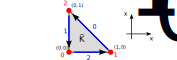
\includegraphics[width=1\linewidth]{figures/reference_triangle.pdf}
{\footnotesize reference triangle}
\end{center}
\end{frame}

%%%%%%%%%%%%%%%%%%%%%%%%%%%%%%%%%%%%%%%%%%%%%%%%%%%%%%%%%%%%%%%%%%

\begin{frame}
\frametitle{Function space}
Polynomials of degree $p$
$$
\begin{aligned}
\mathcal{V}_h &= \mathcal{P}_p(\widehat{K})\subset H^1(\widehat{K})\\
&= \Big\{q:q(x) = \sum_{\substack{s_0,s_1\\s_0+s_1\le p}} a_{s_0,s_1} x_0^{s_0}x_1^{s_1}\;\text{$\forall\;x\in \widehat{K}$ with $a_{s_0,s_1}\in\mathbb{R}$}\Big\}
\end{aligned}
$$
\textbf{Basis functions}
$$
\{\phi_\ell\}_{\ell=0}^{\nu-1}\qquad\text{with $n_{\text{dof}}=\nu = {p+2 \choose 2} = \frac{1}{2}(p+2)(p+1)$}
$$
Naive choice: monomials
$$
\{\phi_\ell\}_{\ell=0}^{\nu-1} = \{1,x_0,x_1,x_0^2,x_0x_1,x_1^2,\dots\}
$$
Better choice: \textbf{Lagrange polynomials}
\end{frame}

%%%%%%%%%%%%%%%%%%%%%%%%%%%%%%%%%%%%%%%%%%%%%%%%%%%%%%%%%%%%%%%%%%

\begin{frame}
\frametitle{Lagrange polynomials}
\textbf{One dimension}\\
Lagrange polynomial $p$ = unique polynomial of degree $m$ which passes through $m+1$ points $\{(t_k,z_k)\}_{k=0}^{m}$:
$$
p(t_k)=z_k\qquad\text{for all $k=0,1,\dots,m$}
$$
\begin{center}
\includegraphics[width=0.55\linewidth]{figures/lagrange_polynomials_1d.png}
\end{center}
\textbf{Two dimensions}\\
Choose $\nu$ points $\{\xi^{(\ell)}\}_{\ell=0}^{\nu-1}$ in $\widehat{K}$ and define $\phi_\ell(x)\in\mathcal{P}_p(K)$ such that
$$
\phi_\ell(\xi^{(k)}) = \delta_{\ell k} = \begin{cases}
    1 & \text{for $\ell=k$}\\
    0 & \text{otherwise}.
\end{cases}
$$
\end{frame}

%%%%%%%%%%%%%%%%%%%%%%%%%%%%%%%%%%%%%%%%%%%%%%%%%%%%%%%%%%%%%%%%%%

\begin{frame}
\frametitle{Lagrange polynomials}
\textbf{Nodal points}\\[-3ex]
$$
\{\xi^{(\ell)}\}_{\ell=0}^{\nu-1} = \left\{\left(\frac{\ell_0}{p},\frac{\ell_1}{p}\right) \quad \text{for $\ell_0,\ell_1\in\mathbb{N}$ with $0\le \ell_0\le \ell_1 \le p$}\right\}
$$
\begin{center}
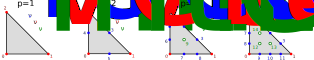
\includegraphics[width=0.9\linewidth]{figures/lagrange_nodes.pdf}
\end{center}
\textbf{Ordering of points}\\[1ex]
\begin{minipage}{0.75\linewidth}
\begin{itemize}
  \item $\nu_{\text{vertex}}=1$ point associated with each vertex \textcolor{red}{$v_0$}, \textcolor{red}{$v_1$}, \textcolor{red}{$v_2$} (in this order); 
  \item $\nu_{\text{facet}}=p-1$ points associated with each facet \textcolor{blue}{$F_0$}, \textcolor{blue}{$F_1$}, \textcolor{blue}{$F_2$} (in this order), numbered following arrows
  \item $\nu_{\text{interior}}=\frac{1}{2}(p-1)(p-2)$ points associated with interior $K^0$
\end{itemize}
\end{minipage}
\hfill
\begin{minipage}{0.225\linewidth}
  \begin{center}
  \includegraphics[width=\linewidth]{figures/reference_triangle_small.pdf}
  \end{center}
\end{minipage}
\end{frame}

%%%%%%%%%%%%%%%%%%%%%%%%%%%%%%%%%%%%%%%%%%%%%%%%%%%%%%%%%%%%%%%%%%

\begin{frame}
\frametitle{Examples}

\textbf{Linear finite element} $p=1$
$$
\begin{aligned}
\phi_0(x) &= 1-x_0-y_0\\
\phi_1(x) &= x_0\\
\phi_2(x) &= x_1
\end{aligned}
$$
$\nu_{\text{vertex}}=1$, $\nu_{\text{facet}}=\nu_{\text{interior}}=0$
\end{frame}

%%%%%%%%%%%%%%%%%%%%%%%%%%%%%%%%%%%%%%%%%%%%%%%%%%%%%%%%%%%%%%%%%%

\begin{frame}
\frametitle{Examples}
\textbf{Quadratic element} $p=2$\qquad ($\nu_{\text{interior}}=0$)\\[1ex]
\begin{minipage}{0.475\linewidth}
vertices ($\nu_{\text{vertex}}=1$)
$$
{\footnotesize
\begin{aligned}
\phi_0(x) &= (1-x_0-x_1)(1-2x_0-2x_1),\\
\phi_1(x) &= x_0(2x_0-1),\\
\phi_2(x) &= x_1(2x_1-1),
\end{aligned}
}
$$
\end{minipage}
\hfill
\begin{minipage}{0.475\linewidth}
facets ($\nu_{\text{facet}}=1$)
$$
{\footnotesize
\begin{aligned}
\phi_3(x) &= 4x_0x_1,\\
\phi_4(x) &= 4x_1(1-x_0-x_1),\\
\phi_5(x) &= 4x_0(1-x_0-x_1),
\end{aligned}}
$$
\end{minipage}
\begin{center}
\includegraphics[width=0.9\linewidth]{figures/quadratic_element.png}
\end{center}
\end{frame}

%%%%%%%%%%%%%%%%%%%%%%%%%%%%%%%%%%%%%%%%%%%%%%%%%%%%%%%%%%%%%%%%%%

\begin{frame}
\frametitle{Dual spaces}
Domain $\Omega$, space $\mathcal{V}=\mathcal{V}(\Omega)$ of real-valued functions $w:\Omega\rightarrow \mathbb{R}$\\[1ex]
\textbf{Linear functional}
$$
\lambda : \mathcal{V} \rightarrow \mathbb{R},\qquad w \mapsto \lambda(w)\in\mathbb{R}
$$
such that for all $c_1,c_2\in\mathbb{R}$, $w^{(1)}, w^{(2)} \in \mathcal{V}$
$$
\lambda(c_1 w^{(1)}+c_2 w^{(2)}) = c_1\lambda(w^{(1)})+c_2 \lambda(w^{(2)})
$$
\textbf{Dual space} $\mathcal{V}^*$ = space of all linear functionals on $\mathcal{V}$\\[2ex]
$\text{dim}(\mathcal{V})=\text{dim}(\mathcal{V}^*)$ if $\text{dim}(\mathcal{V})<\infty$
\end{frame}

%%%%%%%%%%%%%%%%%%%%%%%%%%%%%%%%%%%%%%%%%%%%%%%%%%%%%%%%%%%%%%%%%%

\begin{frame}
\frametitle{Examples}
Let $\Omega\subset \mathbb{R}^2$ and $\mathcal{V}=H^1(\Omega)$\\[2ex]
\textbf{Linear functionals} $\lambda\in\mathcal{V}^*$
\begin{itemize}
\item \textbf{point evaluation}: $\lambda(w) := w(\xi)$ for some point $\xi\in \Omega$
\item \textbf{differentiation}: $\lambda(w) := \frac{\partial w}{\partial x_0}(\xi)$ for some point $\xi\in \Omega$
\item \textbf{integration}: $\lambda(w) := \int_\Omega fw\;dx$ for some function $f \in L_2(\Omega)$
\end{itemize}
\end{frame}

%%%%%%%%%%%%%%%%%%%%%%%%%%%%%%%%%%%%%%%%%%%%%%%%%%%%%%%%%%%%%%%%%%

\begin{frame}
\frametitle{Ciarlet's definition of the finite element}
Finite element = triple $(\widehat{K},\widehat{\mathcal{V}},\mathcal{L})$
\begin{enumerate}
\item \textbf{domain} $\widehat{K}$ (= reference triangle)
\item \textbf{function space} $\widehat{\mathcal{V}}=\widehat{\mathcal{V}}(\widehat{K})$ of real-valued functions on $\widehat{K}$
\item \textbf{degrees of freedom} {\footnotesize(or \textbf{nodes})} $\mathcal{L} = \{\lambda_\ell\}_{\ell=0}^{\nu-1}$ = basis for $\widehat{\mathcal{V}}^*$
\end{enumerate}
\vspace{2ex}
$\Rightarrow$ \textbf{nodal basis} $\{\phi_\ell\}_{\ell=0}^{\nu-1}$
$$
\lambda_\ell (\phi_k) = \delta_{\ell k} \qquad\text{for all $\ell,k=0,1,\dots,\nu-1$}
$$
\end{frame}

%%%%%%%%%%%%%%%%%%%%%%%%%%%%%%%%%%%%%%%%%%%%%%%%%%%%%%%%%%%%%%%%%%

\begin{frame}
\frametitle{Examples}
\textbf{Polynomial Lagrange element}
\begin{enumerate}
\item $\widehat{K}$ the reference triangle
\item $\widehat{\mathcal{V}} = \mathcal{P}_p(\widehat{K})$ = space of bi-variate polynomials of degree $p$
\item $\mathcal{L}=\{\lambda_\ell\}_{\ell=0}^{\nu-1}$, $\lambda_\ell(w) = w(\xi^{(\ell)})$ {\footnotesize (= evaluation at nodal points $\xi^{(\ell)}$)}
\end{enumerate}
\vspace{2ex}
Alternative choice of dofs: for some point $\mathring{\xi}\in \widehat{K}$
$$
\lambda_\ell (w) = \frac{\partial^{\ell_a}w}{\partial x_0^{\ell_b} \partial x_1^{\ell_a-\ell_b}}(\mathring{\xi}) 
$$
for $0\le \ell_b \le \ell_a\le p$ and $\ell=\frac{1}{2}\ell_a(\ell_a-1) + \ell_b$
\end{frame}

%%%%%%%%%%%%%%%%%%%%%%%%%%%%%%%%%%%%%%%%%%%%%%%%%%%%%%%%%%%%%%%%%%

\begin{frame}
\frametitle{Examples}

Two-dimensional \textbf{Argyris finite element}
\begin{enumerate}
\item $\widehat{K}$ = reference triangle
\item $\widehat{\mathcal{V}} = \mathcal{P}_5(\widehat{K})$, the space of quintic bi-variate polynomials
\item 21 nodes ($\nu_{\text{vertex}}=6$, $\nu_{\text{facet}}=1$, $\nu_{\text{interior}}=0$) defined as:
\begin{itemize}
  \item $\lambda_\rho(w) = w(v_\rho)$ {\footnotesize(evaluation at each vertex $v_\rho$ $\Rightarrow$ 3 nodes)}
  \item $\lambda_{3+2\rho+a}(w) = \frac{\partial w}{\partial x_a}(v_\rho)$\\{\footnotesize(two gradient evaluations at each vertex $v_\rho$ $\Rightarrow$ 6 nodes)}
  \item $\lambda_{9+3\rho+2a+b}(w) = \frac{\partial^2 w}{\partial x_a \partial x_b}(v_\rho)$ with $0\le a\le b\le 1$\\{\footnotesize(Hessian evaluation at each vertex $v_\rho$ $\Rightarrow$ 9 nodes)}
  \item $\lambda_{18+\rho}(w) = n_\rho\cdot \nabla w(m_\rho)$\\{\footnotesize(normal derivative evaluation at the midpoints $m_\rho$ of each facet $F_\rho$ $\Rightarrow$ 3 nodes)}
\end{itemize}
\end{enumerate}
Only differs from $p=5$ polynomial element in choice of nodes
\end{frame}

%%%%%%%%%%%%%%%%%%%%%%%%%%%%%%%%%%%%%%%%%%%%%%%%%%%%%%%%%%%%%%%%%%

\begin{frame}
\frametitle{Ordering of degrees of freedom}
Node $\leftrightarrow$ topological entity of $\widehat{K}$
\begin{minipage}{0.6\linewidth}
\textbf{topological entities}
\begin{itemize}
\item \textcolor{red}{vertices $v_0$, $v_1$, $v_2$} (in this order)
\item \textcolor{blue}{facets $F_0$, $F_1$, $F_2$} (in this order)
\item interior $K^0$
\end{itemize}
\end{minipage}
\hfill
\begin{minipage}{0.3\linewidth}
  \begin{center}
  \includegraphics[width=\linewidth]{figures/reference_triangle_small.pdf}
  \end{center}
\end{minipage}\\
Recall:
\begin{itemize}
\item $\nu_{\text{vertex}}$ nodes per vertex
\item $\nu_{\text{facet}}$ nodes per facet 
\item $\nu_{\text{interior}}$ nodes in interior $K^0$
\end{itemize}
Total number of nodes (dofs)
$$
\nu = 3( \nu_{\text{vertex}}+\nu_{\text{facet}})+\nu_{\text{interior}}.
$$
\end{frame}

%%%%%%%%%%%%%%%%%%%%%%%%%%%%%%%%%%%%%%%%%%%%%%%%%%%%%%%%%%%%%%%%%%

\begin{frame}
  \frametitle{Ordering of degrees of freedom}
Arrange degrees of freedom $\{\lambda_0,\dots,\lambda_{\nu-1}\}$ in the order
$$
\underbrace{v_0 \rightarrow v_1 \rightarrow v_2}_{\text{(vertices)}}
\rightarrow \underbrace{F_0 \rightarrow F_1 \rightarrow F_2}_{\text{(facets)}}
\rightarrow \underbrace{K^0}_{\text{(interior)}}
$$
$\lambda_j^{(E_\rho)}$ = $j$-th node associated with $E_\rho\in \{v_0,v_1,v_2,F_0,F_1,F_2,K^0\}$
\begin{center}
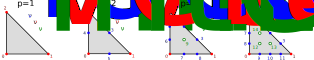
\includegraphics[width=0.8\linewidth]{figures/lagrange_nodes.pdf}
\end{center}
$$
\begin{aligned}
& \{\lambda_0^{(v_0)},\dots,\lambda_{\nu_{\text{vertex}}-1}^{(v_0)},
\lambda_0^{(v_1)},\dots,\lambda_{\nu_{\text{vertex}}-1}^{(v_1)},
\lambda_0^{(v_2)},\dots,\lambda_{\nu_{\text{vertex}}-1}^{(v_2)},\\
& \lambda_0^{(F_0)},\dots,\lambda_{\nu_{\text{facet}}-1}^{(F_0)},
\lambda_0^{(F_1)},\dots,\lambda_{\nu_{\text{facet}}-1}^{(F_1)},
\lambda_0^{(F_2)},\dots,\lambda_{\nu_{\text{facet}}-1}^{(F_2)},\\
& \lambda_0^{(K^0)},\dots,\lambda_{\nu_{\text{interior}}-1}^{(K^0)}
\}
\end{aligned}
$$
\end{frame}

%%%%%%%%%%%%%%%%%%%%%%%%%%%%%%%%%%%%%%%%%%%%%%%%%%%%%%%%%%%%%%%%%%

\begin{frame}
\frametitle{Ordering of degrees of freedom}
\textbf{Indirection map} $\mu_{\text{dof}}$: $\lambda_{\ell=\mu_{\text{dof}}(E,\rho,j)} = \lambda_j^{(E_\rho)}$
$$
\mu_{\text{dof}}(E,\rho,j) = \begin{cases}
\rho\cdot \nu_{\text{vertex}} + j & \text{if $E_\rho$ is the $\rho$-th vertex}\\
3\nu_{\text{vertex}} + \rho\cdot \nu_{\text{facet}} + j & \text{if $E_\rho$ is the $\rho$-th facet}\\
3(\nu_{\text{vertex}} + \nu_{\text{facet}}) + j & \text{if $E$ is the interior}
\end{cases}
$$
Example: \textbf{quartic Lagrange element} ($p=4$)\\[2ex]
\begin{minipage}{0.3\linewidth}
$$
\begin{aligned}
\mu_{\text{dof}}(v,1,0) &= 1\\
\mu_{\text{dof}}(F,0,2) &= 5\\
\mu_{\text{dof}}(K^0,0,2) &= 14
\end{aligned}
$$
\end{minipage}
\hfill
\begin{minipage}{0.3\linewidth}
  \begin{center}
  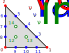
\includegraphics[width=\linewidth]{figures/lagrange_nodes_quintic.pdf}
  \end{center}
\end{minipage}
\hfill
\begin{minipage}{0.3\linewidth}
  \begin{center}
  \includegraphics[width=\linewidth]{figures/reference_triangle_small.pdf}
  \end{center}
\end{minipage}
\end{frame}

%%%%%%%%%%%%%%%%%%%%%%%%%%%%%%%%%%%%%%%%%%%%%%%%%%%%%%%%%%%%%%%%%%

\begin{frame}
\frametitle{Vandermonde matrix}
\textbf{Nodal basis functions} $\{\phi_\ell(x)\}_{\ell=0}^{\nu-1}$\\
Start with basis of $\widehat{\mathcal{V}}$:
$$
\{\theta_m(x)\}_{m=0}^{\nu-1}=\{1,x_0,x_1,x_0^2,x_0x_1,x_1^2,\dots\}
$$
and expand
$$
\phi_k(x) = \sum_{m=0}^{\nu-1} c_m^{(k)} \theta_m(x)\qquad\text{for coefficients $c_m^{(k)}$}
$$
Definition of nodal basis
$$
\delta_{\ell k} = \lambda_\ell(\phi_k) = \sum_{m=0}^{\nu-1} \underbrace{c_m^{(k)}}_{C_{mk}} \underbrace{\lambda_\ell(\theta_m)}_{V_{\ell m}}
$$
\end{frame}

%%%%%%%%%%%%%%%%%%%%%%%%%%%%%%%%%%%%%%%%%%%%%%%%%%%%%%%%%%%%%%%%%%

\begin{frame}
\frametitle{Vandermonde matrix}

Define $\nu\times\nu$ matrices $V$, $C$ with $V_{\ell m} := \lambda_\ell(\theta_m)$ and $C_{mk}:=c_m^{(k)}$

$$
\delta_{\ell k} =  \sum_{m=0}^{\nu-1} c_m^{(k)} \lambda_\ell(\theta_m)
\quad \Leftrightarrow \quad
VC = \mathbb{I}\quad \Leftrightarrow \quad C = V^{-1}
$$
Lagrange element $\lambda_\ell(w) = w(\xi^{(\ell)})$ $\Rightarrow$ $V_{\ell m} = \lambda_{\ell}(\theta_m) = \theta_m(\xi^{(\ell)})$\\[1ex]
\textbf{Vandermonde matrix}
$$
\setlength\arraycolsep{2pt}
{\footnotesize%
V = V(\{\xi^{(\ell)}\}_{\ell=0}^{\nu-1}) = \begin{pmatrix}
1 & \xi^{(0)}_0 & \xi^{(0)}_1  & (\xi^{(0)}_0)^2 & \xi^{(0)}_0 \xi^{(0)}_1 & (\xi^{(0)}_1)^2 & \dots \\[1ex]
1 & \xi^{(1)}_0 & \xi^{(1)}_1 & (\xi^{(1)}_0)^2 & \xi^{(1)}_0 \xi^{(1)}_1 & (\xi^{(1)}_1)^2 & \dots \\[1ex]
1 & \xi^{(2)}_0 & \xi^{(2)}_1 & (\xi^{(2)}_0)^2 & \xi^{(2)}_0 \xi^{(2)}_1 & (\xi^{(2)}_1)^2 & \dots \\[1ex]
\vdots & \vdots & \vdots & \vdots & \vdots & \vdots & \ddots\\
1 & \xi^{(\nu-1)}_0 & \xi^{(\nu-1)}_1 & (\xi^{(\nu-1)}_0)^2 & \xi^{(\nu-1)}_0 \xi^{(\nu-1)}_1 & (\xi^{(\nu-1)}_1)^2 & \dots
\end{pmatrix}}
$$
\textbf{Nodal basis functions}
$$
\phi_k(x) = \sum_{m=0}^{\nu-1} C_{mk} \theta_m(x)\qquad\text{with $C_{mk} = (V^{-1})_{mk}$}
$$
\end{frame}

%%%%%%%%%%%%%%%%%%%%%%%%%%%%%%%%%%%%%%%%%%%%%%%%%%%%%%%%%%%%%%%%%%

\begin{frame}
\frametitle{Evaluation of basis functions}
Consider any $n$ points
$$
\boldsymbol{\zeta}:=\{\zeta^{(r)}\}_{r=0}^{n-1}\qquad\text{with $\zeta^{(r)}\in\widehat{K}$}
$$
Define
\begin{itemize}
\item $n\times\nu$ matrix $V(\boldsymbol{\zeta})$
$$
V_{rm}(\boldsymbol{\zeta}) := \theta_m(\zeta^{(r)})
$$
\item Rank 3 tensor $V^{\partial}(\boldsymbol{\zeta})$ of shape $[n,\nu,2]$
$$
V^{\partial}_{rma}(\boldsymbol{\zeta}):=\frac{\partial \theta_m}{\partial x_a}(\zeta^{(r)}).
$$
\end{itemize}
\end{frame}

%%%%%%%%%%%%%%%%%%%%%%%%%%%%%%%%%%%%%%%%%%%%%%%%%%%%%%%%%%%%%%%%%%

\begin{frame}
\frametitle{Tabulation of basis functions}
\textbf{Evaluation of nodal basis functions}: $n\times \nu$ matrix $T(\vec{\zeta})$
$$
T_{r\ell}(\boldsymbol{\zeta}) := \phi_\ell(\zeta^{(r)}) = \sum_{m=0}^{\nu-1} c_m^{(\ell)} \theta_m(\zeta^{(r)}) = \sum_{m=0}^{\nu-1}V_{rm}(\boldsymbol{\zeta})C_{m\ell}
$$
$$
T(\boldsymbol{\zeta}) = V(\boldsymbol{\zeta}) C\qquad\text{with $C=V^{-1}$}
$$
\textbf{Evaluation of derivatives}: rank 3 tensor $T^\partial(\vec{\zeta})$ of shape $[n,\nu,2]$
$$
\begin{aligned}
T^\partial_{r\ell a}(\boldsymbol{\zeta}) &:= \frac{\partial \phi_\ell}{\partial x_a}(\zeta^{(r)}) 
 = \sum_{m=0}^{\nu-1} c_m^{(\ell)} \frac{\partial \theta_m}{\partial x_a}(\zeta^{(r)}) \\
 &= \sum_{m=0}^{\nu-1} V^\partial_{rma}(\boldsymbol{\zeta})C_{m\ell}
 \end{aligned}
$$
\end{frame}


%%%%%%%%%%%%%%%%%%%%%%%%%%%%%%%%%%%%%%%%%%%%%%%%%%%%%%%%%%%%%%%%%%

\begin{frame}
\frametitle{Implementation}
Ciarlet's definition of finite element\\[1ex]
$\Rightarrow$
\textbf{Abstract base class} \lstinline{FiniteElement}
\begin{itemize}
\item \# nodes associated with each topological entity
\begin{itemize}
  \item abstract properties \lstinline{ndof_per_vertex}, \lstinline{ndof_per_facet}, \lstinline{ndof_per_interior} for $\nu_{\text{vertex}}$, $\nu_{\text{facet}}$ and $\nu_{\text{interior}}$. 
  \item property \lstinline{ndof}: $\nu =3(\nu_{\text{vertex}}+\nu_{\text{facet}})+\nu_{\text{interior}}$
\end{itemize}
\item Tabulate evaluation of dofs for given $\hat{f}$ $\Rightarrow$ abstract method \lstinline{tabulate_dofs(fhat)} returns $(\lambda_0(\hat{f}),\lambda_1(\hat{f}),\dots,\lambda_{\nu-1}(\hat{f}))^\top$
\item Tabulate basis functions for $\boldsymbol{\zeta}=\{\zeta^{(r)}\}_{r=0}^{n-1}$ $\Rightarrow$ abstract method \lstinline{tabulate(zeta)} returns $n\times\nu$ matrix $T$ with $T_{r\ell}=\phi_\ell(\zeta^{(r)})$ 
\item Tabulate gradients of basis functions for $\boldsymbol{\zeta}=\{\zeta^{(r)}\}_{r=0}^{n-1}$ $\Rightarrow$ abstract method \lstinline{tabulate_gradient(zeta)} returns rank 3 tensor $T^\partial$ of shape $n\times\nu\times 2$ with $T^\partial_{r\ell a}=\frac{\partial\phi_\ell}{\partial x_a}(\zeta^{(r)})$. 
\item dof-map $\mu_{\text{dof}}(E,\rho,j)$ and its inverse\\$\Rightarrow$ \lstinline{dofmap(entity_type,rho,j)}, \lstinline{inverse_dofmap(ell)}
\end{itemize}
\end{frame}

%%%%%%%%%%%%%%%%%%%%%%%%%%%%%%%%%%%%%%%%%%%%%%%%%%%%%%%%%%%%%%%%%%

\begin{frame}
\frametitle{Concrete implementations}
\textbf{Subclassing} the \lstinline{FiniteElement} base class\\
$\Rightarrow$ Provide concrete implementations of:
\begin{itemize}
\item \# dofs associated with topological entities:\\\lstinline{ndof_per_vertex}, \lstinline{ndof_per_facet} and \lstinline{ndof_per_interior}
\item Evalute dofs for given function $\widehat{f}$: \lstinline{tabulate_dofs(fhat)} 
\item Tabulate basis functions: \lstinline{tabulate(zeta)}
\item Tabulate gradients of basis functions: \lstinline{tabulate_gradient(zeta)}
\end{itemize}
\end{frame}

%%%%%%%%%%%%%%%%%%%%%%%%%%%%%%%%%%%%%%%%%%%%%%%%%%%%%%%%%%%%%%%%%%

\begin{frame}[fragile]
\frametitle{Concrete implementations}
Available finite elements
\begin{itemize}
\item Bi-linear element $(p=1)$: \lstinline{LinearElement}
\item Cubic linear element $(p=3)$: \lstinline{CubicElement} (= exercise)
\item General polynomial element: \lstinline{PolynomialElement} (will be made available later)
\end{itemize}
\vspace{2ex}
Import as
\begin{lstlisting}
from fem.linearelement import LinearElement
from fem.polynomialelement import PolynomialElement
\end{lstlisting}
\end{frame}

%%%%%%%%%%%%%%%%%%%%%%%%%%%%%%%%%%%%%%%%%%%%%%%%%%%%%%%%%%%%%%%%%%

\begin{frame}
\frametitle{Numerical quadrature}
The weak form of PDE requires \textbf{integration} over domain $\Omega$
$$
a(u,v) = \int_\Omega \left(\kappa \nabla u \cdot \nabla  v + \omega\; u v\right)\;dx
$$
\textbf{Numerical integration in 1d}
$$
\int_{-1}^{+1} f(z)\;dz \approx \sum_{q=0}^{n_q-1} \widetilde{w}_q f(\widetilde{\zeta}^{(q)})
$$
\textbf{Qudrature\footnote{often called ``cubature'' in more than one dimension} rule} $\mathcal{Q}=\{(\widetilde{\zeta}^{(q)},\widetilde{w}_q)\}_{q=0}^{n_q-1}$
\begin{itemize}
\item points $\widetilde{\zeta}^{(q)}$, $q=0,1,2,\dots,n_q-1$
\item corresponding weights $\widetilde{w}_q$
\end{itemize}
\end{frame}

%%%%%%%%%%%%%%%%%%%%%%%%%%%%%%%%%%%%%%%%%%%%%%%%%%%%%%%%%%%%%%%%%%

\begin{frame}[fragile]
\frametitle{Numerical quadrature}
\textbf{Gauss-Legendre quadrature} $\mathcal{Q}^{(\text{GL})}_{n_q}$
\begin{itemize}
 \item points $\widetilde{\zeta}^{(q)}$ = roots of the Legendre polynomial $P_{n_q}$
 \item weights $\widetilde{w}_q = \frac{2}{(1-(\widetilde{\zeta}^{(q)})^2)(P_{n_q}'(\widetilde{\zeta}^{(q)}))^2}$
\end{itemize}

\begin{lstlisting}
points, weights = numpy.polynomial.legendre.leggauss(n_q)
\end{lstlisting}
\textbf{Exact} for polynomials of degree $2n_q-1$:

$$
\int_{-1}^{+1} p(z)\;dz = \sum_{q=0}^{n_q-1} \widetilde{w}_q p(\widetilde{\zeta}^{(q)})\qquad\text{for $p\in\mathcal{P}_{2n_q-1}$}
$$
\textbf{degree of precision} (dop)
$$
\text{dop}(\mathcal{Q}^{(\text{GL})}_{n_q}) = 2n_q-1
$$
\end{frame}

%%%%%%%%%%%%%%%%%%%%%%%%%%%%%%%%%%%%%%%%%%%%%%%%%%%%%%%%%%%%%%%%%%

\begin{frame}[fragile]
\frametitle{Numerical quadrature}
\textbf{Lowest order Gauss-Legendre} quadrature rules
\begin{center}
  \renewcommand{\arraystretch}{2.5}
  \begin{tabular}{cccc}
    \hline
    \# points $n_q$ & points $\widetilde{\zeta}^{(q)}$ & weights $\widetilde{w}_q$ & $\text{dop}(\mathcal{Q}^{(\text{GL})}_{n_q})$\\
    \hline\hline
 1   & $0$ & $2$ & $1$\\
 2   & $-\sqrt{\frac{1}{3}}, +\sqrt{\frac{1}{3}}$ & $1$ & $3$\\
 3   & $-\sqrt{\frac{3}{5}},0,+\sqrt{\frac{3}{5}}$ & $\frac{5}{9},\frac{8}{9},\frac{5}{9}$ & $5$\\
 \hline
  \end{tabular}
\end{center}
\end{frame}

%%%%%%%%%%%%%%%%%%%%%%%%%%%%%%%%%%%%%%%%%%%%%%%%%%%%%%%%%%%%%%%%%%

\begin{frame}[fragile]
\frametitle{Integration along a line}
\textbf{Integrate function along a straight line} $\mathcal{C}\subset \mathbb{R}^2$ connecting two points $a,b\in \mathbb{R}^2$\\[1ex]
\begin{minipage}{0.6\linewidth}
Parametrisation $\gamma: [-1,1] \rightarrow \mathbb{R}^2$ 
\end{minipage}
\hfill
\begin{minipage}{0.25\linewidth}
  \begin{center}
  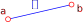
\includegraphics[width=\linewidth]{figures/straight_line.pdf}
  \end{center}
\end{minipage}
$$
\gamma(z) = \frac{1-z}{2}a+\frac{1+z}{2}b\qquad\text{\footnotesize note: $\gamma(-1)=a$, $\gamma(1)=b$}
$$
$$
\begin{aligned}
\Rightarrow\quad \int_{\mathcal{C}} f(x)\;ds &= \frac{\|b-a\|}{2} \int_{-1}^{+1} f(\gamma(z))\;dz \approx \sum_{q=0}^{n_q-1} w_{\mathcal{C},q} f(\zeta_{\mathcal{C}}^{(q)})
\end{aligned}
$$

\textbf{GL quadrature rule on $\mathcal{C}$}: $\mathcal{Q}^{(\text{GL},\mathcal{C})}_{n_q}=\{(\zeta^{(q)}_{\mathcal{C}},w_{\mathcal{C},q})\}_{q=0}^{n_q-1}$
$$
\zeta_{\mathcal{C}}^{(q)} = \gamma(\widetilde{\zeta}^{(q)}) = \frac{1}{2}(1-\widetilde{\zeta}^{(q)})a + \frac{1}{2}(1+\widetilde{\zeta}^{(q)})b,\qquad
w_{\mathcal{C},q} = \frac{\|b-a\|}{2} \widetilde{w}_q
$$
$$
\text{dop}(\mathcal{Q}^{(\text{GL},\mathcal{C})}_{n_q}) = \text{dop}(\mathcal{Q}^{(\text{GL})}_{n_q}) = 2n_q-1.
$$
\end{frame}

%%%%%%%%%%%%%%%%%%%%%%%%%%%%%%%%%%%%%%%%%%%%%%%%%%%%%%%%%%%%%%%%%%

\begin{frame}[fragile]
\frametitle{Two-dimensional quadrature for the reference triangle}
Duffy transform $\tau$: $S=[-1,+1]\times [-1,+1]\mapsto \widehat{K} = \tau(S)$
$$
\begin{aligned}
\tau(\widetilde{x}) = \begin{pmatrix}\frac{1}{2}(1+\widetilde{x}_0)\\[1ex]\frac{1}{4}(1-\widetilde{x}_0)(1+\widetilde{x}_1)\end{pmatrix} \in \widehat{K}\qquad\text{for $\widetilde{x}=(\widetilde{x}_0,\widetilde{x}_1)\in S$}
\end{aligned}
$$
\begin{center}
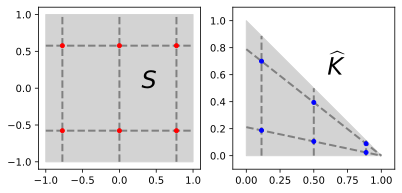
\includegraphics[width=0.5\linewidth]{figures/quadrature.pdf}
\end{center}
\textbf{Quadrature on} $\boldsymbol{S}=[-1,+1]\times[-1,+1]$ $\Rightarrow$ product of 1d rules\\$\mathcal{Q}_{n_q+1}^{(\text{GL})} = \{(\widetilde{\zeta}^{(q_0)}_0,\widetilde{w}_{0,q_1})\}_{q_0=0}^{n_q}$, $\mathcal{Q}_{n_q}^{(\text{GL})} =\{(\widetilde{\zeta}^{(q_1)}_1,\widetilde{w}_{1,q_1})\}_{q_1=0}^{n_q-1}$\\[1ex]
2d quadrature rule $\mathcal{Q}_{n_q}^{(\text{GL},S)}=\{(\widetilde{\zeta}^{(q)},\widetilde{w}_q)\}_{q=0}^{N_q-1}$, $N_q = n_q(n_q+1)$
$$
\widetilde{\zeta}^{(q)} = \begin{pmatrix}\widetilde{\zeta}^{(q_0)}_0\\[1ex]\widetilde{\zeta}^{(q_1)}_1\end{pmatrix}\in\mathbb{R}^2,\quad \widetilde{w}_i = \widetilde{w}_{0,q_0}\cdot \widetilde{w}_{1,q_1} \qquad \text{$q=n_q q_0+q_1$}.
$$
\end{frame}

%%%%%%%%%%%%%%%%%%%%%%%%%%%%%%%%%%%%%%%%%%%%%%%%%%%%%%%%%%%%%%%%%%

\begin{frame}[fragile]
\frametitle{Two-dimensional quadrature for the reference triangle}
\textbf{Integration over $\boldsymbol{\widehat{K}}$}\\
Duffy transform $\tau$ $\Rightarrow$ quadrature rule on $\widehat{K}$ $\mathcal{Q}_{n_q}^{(\text{GL},\widehat{K})} = \{(\zeta^{(q)},w_q)\}_{q=0}^{N_q-1} = \tau(\mathcal{Q}^{(S)}_{n_q})$ over $\widehat{K}$:

$$
\begin{aligned}
\zeta^{(q)} &= \tau(\widetilde{\zeta}^{(q)}) = \begin{pmatrix}(\frac{1}{2}(1+\widetilde{\zeta}^{(q_0)}_0)\\[1ex]\frac{1}{4}(1-\widetilde{\zeta}^{(q_0)}_0)(1+\widetilde{\zeta}^{(q_1)}_1)\end{pmatrix}\qquad \text{where $q=n_qq_0+q_1$}\\
w_q &= \widetilde{w}_q \left|\det\left(\frac{\partial \tau}{\partial \widetilde{x}}\right)\right|_{\widetilde{x}=\widetilde{\zeta}^{(q)}}= \frac{1}{8}\widetilde{w}_{0,q_0}\widetilde{w}_{1,q_1}(1-\widetilde{\zeta}^{(q_0)}_0)
\end{aligned}
$$
\begin{center}
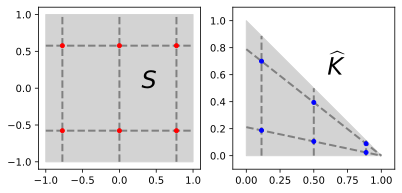
\includegraphics[width=0.5\linewidth]{figures/quadrature.pdf}
\end{center}
$$
\text{dop}(\mathcal{Q}^{(\text{GL},\widehat{K})}_{n_q}) = \text{dop}(\mathcal{Q}^{(\text{GL})}_{n_q}) = 2n_q-1.
$$
\end{frame}

%%%%%%%%%%%%%%%%%%%%%%%%%%%%%%%%%%%%%%%%%%%%%%%%%%%%%%%%%%%%%%%%%%

\begin{frame}[fragile]
\frametitle{Implementation in Python}
\textbf{Abstract base class} \lstinline{Quadrature}
\begin{itemize}
\item Points $\{\zeta^{(q)}\}_{q=0}^{n_q-1}$ $\Rightarrow$ array \lstinline{nodes} of shape $n_q\times 2$
\item Weights $\{w_q\}_{q=0}^{n_q-1}$ $\Rightarrow$ array \lstinline{weights} of length $n_q$
\item degree of precision $\Rightarrow$ property \lstinline{degree_of_precision}
\end{itemize}
\vspace{2ex}
Concrete implementations in \textbf{subclasses}
\begin{itemize}
  \item Quadrature rule $\mathcal{Q}^{(\text{GL},\mathcal{C})}_{n_q}$ over line segment $\mathcal{C}$: \lstinline{GaussLegendreQuadratureLineSegment(v_a, v_b, npoints)}
  \begin{itemize}
    \item \lstinline{v_a} start point $a$
    \item \lstinline{v_b} end point $b$
    \item \lstinline{npoints} number of points $n_q$
  \end{itemize}
  \item Quadrature rule $\mathcal{Q}^{(\text{GL},\widehat{K})}_{n_q}$ over the reference triangle $\widehat{K}$: \lstinline{GaussLegendreQuadratureReferenceTriangle(npoints)}
\end{itemize}
\end{frame}

%%%%%%%%%%%%%%%%%%%%%%%%%%%%%%%%%%%%%%%%%%%%%%%%%%%%%%%%%%%%%%%%%%

\section{Local assembly}

%%%%%%%%%%%%%%%%%%%%%%%%%%%%%%%%%%%%%%%%%%%%%%%%%%%%%%%%%%%%%%%%%%

\begin{frame}
  \tableofcontents[currentsection]
\end{frame}

%%%%%%%%%%%%%%%%%%%%%%%%%%%%%%%%%%%%%%%%%%%%%%%%%%%%%%%%%%%%%%%%%%

\begin{frame}
\frametitle{Finite element method on triangle}
Putting it all together\\[2ex]
\textbf{Solve}
$$
\begin{aligned}
-\nabla\cdot(\kappa \cdot u) + \omega u &= f\qquad\text{in $\Omega=\widehat{K}$}\\
\kappa\; n\cdot \nabla u&=g \qquad\text{on $\partial\Omega$}
\end{aligned}
$$
\begin{itemize}
\item assemble stiffness matrix $A^{(h)}$
$$
A^{(h)}_{\ell k} = a(\phi_k,\phi_\ell) = \int_{\widehat{K}} \Big(\kappa \nabla \phi_k(x) \cdot\nabla\phi_\ell(x) + \omega\; \phi_k(x) \phi_\ell(x)\Big)\;dx
$$
\item assemble right-hand side vector $\boldsymbol{b}^{(h)}$
$$
b^{(h)}_\ell = b(\phi_\ell) = \int_{\widehat{K}} f(x)\phi_\ell(x)\;dx + \int_{\partial \widehat{K}} g(x)\phi_\ell(x)\;dx
$$
\end{itemize}
\end{frame}

%%%%%%%%%%%%%%%%%%%%%%%%%%%%%%%%%%%%%%%%%%%%%%%%%%%%%%%%%%%%%%%%%%

\begin{frame}
\frametitle{Stiffness matrix}
\textbf{Entries of stiffness matrix $\boldsymbol{A^{(h)}}$} (in $d=2$ dimensions)
$$
\begin{aligned}
A^{(h)}_{\ell k}  &= \int_{\widehat{K}} \Big(\kappa \nabla \phi_k(x) \cdot\nabla\phi_\ell(x) + \omega\; \phi_k(x) \phi_\ell(x)\Big)\;dx\\
&= \int_{\widehat{K}} \left(\kappa \sum_{a=0}^{d-1}\frac{\partial\phi_k}{\partial x_a}(x) \frac{\partial\phi_\ell}{\partial x_a}(x) + \omega\; \phi_k(x) \phi_\ell(x)\right)\;dx\\
&\approx 
\sum_{q=0}^{N_q-1} w_q\left(\kappa \sum_{a=0}^{d-1}\frac{\partial\phi_k}{\partial x_a}(\zeta^{(q)}) \frac{\partial\phi_\ell}{\partial x_a}(\zeta^{(q)}) + \omega\; \phi_k(\zeta^{(q)}) \phi_\ell(\zeta^{(q)})\right)\\
&= \kappa \sum_{q=0}^{N_q-1}\sum_{a=0}^{d-1} w_q  T^\partial_{qk a} (\boldsymbol{\zeta})T^\partial_{q\ell a} (\boldsymbol{\zeta})
+\omega \sum_{q=0}^{N_q-1} w_qT_{qk}(\boldsymbol{\zeta})T_{q\ell}(\boldsymbol{\zeta})
\end{aligned}
$$
\begin{itemize}
  \item Lagrange element of degree $p$, basis functions $\{\phi_\ell\}_{\ell=0}^{\nu-1}$
  \item Quadrature $\mathcal{Q}_{p+1}^{(\text{GL},\widehat{K})}=\{w_q,\zeta^{(q)}\}_{q=0}^{N_q-1}$ with $\text{dop}=2p+1$
  \item Tabulation matrices $T$, $T^\partial$ of $\phi$, $\nabla\phi$
\end{itemize}
\end{frame}

%%%%%%%%%%%%%%%%%%%%%%%%%%%%%%%%%%%%%%%%%%%%%%%%%%%%%%%%%%%%%%%%%%

\begin{frame}
\frametitle{Right-hand side vector}
\textbf{Entries of right-hand side vector $\boldsymbol{b^{(h)}}$}
$$
\begin{aligned}
b^{(h)}_\ell  &= \int_{\widehat{K}} f(x)\phi_\ell(x)\;dx + \int_{\partial \widehat{K}} g(x)\phi_\ell(x)\;dx\\
&\approx \sum_{q=0}^{N_q-1} w_q f(\zeta^{(q)}) \phi_\ell(\zeta^{(q)}) + \sum_{\text{facets}\;F_\rho} \sum_{q=0}^{n_q-1 }w_{F_\rho,q} g(\zeta_{F_\rho}^{(q)})\phi_\ell(\zeta_{F_\rho}^{(q)}) \\
&= \sum_{q=0}^{N_q-1} w_q f_q(\boldsymbol{\zeta}) T_{q\ell}(\boldsymbol{\zeta}) + \sum_{\text{facets}\;F_\rho} \sum_{q=0}^{n_q-1 }w_{F_\rho,q} g_{q}(\boldsymbol{\zeta}_{F_\rho})T_{q\ell}(\boldsymbol{\zeta}_{F_\rho})
\end{aligned}
$$
\begin{itemize}
  \item Function evaluation at quadrature points:\\$f_q(\boldsymbol{\zeta}):=f(\zeta^{(q)})$, $g_{q}(\boldsymbol{\zeta}_{F_\rho}) := g(\zeta_{F_\rho}^{(q)})$
  \item Quadrature rule on facet $F_\rho$: $\mathcal{Q}_{p+1}^{(\text{GL},F_\rho)} = \{w_{F_\rho,q},\zeta^{(q)}_{F_\rho}\}_{q=0}^{p}$
\end{itemize}
\end{frame}

%%%%%%%%%%%%%%%%%%%%%%%%%%%%%%%%%%%%%%%%%%%%%%%%%%%%%%%%%%%%%%%%%%

\begin{frame}
\frametitle{Error}
 \textbf{Difference between exact and numerical solution}
$$
e_h(x) = u(x)-u_h(x) = u(x) - \sum_{\ell=0}^{\nu-1} u^{(h)}_\ell \phi_\ell(x)\qquad\text{for all $x\in\widehat{K}$}
$$
Square of the \textbf{$\boldsymbol{L_2}$ error norm}
$$
\begin{aligned}
\|e_h\|_{L_2(\widehat{K})}^2 &= \int_{\widehat{K}} \Big(u(x) - \sum_{j=0}^{\nu-1} u^{(h)}_\ell \phi_\ell(x)\Big)^2\;dx\\
&\approx 
\sum_{q=0} ^{N_q-1} w_q \Big(u(\zeta^{(q)}) - \sum_{\ell=0}^{\nu-1} u^{(h)}_\ell \phi_\ell(\zeta^{(q)})\Big)^2 = \sum_{q=0} ^{N_q-1} w_q e_q^2
\end{aligned}
$$
\begin{itemize}
\item Quadrature rule $\mathcal{Q}_{n_q}^{(\widehat{K})}=\{w_q,\zeta^{(q)}\}_{q=0}^{N_q-1}$
\item Error at quadrature points $e_q = u(\zeta^{(q)}) - \sum_{\ell=0}^{\nu-1} u^{(h)}_\ell T_{q\ell}$
\end{itemize}
\end{frame}

%%%%%%%%%%%%%%%%%%%%%%%%%%%%%%%%%%%%%%%%%%%%%%%%%%%%%%%%%%%%%%%%%%

\begin{frame}
\frametitle{Numerical experiment}
\textbf{Method of manufactured solutions}\\
Assume that exact solution is
$$
u(x) = u_{\text{exact}}(x) = \exp\left[-\frac{1}{2\sigma^2}(x-x_0)^2\right]
$$
$\Rightarrow$ pick $f$, $g$ to satisfy  $-\nabla\cdot(\kappa \cdot u) + \omega u = f$, $\kappa\; n\cdot \nabla u=g$

$$
\begin{aligned}
f(x) &= \left(\left(2\frac{\kappa}{\sigma^2}+\omega\right)-\frac{\kappa}{\sigma^4}(x-x_0)^2\right) u_{\text{exact}}(x)
\\
g(x) &= -\frac{\kappa}{\sigma^2}n\cdot(x-x_0)u_{\text{exact}}(x)
\end{aligned}
$$
\begin{minipage}{0.7\linewidth}
\textbf{Solution procedure}
\begin{itemize}
\item Assemble $A^{(h)}$ and $\boldsymbol{b}^{(h)}$
\item Solve linear system $A^{(h)}\boldsymbol{u}^{(h)}=\boldsymbol{b}^{(h)}$
\item Compute $L_2$ error norm $\|e_h\|_{L_2(\widehat{K})}$
\end{itemize}
\end{minipage}
\hfill
\begin{minipage}{0.25\linewidth}
  \begin{center}
    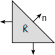
\includegraphics[width=\linewidth]{figures/reference_triangle_normals.pdf}
  \end{center}
\end{minipage}\\
\end{frame}

%%%%%%%%%%%%%%%%%%%%%%%%%%%%%%%%%%%%%%%%%%%%%%%%%%%%%%%%%%%%%%%%%%

\begin{frame}
\frametitle{Numerical experiment {\footnotesize$\kappa = 0.9$, $\omega = 0.4$, $\sigma = 0.5$, $x_0 = (0.6, 0.25)$}}
\begin{center}
  \begin{minipage}{0.8\linewidth}
    \includegraphics[width=\linewidth]{figures/triangle_solution_01.png}
  \end{minipage}
  \hfill
  \begin{minipage}{0.15\linewidth}
  $p=1$
  \end{minipage}\\
  \begin{minipage}{0.8\linewidth}
    \includegraphics[width=\linewidth]{figures/triangle_solution_03.png}
  \end{minipage}
  \hfill
  \begin{minipage}{0.15\linewidth}
  $p=3$
  \end{minipage}
\end{center}
\end{frame}

%%%%%%%%%%%%%%%%%%%%%%%%%%%%%%%%%%%%%%%%%%%%%%%%%%%%%%%%%%%%%%%%%%

\section{Error analysis}

%%%%%%%%%%%%%%%%%%%%%%%%%%%%%%%%%%%%%%%%%%%%%%%%%%%%%%%%%%%%%%%%%%

\begin{frame}
  \tableofcontents[currentsection]
\end{frame}

%%%%%%%%%%%%%%%%%%%%%%%%%%%%%%%%%%%%%%%%%%%%%%%%%%%%%%%%%%%%%%%%%%

\begin{frame}
\frametitle{Error analysis}

\textbf{Sources of error}

\begin{itemize}
\item \textcolor{blue}{Modelling error:} equations provide approximate description of physical phenomenon
\item \textcolor{blue}{Discretisation error:} for finite elements
  $$\|e_h\|_{L_2(\Omega)} \le Ch^\mu$$
  \begin{itemize}
    \item increase degree $p$
    \item decrease grid spacing $h$
  \end{itemize}
\item \textcolor{blue}{Rounding error:} approximate arithmetic on $\mathbb{R}$
\end{itemize}
\end{frame}

%%%%%%%%%%%%%%%%%%%%%%%%%%%%%%%%%%%%%%%%%%%%%%%%%%%%%%%%%%%%%%%%%%

\begin{frame}
\frametitle{Error analysis}
\textbf{Results from numerical experiment}\\
{\footnotesize$\kappa = 0.9$, $\omega = 0.4$, $\sigma = 0.5$, $x_0 = (0.6, 0.25)$}
\begin{center}
\includegraphics[width=0.8\linewidth]{figures/error_reference_triangle.png}
\end{center}
\end{frame}

%%%%%%%%%%%%%%%%%%%%%%%%%%%%%%%%%%%%%%%%%%%%%%%%%%%%%%%%%%%%%%%%%%

\begin{frame}
\frametitle{Floating point numbers}
Representation of real numbers on a computer\\
\textbf{Floating point number system}
\begin{itemize}
\item base $1<\beta\in\mathbb{N}$
\item precision $0<p\in\mathbb{N}$
\item range of exponents defined by $L,U\in\mathbb{Z}$ with $L<0\le U$
\end{itemize}
$\mathbb{F}$ = all numbers $x$ of form
$$
x = \pm \underbrace{\left(d_0 + d_1\beta^{-1} + d_2\beta^{-1} + \dots+d_{p-1}\beta^{1-p}\right)}_{\text{mantissa}}\cdot\beta^E
$$
with $d_i\in \{0,1,2,\dots,\beta-1\}$, exponent $E$ with $L\le E\le U$\\[1ex]

$\mathbb{F}$ normalised $\Leftrightarrow$ $d_0>0$ $\Rightarrow$ numbers in $\mathbb{F}$ unique.

\end{frame}

%%%%%%%%%%%%%%%%%%%%%%%%%%%%%%%%%%%%%%%%%%%%%%%%%%%%%%%%%%%%%%%%%%

\begin{frame}
\frametitle{Floating point numbers}
\textbf{Example}
$$
234.7 = \left(2+3\cdot 10^{-1}+4\cdot 10^{-2} +7\cdot 10^{-3}\right)\cdot 10^2
$$
in precision 4, base 10 arithmetic\\[2ex]
Approximation
$$
234.7 \approx \left(2+3\cdot 10^{-1}+5\cdot 10^{-2}\right)\cdot 10^2 = 235
$$
in precision 3, base 10 arithmetic

\end{frame}

%%%%%%%%%%%%%%%%%%%%%%%%%%%%%%%%%%%%%%%%%%%%%%%%%%%%%%%%%%%%%%%%%%

\begin{frame}
\frametitle{Range of representable numbers}
Floating point system $\mathbb{F}$
$$
x = \pm \left(d_0 + d_1\beta^{-1} + d_2\beta^{-1} + \dots+d_{p-1}\beta^{1-p}\right)\cdot\beta^E
$$
\textbf{Underflow threshold:}\\
Smallest positive normalised number {\footnotesize($d_0=1$, $d_i=0$ for $i>0$, $E=L$)}
$$
1\cdot \beta^L
$$
\textbf{Overflow threshold:}\\
Largest positive normalised number {\footnotesize ($d_i=\beta-1$ for $i\ge 0$, $E=U$)}
$$
\begin{aligned}
(\beta-1)\left(1+\beta^{-1}+\beta^{-2}+\dots+\beta^{1-p}\right)\cdot \beta^U &= (1-\beta^{-p})\beta^{U+1}
\end{aligned}
$$
\end{frame}

%%%%%%%%%%%%%%%%%%%%%%%%%%%%%%%%%%%%%%%%%%%%%%%%%%%%%%%%%%%%%%%%%%

\begin{frame}
\frametitle{Rounding}
$\mathbb{F}$ \textbf{not closed} under arithmetic operations:
$$
x,y\in\mathbb{F}\nRightarrow x+y\in\mathbb{F}
$$
Approximate (e.g. rounding)
$$
x+y = z \in\mathbb{R} \mapsto \tilde{z} := \mathcal{R}_{\mathbb{F}}(z)\in\mathbb{F}
$$
such that (hopefully!) $|z-\widetilde{z}|\ll |z|$ 
\end{frame}

%%%%%%%%%%%%%%%%%%%%%%%%%%%%%%%%%%%%%%%%%%%%%%%%%%%%%%%%%%%%%%%%%%

\begin{frame}
\frametitle{Floating point standard}
\textbf{IEEE 754 (Normalised) Arithmetic Standard}\\
$\beta=2$ (binary), $d_0=1$ (not stored)\\[2ex]
\begin{itemize}
\item \textit{Single precision} (32 bits = 4 bytes) \lstinline{np.float32}
\begin{center}
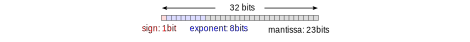
\includegraphics[width=1\linewidth]{figures/bits_single_precision.pdf}
\end{center}
$p=24$, $L=-126$, $U=127$
\begin{itemize}
\item Underfloat threshold = $2^{-126} \approx 10^{-38}$
\item Overflow threshold = $2^{128} \approx 10^{38}$
\end{itemize}

\item \textit{Double precision} (64 bits = 8 bytes) \lstinline{np.float64}
\begin{center}
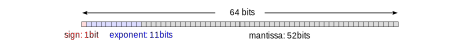
\includegraphics[width=1\linewidth]{figures/bits_double_precision.pdf}
\end{center}
$p=53$, $L=-1022$, $U=1023$
\begin{itemize}
\item Underfloat threshold = $2^{-1022} \approx 10^{-308}$
\item Overflow threshold = $2^{1024} \approx 10^{308}$
\end{itemize} 
\end{itemize}
\end{frame}

%%%%%%%%%%%%%%%%%%%%%%%%%%%%%%%%%%%%%%%%%%%%%%%%%%%%%%%%%%%%%%%%%%

\begin{frame}
\frametitle{Special values}
\textbf{Representation in IEEE 754 Standard}
\begin{itemize}
\item The number zero
$$
\texttt{s000 0000 0000 0000 0000 0000 0000 0000}
$$
$s$ = sign bit $\Rightarrow$ $+0$ ($s=1$) and $-0$ ($s=0$).
\item \texttt{NaN} (``not a number'') = result of invalid operations
$$
\texttt{s111 1111 1xxx xxxx xxxx xxxx xxxx xxxx}
$$ 
$x$ = any non-zero number, sign $s$ usually ignored
\item Infinity ($\pm\infty$)
$$
\texttt{s111 1111 1000 0000 0000 0000 0000 0000}
$$
\end{itemize}
\end{frame}

%%%%%%%%%%%%%%%%%%%%%%%%%%%%%%%%%%%%%%%%%%%%%%%%%%%%%%%%%%%%%%%%%%

\begin{frame}
\frametitle{Machine epsilon}
\textbf{Gaps between numbers in $\mathbb{F}$}
$$
x = \pm \left(d_0 + d_1\beta^{-1} + d_2\beta^{-1} + \dots+d_{p-1}\beta^{1-p}\right)\cdot\beta^E
$$
\begin{center}
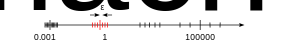
\includegraphics[width=\linewidth]{figures/floating_point_spacing.pdf}
\end{center}
$E$ $\Rightarrow$ $[2^E,2^{E+1}]$ discretised into $2^{p-1}$ pieces of size $2^{1-p}\cdot 2^E$\\[2ex]
\textbf{Machine epsilon} $E=0$ $\Rightarrow$ gap of numbers around $1$
$$
\varepsilon_{\text{mach}} := 2^{1-p} = \begin{cases}
2^{-23} \approx 10^{-7} & \text{in single precision}\\
2^{-52} \approx 2\cdot 10^{-16} & \text{in double precision}
\end{cases}
$$
\end{frame}

%%%%%%%%%%%%%%%%%%%%%%%%%%%%%%%%%%%%%%%%%%%%%%%%%%%%%%%%%%%%%%%%%%

\begin{frame}
\frametitle{Machine epsilon}
\textbf{Alternative definitions}
\begin{itemize}
\item \textit{``Gap of numbers around $1$''}
$$
\varepsilon_{\text{mach}} = 2^{1-p}
$$
\item \textit{``Smallest positive number $x\in \mathbb{F}$ that can be added to $1$ such that (after rounding to $\mathbb{F}$) the result differs from $1$''}
$$
\varepsilon_{\text{mach}} := \min_{x\in\mathbb{F},x>0}\{x: \mathcal{R}_{\mathbb{F}}(1+x)\neq 1\}
$$
\item \textit{``Relative size of rounding errors or the relative accuracy of floating point operations.''}
$$
\frac{|\mathcal{R}_{\mathbb{F}}(z)-z|}{|z|} \sim \varepsilon_{\text{mach}}.
$$
\end{itemize}
{\footnotesize NB: sometimes $\varepsilon_{\text{mach}}$ is defined with an additional factor $2$ in the literature.}
\end{frame}

%%%%%%%%%%%%%%%%%%%%%%%%%%%%%%%%%%%%%%%%%%%%%%%%%%%%%%%%%%%%%%%%%%

\begin{frame}
\frametitle{Rounding errors}
\textbf{Example 1} (harmless)
\begin{xalignat*}{2}
x&=4.7\cdot 10^{-16}\in\mathbb{F},& y&=2.9\cdot 10^{-16}\in\mathbb{F}
\end{xalignat*}
$$
z=x-y=1.8\cdot 10^{-16} = \mathcal{R}_{\mathbb{F}}(z) \in\mathbb{F}
$$
$$
\frac{\mathcal{R}_{\mathbb{F}}(z)-z}{z} = \frac{x-y-z}{z} = \frac{(4.7 -2.9 - 1.8)\cdot10^{-16}}{1.8\cdot 10^{-16}} = 0.
$$
$\Rightarrow$ small (zero) relative error if $x\sim y \sim x-y$
\end{frame}

%%%%%%%%%%%%%%%%%%%%%%%%%%%%%%%%%%%%%%%%%%%%%%%%%%%%%%%%%%%%%%%%%%

\begin{frame}
\frametitle{Rounding errors}
\textbf{Example 2} (subtracting two numbers that are very close)
\begin{xalignat*}{2}
x&=4.7\cdot 10^{-16}\in\mathbb{F},& y&=2.9\cdot 10^{-16}\in\mathbb{F}
\end{xalignat*}
\begin{xalignat*}{3}
x'&=1+x,& y'&=1+y,& z'&=x'-y'
\end{xalignat*}
In exact arithmetic: $z'=x'-y'=x-y$, but
$$
\begin{aligned}
\mathcal{R}_{\mathbb{F}}(x')&=1.00000000000000044\\
\mathcal{R}_{\mathbb{F}}(y')&=1.00000000000000022
\end{aligned}
$$
The \textbf{relative error} of $z'$
$$
\begin{aligned}
\frac{\mathcal{R}_{\mathbb{F}}(z')-z}{z} &= \frac{\mathcal{R}_{\mathbb{F}}(x')-\mathcal{R}_{\mathbb{F}}(y')-z}{z}\\
&= \frac{(4.4 - 2.2 - 1.8)\cdot10^{-16}}{1.8\cdot 10^{-16}} = \frac{0.4}{1.8} \approx 23\%
\end{aligned}
$$
Observe: $z'\ll x'\sim y'$ in contrast to $z\ll x\sim y$ (Example 1)
\end{frame}

%%%%%%%%%%%%%%%%%%%%%%%%%%%%%%%%%%%%%%%%%%%%%%%%%%%%%%%%%%%%%%%%%%

\begin{frame}
\frametitle{Rounding errors}
\textbf{Example 3} (adding two numbers of very different size)\\[1ex]
Linear system
$$
\begin{pmatrix}
0 & 1 \\ 1 & 1 
\end{pmatrix}
\begin{pmatrix}
x_0 \\ x_1
\end{pmatrix}
=
\begin{pmatrix}
1 \\ 0
\end{pmatrix}
\qquad\text{$\Rightarrow$ solution: $x_0=-1$, $x_1=1$}
$$
perturbed problem
$$
\begin{pmatrix}
-10^{-20} & 1 \\ 1 & 1 
\end{pmatrix}
\begin{pmatrix}
x_0 \\ x_1
\end{pmatrix}
=
\begin{pmatrix}
1 \\ 0
\end{pmatrix}
$$
Solution
\begin{xalignat*}{2}
  x_0&=-\frac{1}{1+10^{-20}}\approx -1,&
  x_1&=\frac{1}{1+10^{-20}}\approx 1
\end{xalignat*}
\end{frame}

%%%%%%%%%%%%%%%%%%%%%%%%%%%%%%%%%%%%%%%%%%%%%%%%%%%%%%%%%%%%%%%%%%

\begin{frame}
\frametitle{Rounding errors}
\textbf{Solution of perturbed problem}
$$
\begin{aligned}
-10^{-20} x_0 + x_1 &= 1\quad (\dagger)\\
x_0 + x_1 &= 0\quad (\star)
\end{aligned}
$$
$10^{20}\cdot (\dagger ) + (\star)$
$$
\begin{aligned}
-10^{-20} x_0 + x_1 &= 1\\
\underbrace{(1+10^{20})}_{\approx 10^{20}} x_1 &= 10^{20}
\end{aligned}
$$
$\Rightarrow$ in double precision arithmetic
$$
\begin{aligned}
-10^{-20} x_0 + x_1 &= 1\\
10^{20} x_1 &= 10^{20},
\end{aligned}
$$
$$
\Rightarrow \quad x_1 = 1 \quad \Rightarrow\quad  x_1 = 1 -10^{-20} x_0 + 1 = 1 \quad \Rightarrow \quad x_0 = 0
$$
Not close to solution $x_0=-1$, $x_1=1$ of unperturbed system!
\end{frame}

%%%%%%%%%%%%%%%%%%%%%%%%%%%%%%%%%%%%%%%%%%%%%%%%%%%%%%%%%%%%%%%%%%

\begin{frame}
\frametitle{Rounding errors}
\textbf{Fix}
$$
\begin{aligned}
-10^{-20} x_0 + x_1 &= 1\quad (\dagger)\\
x_0 + x_1 &= 0\quad (\star)
\end{aligned}
$$
$(\star ) - (\dagger)$
$$
\begin{aligned}
\underbrace{(1+10^{-20})}_{\approx 1} x_0 &= -1\\
x_0 + x_1 &= 0
\end{aligned}
$$
\begin{xalignat*}{2}
\Rightarrow \quad x_0 &= -1, & x_1 &= 1
\end{xalignat*}
This is what \lstinline{numpy.linalg.solve()} will do
\end{frame}

%%%%%%%%%%%%%%%%%%%%%%%%%%%%%%%%%%%%%%%%%%%%%%%%%%%%%%%%%%%%%%%%%%

\begin{frame}
\frametitle{Rounding errors}
\textbf{Example 4} (ill-conditioned matrix)\\[1ex]
Solve $A\boldsymbol{u}=\boldsymbol{b}$
$$
\begin{aligned}
A &= \begin{pmatrix}
1+\frac{1}{\sqrt{2}} + \frac{2+\sqrt{2}}{4}\epsilon & \frac{1}{\sqrt{2}}-\frac{\sqrt{2}}{4}\epsilon\\[1ex]
\frac{1}{\sqrt{2}}-\frac{\sqrt{2}}{4}\epsilon & 1-\frac{1}{\sqrt{2}}+\frac{2-\sqrt{2}}{4}\epsilon
\end{pmatrix}\qquad\text{$\epsilon>0$}
\\
&\approx
{\tiny%
\begin{pmatrix}
1.7071067811865475 + 0.8535533905932737 \cdot\epsilon & 0.7071067811865475 - 0.3535533905932738 \cdot\epsilon \\
0.7071067811865475 - 0.3535533905932738 \cdot\epsilon & 0.2928932188134525 + 0.1464466094067262\cdot\epsilon
\end{pmatrix}}
\end{aligned}
$$
$$
\boldsymbol{b} = \begin{pmatrix}
\frac{\sqrt{2+\sqrt{2}}+\sqrt{2-\sqrt{2}}}{2}\\[1ex]
\frac{\sqrt{2+\sqrt{2}}-\sqrt{2-\sqrt{2}}}{2}
\end{pmatrix}
\approx
{\footnotesize%
\begin{pmatrix}
1.3065629648763766\\0.5411961001461970
\end{pmatrix}}
$$
xact solution, independent of $\epsilon$
$$
\boldsymbol{u}_{\text{exact}} = 
\begin{pmatrix}
\frac{\sqrt{2 - \sqrt{2}}}{2}\\[1ex]
\frac{\sqrt{2 + \sqrt{2}}}{2}
\end{pmatrix}
\approx 
{\footnotesize%
\begin{pmatrix}
0.3826834323650897\\0.9238795325112867
\end{pmatrix}}
$$
\end{frame}

%%%%%%%%%%%%%%%%%%%%%%%%%%%%%%%%%%%%%%%%%%%%%%%%%%%%%%%%%%%%%%%%%%

\begin{frame}[fragile]
\frametitle{Rounding errors}

\begin{minipage}{0.45\linewidth}
\begin{lstlisting}
u = np.linalg.solve(A,b)
\end{lstlisting}
\end{minipage}
\hfill
\begin{minipage}{0.45\linewidth}
$\boldsymbol{u}_{\text{exact}} 
\approx 
{\footnotesize%
\begin{pmatrix}
0.3826834323650897\\0.9238795325112867
\end{pmatrix}}$
\end{minipage}\\
 \begin{center}
  \renewcommand{\arraystretch}{1.5}
\begin{tabular}{cccc}  
  \hline
$\epsilon$ & solution $\boldsymbol{u}$ & $\frac{\|\boldsymbol{u}-\boldsymbol{u}_{\text{exact}}\|_2}{\|\boldsymbol{u}_{\text{exact}}\|_2}$ & $\text{cond}(A)$\\
\hline\hline
  $10^{-3}$ & ${\tiny\begin{pmatrix}0.3826834323650560 \\ 0.9238795325113685\end{pmatrix}}$ &  $8.8408\cdot 10^{-14}$  & $4\cdot 10^3$ \\
  $10^{-6}$ & ${\tiny\begin{pmatrix}0.3826834323171860 \\0.9238795326269368\end{pmatrix}}$ & $1.2518\cdot 10^{-10}$ & $4\cdot 10^6$ \\
  $10^{-9}$ & ${\tiny\begin{pmatrix}0.3826834290672392 \\0.9238795404730024\end{pmatrix}}$ & $8.6177\cdot 10^{-9}$ & $4\cdot 10^9$ \\
  $10^{-12}$ & ${\tiny\begin{pmatrix}0.3826776593455781 \\ 0.9238934698132879\end{pmatrix}}$ & $1.5086\cdot10^{-5}$ & $4\cdot 10^{12}$ \\
  $10^{-15}$ & ${\tiny\begin{pmatrix}0.3888090807546386 \\0.9090909090909092\end{pmatrix}}$ & $1.6007\cdot10^{-2}$ & $4\cdot 10^{15}$ \\
  $8\cdot 10^{-16}$ & ${\tiny\begin{pmatrix} 0.2919799363037854 \\1.1428571428571428\end{pmatrix}}$ & $2.3702\cdot 10^{-1}$ & $5\cdot 10^{15}$ \\
  $4\cdot 10^{-16}$ & ${\tiny\begin{pmatrix} -0.0630602600160104 \\ 2.0000000000000000\end{pmatrix}}$ & $1.1648$ & $10^{16}$ \\
  \hline
\end{tabular}
\end{center}
condition number $\text{cond}(A) = \lambda_+/\lambda_-\approx 4/\epsilon$
\end{frame}

%%%%%%%%%%%%%%%%%%%%%%%%%%%%%%%%%%%%%%%%%%%%%%%%%%%%%%%%%%%%%%%%%%

\begin{frame}
\frametitle{Backward error analysis}
Solution $\boldsymbol{u}\in\mathbb{R}^n$ in exact arithmetic satisfies
$$
A\boldsymbol{u} = \boldsymbol{b}
$$
Rounding errors $\Rightarrow$ computed solution $\boldsymbol{u}'=\boldsymbol{u}+\delta\boldsymbol{u}$ solves
$$
(A+\delta A)(\boldsymbol{u}+\delta\boldsymbol{u}) = \boldsymbol{b} + \delta\boldsymbol{b}
\qquad\text{\footnotesize(assume $\delta\boldsymbol{b}=0$ for simplicity)}
$$
Goal: derive \textbf{bound} on $\delta\boldsymbol{u}$ \\[1ex]
\end{frame}

%%%%%%%%%%%%%%%%%%%%%%%%%%%%%%%%%%%%%%%%%%%%%%%%%%%%%%%%%%%%%%%%%%

\begin{frame}
\frametitle{Backward error analysis}
\textbf{Norms}
$$
\begin{aligned}
\|\boldsymbol{w}\|_\infty &:= \max_{i=0,\dots,n-1} |w_i|,\\
\|A\|_\infty &:= \max_{\boldsymbol{w}\in\mathbb{R}^n,\boldsymbol{w}\neq \boldsymbol{0}} \frac{\|A\boldsymbol{w}\|_\infty}{\|\boldsymbol{w}\|_\infty} = \max_{0\le i < n} \sum_{j=0}^{n-1} |A_{ij}|
\end{aligned}
$$
$\Rightarrow$ $\|A\boldsymbol{w}\|_\infty\le \|A\|_\infty\|\boldsymbol{w}\|_\infty$ and $\|AB\|_\infty\le\|A\|_\infty\|B\|_\infty$.
\end{frame}

%%%%%%%%%%%%%%%%%%%%%%%%%%%%%%%%%%%%%%%%%%%%%%%%%%%%%%%%%%%%%%%%%%

\begin{frame}
\frametitle{Backward error analysis}
Condition number of matrix $A$
$$
\text{cond}(A) := \|A^{-1}\|_\infty\|A\|_\infty.
$$
($=\lambda_{\text{max}}/\lambda_{\text{min}}$ for real-valued SPD matrix)\\[2ex]
\textbf{Theorem 1}\\
If the $n\times n$ matrix $A$ is non-singular and if $\delta A$ is sufficiently small
$$
\|\delta A\|_{\infty} \|A^{-1}\|_\infty \le \frac{1}{2}
$$
then $A+\delta A$ is non-singular and
$$
\frac{\|\delta\boldsymbol{u}\|_\infty}{\|\boldsymbol{u}\|_\infty} \le 2\;\text{cond}(A) \frac{\|\delta A\|_\infty}{\|A\|_\infty}
$$
Proof (not examinable): see lecture notes
\end{frame}

%%%%%%%%%%%%%%%%%%%%%%%%%%%%%%%%%%%%%%%%%%%%%%%%%%%%%%%%%%%%%%%%%%

\begin{frame}
\frametitle{Backward error analysis}
Gaussian elimination
$$
\frac{\|\delta A\|_\infty}{\|A\|_\infty} \le n\cdot \varepsilon_{\text{mach}}\cdot G(A),
$$
$G(A)$ = "well-behaved" number\\[2ex]

\textbf{Theorem 2}\\
Under the conditions of Theorem 1 and if Gaussian elimination is used to solve the linear system, the error $\delta \boldsymbol{u}$ can be bounded

$$
\frac{\|\delta\boldsymbol{u}\|_\infty}{\|\boldsymbol{u}\|_\infty} \le 2\cdot G(A)\cdot n\cdot \text{cond}(A)\cdot \varepsilon_{\text{mach}}
$$
proportional to
\begin{itemize}
\item  machine epsilon $\varepsilon_{\text{mach}}$
\item problem size $n$
\item condition number $\text{cond}(A)$
\end{itemize}
\end{frame}

%%%%%%%%%%%%%%%%%%%%%%%%%%%%%%%%%%%%%%%%%%%%%%%%%%%%%%%%%%%%%%%%%%

\begin{frame}
\frametitle{Estimating the error}
Generally impossible to compute the error $\delta\boldsymbol{u}=\boldsymbol{u}'-\boldsymbol{u}$\\[1ex]
\textbf{Residual}
$$
\boldsymbol{r}:=\boldsymbol{b}-A\boldsymbol{u}'=A\delta\boldsymbol{u} \qquad\text{($= 0$ if $\delta\boldsymbol{u}=0$)}
$$
Unfortunately
$$
\|\boldsymbol{r}\|_\infty\ll 1 \quad\nRightarrow\quad \|\delta\boldsymbol{u}\|_\infty\ll 1
$$
Properties of $\|\cdot\|_\infty$
\begin{xalignat*}{2}
\|\boldsymbol{b}\|_\infty &\le \|A\|_\infty \|\boldsymbol{u}\|_\infty, & \|\delta\boldsymbol{u}\|_\infty &\le \|A^{-1}\|_\infty \|\boldsymbol{r}\|_\infty
\end{xalignat*}
$$
\Rightarrow\quad\frac{\|\delta \boldsymbol{u}\|_\infty}{\|\boldsymbol{u}\|_\infty} 
\le \|A^{-1}\|_\infty\| \boldsymbol{r}\|_\infty \frac{\|A\|_\infty}{\|\boldsymbol{b}\|_\infty} = \text{cond}(A)\frac{\|\boldsymbol{r}\|_\infty}{\|\boldsymbol{b}\|_\infty}
$$
In the absence of any other information $\|\boldsymbol{r}\|_\infty$ is a useful quantity to measure.
\end{frame}

%%%%%%%%%%%%%%%%%%%%%%%%%%%%%%%%%%%%%%%%%%%%%%%%%%%%%%%%%%%%%%%%%%

\begin{frame}
\frametitle{Error for finite element problem}
Recall: $A^{(h)}\vec{u}^{(h)}=\vec{b}^{(h)}$ on $\widehat{K}$\\[2ex]
\begin{minipage}{0.475\linewidth}
\begin{center}
\includegraphics[width=\linewidth]{figures/error_reference_triangle.png}\\\textcolor{white}{X}
\end{center}
\end{minipage}
\hfill
\begin{minipage}{0.475\linewidth}
\begin{center}
\includegraphics[width=\linewidth]{figures/conditioning_reference_triangle.png}\\
$n_{\text{dof}}\cdot \text{cond}(A^{(h)})$
\end{center}
\end{minipage}\\
Typical problem in Scientific Computing
\begin{itemize}
\item Large $n_{\text{dof}} \gg 1$
\item Ill-conditioned $\text{cond}(A^{(h)})$
\end{itemize}
\end{frame}

%%%%%%%%%%%%%%%%%%%%%%%%%%%%%%%%%%%%%%%%%%%%%%%%%%%%%%%%%%%%%%%%%%

\section{Unstructured meshes}

%%%%%%%%%%%%%%%%%%%%%%%%%%%%%%%%%%%%%%%%%%%%%%%%%%%%%%%%%%%%%%%%%%

\begin{frame}
  \tableofcontents[currentsection]
\end{frame}


%%%%%%%%%%%%%%%%%%%%%%%%%%%%%%%%%%%%%%%%%%%%%%%%%%%%%%%%%%%%%%%%%%

\end{document}

# Unstructured meshes
So far, we have only solved our model PDE on a very simple domain, consisting of a single reference triangle. We now discuss how to extend the finite element approach to more general domains, using the concepts introduced in [[CH24]](https://finite-element.github.io/3_meshes.html#mesh-entities). Assume that we want to solve the PDE on a $d$-dimensional manifold $\Omega\subset \mathbb{R}^D$ that is embedded in $D$ dimensional space. For example, we might want to solve it in a rectangular domain or on the surface of a sphere. The manifold is then approximated by a *mesh*, which can be described as a collection of topological entities. For example, if $d=2$, the mesh will consist of zero-dimensional vertices, one-dimensional edges and two-dimensional triangular cells (although it is also possible to use more general polygonal cells we do not consider this here). In general, the co-dimension $c$ of a $d'$-dimensional mesh entity is given by $c=d-d'$. In the following we will only consider the case $d=D=2$, but the central ideas that are developed in the following also apply to more complicated setups. For $d=D=2$ we have:

| topological entity  | dimension $d'$ | co-dimension $c$ |
| ------------------- | -------------- | ---------------- |
| cell (triangle) $K$ | $2$            | $0$              |
| facet (edge) $F$    | $1$            | $1$              |
| vertex (point) $v$  | $0$            | $2$              |

 @fig:triangular_mesh shows a two-dimensional mesh with $n_{\text{vertex}}=6$ vertices, $n_{\text{facet}}=10$ facets and $n_{\text{cell}}=5$ cells in which all topological entities are labelled by their co-dimension and a unique number that can later be used to identify the entity.

![:fig:triangular_mesh: simple triangular mesh](figures/simple_mesh.svg)

## Topology
The mesh topology describes which entities are connected to which other entities. For example, each cell has exactly three facets and each facet is defined by exactly two vertices, and the topology tells us which specific facets/vertices these are: in the example above, cell $(0,1)$ has the facets $(1,3), (1,2), (1,5)$ and facet $(1,2)$ has the endpoints $(2,1), (2,2)$.

More generally, this information can be encoded in two matrices: An $n_{\text{cell}}\times 3$ matrix $I^{K\rightarrow F}$ which describes which facets bound each cell

$$
I^{K\rightarrow F}_{\alpha\beta} = \text{index of $\beta$-th facet of cell $\alpha$}
$$

and an $n_{\text{facet}}\times 2$ matrix $I^{F\rightarrow v}$ which describes what the endpoints of each facet are

$$
I^{F\rightarrow v}_{\beta\gamma} = \text{index of $\gamma$-th vertex of facet $\beta$}.
$$

Note that there is some freedom as to how we number the facets associated each cell; the numbering we adopt here is one in which for each cell $\alpha$ the facets with indices $I^{K\rightarrow F}_{\alpha0}$, $I^{K\rightarrow F}_{\alpha1}$ and $I^{K\rightarrow F}_{\alpha2}$ are arranged in a counter-clockwise fashion (note that there are three possible orderings that satisfy this condition, so we have to pick one). Similarly, we adapt an ordering of the vertices associated with each facet such that for each facet $\beta$ we have that $I^{F\rightarrow v}_{\beta0} < I^{F\rightarrow v}_{\beta1}$; in @fig:triangular_mesh this is indicated by the arrows on the edges.

For convenience, we can also use $I^{K\rightarrow F}$ and $I^{F\rightarrow v}$ to construct the $n_{\text{cell}}\times 3$ matrix $I^{K\rightarrow v}$ which describes the vertices of a given cell

$$
I^{K\rightarrow v}_{\alpha\gamma} = \text{index of $\gamma$-th vertex of cell $\alpha$}.
$$

In each cell $\alpha$, we number the vertices in a counter-clockwise fashion such that the $\gamma$-th vertex lies opposite the $\gamma$-the facet of the cell. Mathematically, this can be expressed as

$$
\begin{aligned}
I^{K\rightarrow v}_{\alpha\gamma} \not\in \{I^{F\rightarrow v}_{\beta0},I^{F\rightarrow v}_{\beta1}\}\quad\text{for $\beta =I^{K\rightarrow F}_{\alpha\gamma}$}
\end{aligned}.
$$

Note that the counter-clockwise numbering of the facets and vertices in each cell is consistent with the numbering of unknowns on the reference triangle in @fig:reference_triangle.

For example, the matrices $I^{K\rightarrow F}$, $I^{F\rightarrow v}$ and $I^{K\rightarrow v}$ for the simple mesh shown above are given by

$$
\begin{aligned}
I^{K\rightarrow F} &= \begin{pmatrix}
0 & 3 & 1 & 0 & 3 \\
1 & 2 & 2 & 9 & 6 \\
8 & 5 & 7 & 5 & 4
\end{pmatrix}^{\top}\\
I^{F\rightarrow v} &= \begin{pmatrix}
0 & 1 & 1 & 2 & 2 & 1 & 3 & 2 & 0 & 0 \\
1 & 4 & 2 & 5 & 3 & 5 & 5 & 4 & 4 & 5
\end{pmatrix}^{\top}\\
I^{K\rightarrow v} &= \begin{pmatrix}
4 & 1 & 2 & 5 & 3 \\
0 & 5 & 4 & 1 & 2 \\
1 & 2 & 1 & 0 & 5
\end{pmatrix}^{\top}
\end{aligned}
$$

You should convince yourself that these matrices satisfy the conditions outlined above.

 @fig:rectangle_mesh shows another example (created with `rectangle_mesh(Lx=1.0, Ly=1.0, nref=1)`, see below). The global indices of vertices, facets and cells are plotted separatedly. The figure in the lower right corner illustrates how the global indices are related to the local indices of the reference cell.

![:fig:rectangle_mesh: Numbering of topological entities on a rectangle mesh](figures/rectangle_mesh.svg)

Referring to the local numbering of facets and vertices in the lower right plot we read off:

$$
\begin{aligned}
I^{K\rightarrow F} &= \begin{pmatrix}
5 & 1 & 2 & 10 & 8 & 0 & 7 & 13\\
0 & 3 & 4 & 11 & 1 & 6 & 9 & 14\\
11 & 12 & 10 & 12 & 14 & 15 & 13 & 15
\end{pmatrix}^{\top}
\\
I^{F\rightarrow v} &= \begin{pmatrix}
1 & 2 & 0 & 2 & 0 & 1 & 1 & 3 & 2 & 3 & 5 & 4 & 4 & 7 & 4 & 4\\
4 & 4 & 5 & 5 & 6 & 6 & 7 & 7 & 8 & 8 & 6 & 6 & 5 & 8 & 8 & 7
\end{pmatrix}^{\top}
\\
I^{K\rightarrow v} &= \begin{pmatrix}
4 & 5 & 6 & 4 & 4 & 7 & 8 & 4\\
6 & 4 & 5 & 5 & 8 & 4 & 7 & 7\\
1 & 2 & 0 & 6 & 2 & 1 & 3 & 8
\end{pmatrix}^{\top}
\end{aligned}
$$

Again, convince yourself that these matrices are consistent with the conditions we imposed on the numbering.

### Implementation
The abstract class `Mesh` in [fem/mesh.py](https://github.com/eikehmueller/finiteelements/blob/main/src/fem/mesh.py) encodes the mesh topology. It has the following members:

* properties `ncells`, `nfacets` and `nvertices` which give the total number of cells ($=n_{\text{cell}}$), facets ($=n_{\text{facet}}$) and vertices ($=n_{\text{vertex}}$) respectively
* `cell2facet`: a nested list such that `cell2facet[alpha][beta]` $= I^{K\rightarrow F}_{\alpha\beta}$
* `facet2vertex`: a nested list such that `facet2vertex[beta][gamma]` $= I^{F\rightarrow v}_{\beta\gamma}$
* `cell2vertex`: a nested list such that `cell2vertex[alpha][gamma]` $= I^{K\rightarrow v}_{\alpha\gamma}$. Since $I^{K\rightarrow v}_{ik}$ can be derived from $I^{K\rightarrow F}_{\alpha\beta}$ and $I^{F\rightarrow v}_{\beta\gamma}$, `cell2vertex` is implemented as a [`@functools.cached_property`](https://docs.python.org/3/library/functools.html#functools.cached_property).
* an array `coordinates` of shape $(n_{\text{vertex}},2)$ whose columns contain the two-dimensional coordinates of the mesh vertices

The class also contains a method `refine(nref)` which can be used to construct a refined mesh from a given mesh by sub-dividing each triangle into four smaller triangles.

In [fem/utilitymeshes.py](https://github.com/eikehmueller/finiteelements/blob/main/src/fem/utilitymeshes.py) two concrete classes are derived from this abstract base class:

* `rectangle_mesh(Lx=1.0, Ly=1.0, nref=0)` is a triangulation of the domain $[0,L_x]\times[0,L_y]$ with a given number of refinements $n_{\text{ref}}$. The number of cells is $n_{\text{cells}} = 2^{n_{\text{ref}}+1}$
* `triangle_mesh(corners=None, nref=0)` is a triangulation of the domain triangle defined by the array `corners` (if this is `None`, the reference triangle us used) with a given number of refinements $n_{\text{ref}}$. The number of cells is $n_{\text{cells}} = 2^{n_{\text{ref}}}$

## Geometry
Observe that so far we have only discussed the **topology** of the mesh and we have not said anything about its **geometry**, i.e. where exactly the topological entities are located in space. To do this, we first discuss how we can associate data with the mesh and then use this to encode its geometry.

# Function spaces
## Grid cells and reference elements
We now construct a function space $\mathcal{V}_h\subset H^1(\Omega_h)$ on the domain $\Omega_h$ defined by the mesh as follows. First, we assume that each cell $K$ of the mesh is the image of the reference cell $\widehat{K}$ under a bijective map $X_K:\widehat{K}\rightarrow K\subset \Omega\subset \mathbb{R}^2$: for each $\widehat{x}\in\widehat{K}$ there is exactly one point $x=X_K(\widehat{x})\in K$ and vice versa. For an arbitrary real-valued function $f:K\rightarrow \mathbb{R}$ we define the *pullback* $\widehat{f}:\widehat{K}\rightarrow \mathbb{R}$ under $X_K$ as

$$
\widehat{f} = f\circ X_K
$$

i.e.

$$
\widehat{f}(\widehat{x}) = f(X_K(\widehat{x}))\qquad\text{for all $\widehat{x}\in\widehat{K}$}.
$$


Next, assume that in each grid cell $K$ the pullback of the function $u|_K$ under the map $X_K$ is a polynomial. More specifically we define
$$
\mathcal{V}_h := \{u\in H^1(\Omega_h): u|_K(x) = \widehat{u}_K(\widehat{x})\quad \text{for some $\widehat{u}_K\in\mathcal{P}_p(\widehat{K})$ with $x=X_K(\widehat{x})$ for all cells $K\in\Omega_h$}\}.
$$

![:fig:pullback: pullback to reference element](figures/reference_mapping.svg)

We can now use the basis of $\mathcal{P}_p(\widehat{K})$ that we constructed in one of the previous lectures to represent the functions $\widehat{u}_K$. However, care has to be taken to ensure that the function $u\in\mathcal{V}_h$ defined on the entire domain is continuous across facets and at the vertices. To guarantee this, we need to think carefully about the arrangement of unknowns on the mesh.

For this, recall that any function $u_h$ in the function space $\mathcal{V}_h$ can be written as

$$
u_h(x) = \sum_{\ell_{\text{global}}=0}^{n-1} u^{(h)}_{\ell_{\text{global}}} \Phi^{(h)}_{\ell_{\text{global}}}(x)
$$

where the $\Phi^{(h)}_{\ell_{\text{global}}}$ are the *global* basis functions and $u^{(h)}_{\ell_{\text{global}}}$ are entries of the *global* dof-vector $\boldsymbol{u}^{(h)}$. To ensure continuity of $u_h$ we need to associate the indices $\ell_{\text{global}}$ with the correct mesh entities.

### Arrangement of unknowns
Assume that we have a finite element with $\nu_{\text{vertex}}$ unknowns per vertex, $\nu_{\text{facet}}$ unknowns per facet and $\nu_{\text{interior}}$ unknowns per cell. 
Let $N_{\text{vertex}} = n_{\text{vertex}}\cdot \nu_{\text{vertex}}$, $N_{\text{facet}} = n_{\text{facet}}\cdot \nu_{\text{facet}}$ and $N_{\text{interior}} = n_{\text{cell}}\cdot \nu_{\text{interior}}$ be the total number of unknowns associated with vertices, facets and cell interiors respectively.

We number the unknowns by using the first $N_{\text{vertex}}$ indices for unknowns associated with vertices, the next $N_{\text{facet}}$ indices for unknowns associated with facets and the remaining $N_{\text{interior}}$ indices for unknowns associated with cell interiors. More specifically:

* unknowns with indices $\ell_{\text{global}}\in\{\gamma\cdot \nu_{\text{vertex}},\dots,(\gamma+1)\cdot \nu_{\text{vertex}}-1\}$ are associated with the $\gamma$-th vertex
* unknowns with indices $\ell_{\text{global}}\in\{N_{\text{vertex}}+\beta\cdot \nu_{\text{facet}},\dots,N_{\text{vertex}}+(\beta+1)\cdot \nu_{\text{facet}}-1\}$ are associated with the $\beta$-th facet
* unknowns with indices $\ell_{\text{global}}\in\{N_{\text{vertex}}+N_{\text{facet}}+\alpha\cdot \nu_{\text{interior}},\dots,N_{\text{vertex}}+N_{\text{facet}}+(\alpha+1)\cdot \nu_{\text{interior}}-1\}$ are associated with the $\alpha$-th cell

The facet-unknowns are ordered along the orientation of each edge.

@fig:triangular_mesh_with_unknowns shows an example for the $p=3$ Lagrange element. For this mesh there are $N_{\text{vertex}}=6$ unknowns associated with the vertices, $N_{\text{facet}}=10\cdot 2=20$ unknowns associated with the facets and $N_{\text{interior}} = 5$ unknowns associated with the cell interiors.

![:fig:triangular_mesh_with_unknowns: simple triangular mesh with unknowns](figures/simple_mesh_with_dof_numbers.svg)

### Local-to-global map
When we introduced the concept of a finite element, we only considered *local* basis functions $\phi_\ell$. Since the functions in $\mathcal{V}_h$ are continuous, the global basis functions $\Phi^{(h)}_{\ell_{\text{global}}}$ are a combination of local basis functions: for example, global functions associated with a vertex are a combination of local basis functions on the cells that touch this vertex. Hence, in general the dof-index $\ell_{\text{global}}$ is related to several pairs $(\alpha,\ell)$ of cell indices $\alpha$ and local dof-indices $\ell$.

Conversely, on each cell with index $\alpha$ we need to map the $\ell$-th local dof-index to the global dof-index $\ell_{\text{global}}$. Note that this map is surjective but not injective since the unknowns associated with the facets and vertices are shared.

The map $(\alpha,\ell) \mapsto \ell_{\text{global}}$ is realised in two steps:

1. For the given $\ell$, we first work out the entity-type $E$ (cell, facet or vertex) it is associated with, as well as the index $\rho$ of this entity on the reference triangle and the index $j$ of the dof on that reference entity. Recall that for the finite element we have the dof-map $\mu_{\text{dof}}$ that $\ell = \mu_{\text{dof}}(E,\rho,j)$, so we can obtain $E$, $\rho$ and $j$ from the inverse of this map, which is implemented as the `inverse_dofmap()` method in the `FiniteElement` base class in [`fem/finiteelement.py`](https://github.com/eikehmueller/finiteelements/blob/main/src/fem/finiteelement.py).
2. Next, we map the tuple $(E,\rho,j)$ to the global dof index $\ell_{\text{global}}$ taking into account the arrangement of unknowns described above:
   1. If $E=\text{vertex}$: $\ell_{\text{global}} = \gamma\cdot \nu_{\text{vertex}}+j$ where $\gamma=I^{K\rightarrow v}_{\alpha\rho}$ is the global index of the vertex with local index $\rho$.
   2. If $E=\text{facet}$: $\ell_{\text{global}} = N_{\text{vertex}}+\beta\cdot \nu_{\text{facet}}+\widetilde{j}$ where $\beta=I^{K\rightarrow F}_{\alpha\rho}$ is the global index of the facet with local index $\rho$. Note that the orientation of the facet does not necessarily match the orientation on the reference element $\widehat{K}$. To take this into account, set $\widetilde{j}=j$ if the orientations agree and set $\widetilde{j} = \nu_{\text{facet}}-1-j$ otherwise.
   3. If $E=\text{cell}$: $\ell_{\text{global}} = N_{\text{vertex}}+N_{\text{facet}}+\alpha\cdot \nu_{\text{interior}}+j$ ($\rho$ is ignored in this case)

## Implementation in Python

### Function spaces

The necessary functionality is implemented in the `FunctionSpace` class in [`fem/functionspace.py`](https://github.com/eikehmueller/finiteelements/blob/main/src/fem/functionspace.py). The initialiser is passed a `mesh` and a `finiteelement` and the class provides the following functionality:

* The property `ndof` contains the total number of unknowns in the function space
* The method `local2global(self, alpha, ell)` implements the map $(\alpha,\ell)\mapsto\ell_{\text{global}}$ described above. If the parameter `ell` is a single integer index in the range $0,1,\dots,\nu-1$, the method returns a single number $\ell_{\text{global}}$. If `ell` is an [iterable](https://docs.python.org/3/glossary.html#term-iterable) (such as a list `[0,3,4]` or `range(1,6,2)`) the global index will be computed for each local index and the method returns a list.

### Functions
To store functions in a given function space, the class `Function` in [`fem/function.py`](https://github.com/eikehmueller/finiteelements/blob/main/src/fem/function.py) is provided. This initialiser of this class gets passed a `FunctionSpace` object, which it stores together with a numpy array `function.data` that contains the vector $\boldsymbol{u}^{(h)}$. This information then allows the reconstruction of the function $u_h \in \mathcal{V}_h$ given by

$$
u_h(x) = \sum_{\ell_{\text{global}}=0}^{N-1} u^{(h)}_{\ell_{\text{global}}} \Phi^{(h)}_{\ell_{\text{global}}}(x)
$$

To store *co-functions* such as $b(\cdot)\in\mathcal{V}_h^*$ with (for example)

$$
b(v) = \int_\Omega v(x) f(x)\;dx
$$

a `CoFunction` class is provided in the same file. This class is also constructed by passing it a `FunctionSpace` object, but now the `cofunction.data` array contains the vector $\boldsymbol{b}^{(h)}$ whose elements are given by

$$
b^{(h)}_{\ell_{\text{global}}} = b\left(\Phi^{(h)}_{\ell_{\text{global}}}\right).
$$

## Encoding geometry information
The geometry of the mesh is encoded in the functions $X_K$ which describe the mapping from the reference element $\widehat{K}$ to a particular cell $K$. We can combine the $X_K$ in each cell into a global function $X$ which is defined on the entire mesh. The crucial observation is now that each component of $X_K$ can be represented by a function in a finite element space $\mathcal{W}_h$ which is defined in the same way as $\mathcal{V}_h$ (but possibly with a different polynomial degree). Hence, we can define a coordinate function 

$$
X \in \mathcal{W}_h^{\times} = \mathcal{W}_h \times \mathcal{W}_h
$$
which encodes the mesh geometry. This idea is used in successful finite element libraries such as [Firedrake](https://www.firedrakeproject.org/).

The space $\mathcal{W}_h^{\times}$ is a vector function space. Let $w=(w_0,w_1):\widehat{K}\rightarrow \mathbb{R}^2$ be a vector-valued function. Then the degrees of freedom $\lambda^\times$ of $\mathcal{W}^\times_h$ are given by:

$$
\lambda^\times_{\ell^\times}(w) = \begin{cases} 
\lambda_{\ell^\times/2}(w_0) & \text{for $\ell^\times$ even}\\
\lambda_{(\ell^\times-1)/2}(w_1) & \text{for $\ell^\times$ odd}\\
\end{cases}
$$

The corresponding vector-valued nodal basis functions $\phi^\times_\ell$ which satisfy $\lambda^{\times}_{\ell^\times}(\phi^\times_{k^\times})=\delta_{\ell^\times k^\times}$ (recall @eqn:nodal_basis_definition) are
$$
\phi^\times_{\ell^\times}(x) = 
\begin{cases}
\begin{pmatrix}\phi_{\ell^\times/2}(x)\\0\end{pmatrix} & \text{for $\ell^\times$ even}\\[2ex]
\begin{pmatrix}0 \\\phi_{(\ell^\times-1)/2}(x)\end{pmatrix} & \text{for $\ell^\times$ odd}
\end{cases}
$$

### Tabulation of basis functions
As for scalar-valued function spaces we can *tabulate* the basis functions. For a given set of points $\boldsymbol{\zeta}:=\{\zeta^{(r)}\}_{r=0}^{n-1}$, we obtain the $n \times \nu^\times \times 2$ matrix $T^\times$ with

$$
T^\times_{r\ell^\times a}(\boldsymbol{\zeta}) := (\phi^\times_{\ell^\times}(\zeta^{(r)}))_a = 
\begin{cases}
\phi_{\ell^\times/2}(\zeta^{(r)}) = T_{r,\ell^\times/2}& \text{if $\ell^\times$ even and $a=0$} \\
\phi_{(\ell^\times-1)/2}(\zeta^{(r)}) = T_{r,(\ell^\times-1)/2} & \text{if $\ell^\times$ odd and $a=1$} \\
0 & \text{otherwise}
\end{cases}
$$

Furthermore, the derivatives are collected in the $n \times \nu^\times \times 2\times 2$ matrix $T^{\times\partial}$ matrix with

$$
T^{\times\partial}_{r\ell^\times ab}(\boldsymbol{\zeta}) := \frac{(\partial \phi^\times_{\ell^\times})_a}{\partial x_b}(\zeta^{(r)})  = \begin{cases}
\frac{\phi_{\ell^\times/2}}{\partial x_b}(\zeta^{(r)}) = T_{r,\ell^\times/2,b}& \text{if $\ell^\times$ even and $a=0$} \\[2ex]
\frac{\partial\phi_{(\ell^\times-1)/2}}{\partial x_b}(\zeta^{(r)}) = T_{r,(\ell^\times-1)/2,b} & \text{if $\ell^\times$ odd and $a=1$} \\[2ex]
0 & \text{otherwise}
\end{cases}
$$

### Construction of global coordinates
We can now evaluate the value of $X_K(\zeta^{(r)})$, i.e. the global coordinate for some point $\zeta^{(r)}$ inside the reference cell when mapped to the cell $K$. For this, assume that the coordinate field $X\in\mathcal{W}_h^\times$ is represented by the global dof-vector $\boldsymbol{X}$. Then 

$$
(X_K(\zeta^{(r)}))_a = \sum_{\ell^\times} \overline{X}_{\ell^\times} \left(\phi_{\ell^\times}^\times(\zeta^{(r)})\right)_a = \sum_{\ell^\times} \overline{X}_{\ell^\times} T^\times_{r\ell^\times a} 
$$

where $\overline{\boldsymbol{X}}$ is the local coordinate vector with

$$
\overline{X}_{\ell^\times} = X_{\ell^\times_{\text{global}}(\alpha,\ell^\times)}.
$$

In this expression $\ell^\times_{\text{global}}(\alpha,\ell^\times)$ is the global dof-index that corresponds to the local dof-index $\ell^\times$ in the cell with index $\alpha$.

## Implementation in Python
Vector-valued finite elements are implemented in the class `VectorElement` in [`fem/vectorelement.py`](https://github.com/eikehmueller/finiteelements/blob/main/src/fem/vectorelement.py). This is a subclass of the abstract base class `FiniteElement` (recall [`fem/finiteelement.py`](https://github.com/eikehmueller/finiteelements/blob/main/src/fem/finiteelement.py)). In its constructor it gets passed a `FiniteElement` which is used to represent each of its components. The class `VectorElement` then uses the underlying scalar-valued finite element to implement the appropriate methods for tabulating the degrees of freedom and (gradients of) the basis functions:

* `tabulate_dofs(fhat)` is passed a vector-valued function $\widehat{f}$, and returns the vector $\left(\lambda_0(\widehat{f}),\lambda_1(\widehat{f}),\lambda_2(\widehat{f}),\dots,\lambda_{\nu-1}(\widehat{f})\right)^\top\in \mathbb{R}^{\nu}$.
* `tabulate()` is passed an array of shape $n\times 2$ of points $\{\zeta^{(r)}\}_{r=0}^{n-1}$ and returns an array $T^\times$ of shape $n\times \nu\times 2$ with the basis function evaluations at these points; if only a single point is passed, it returns an array of shape $\nu\times 2$
* `tabulate_gradient()` is passed an array of shape $n\times 2$ of points $\{\zeta^{(r)}\}_{r=0}^{n-1}$ and returns an array $T^{\times\partial}$ of shape $n\times \nu\times 2\times 2$ with the basis function gradient evaluations at these points; if only a single point is passed, it returns an array of shape $\nu\times 2\times 2$ 

Looking back at the `Mesh` class in [`fem/mesh.py`](https://github.com/eikehmueller/finiteelements/blob/main/src/fem/mesh.py), observe that it has a property `mesh.coordinates`, which is a `Function` on a `FunctionSpace` over `VectorElements`. This will allow us to extract the mesh geometry.

# Global assembly
We are now ready to assemble the stiffness matrix $A^{(h)}$ and the right hand side vector $\boldsymbol{b}^{(h)}$ which define the linear system
$$
A^{(h)} \boldsymbol{u}^{(h)} = \boldsymbol{b}^{(h)}.
$$
With knowledge of the dof-vector $\boldsymbol{u}^{(h)}$ we can reconstruct the finite element solution
$$
u_h(x) = \sum_{\ell=0}^{n-1} u^{(h)}_{\ell_{\text{global}}} \Phi^{(h)}_{\ell_{\text{global}}}(x).
$$
Recall that the entries of the right hand side vector and stiffness matrix are given by
$$
b^{(h)}_{\ell_{\text{global}}}:=b(\Phi^{(h)}_{\ell_{\text{global}}})
$$
and
$$
A^{(h)}_{{\ell_{\text{global}}}{k_{\text{global}}}}:= a\left(\Phi^{(h)}_{k_{\text{global}}},\Phi^{(h)}_{\ell_{\text{global}}}\right).
$$
We now discuss the assembly of these two quantities.

## Assembly of RHS vector
Since $b(v) = \int_\Omega f(x)v(x)\;dx$ we compute the entries of the vector $b^{(h)}$ by splitting the integral over the domain $\Omega$ into the sum of integrals over the cells $K$:
$$
\begin{aligned}
b^{(h)}_{\ell_{\text{global}}} &= \int_\Omega f(x) \Phi_{\ell_{\text{global}}}(x)\;dx\\
&= \sum_{K\in \Omega_h} \int_K f(x) \Phi_{\ell_{\text{global}}}(x) \; dx\\
\end{aligned}
$$
If $\alpha$ is the index of cell $K$, we can identify the *global* index $\ell_{\text{global}}=\ell_{\text{global}}(\alpha,\ell)$ with the corresponding cell-*local* index $\ell$, transform variables to integrate over the reference cell $\widehat{K}$ and write 
$$
\begin{aligned}
b^{(h)}_{\ell_{\text{global}}} &= \sum_{K\in \Omega_h}\int_{\widehat{K}} \widehat{f}_K(\widehat{x}) \phi_\ell(\widehat{x})\;|\det{J}(\widehat{x})|\;d\widehat{x}
\end{aligned}
$$
where $\widehat{f}_K = f\circ X_K$ is the pullback of $f$ to the cell $K$, i.e. $\widehat{f}_K(\widehat{x}) :=  f(x) = f(X_K(\widehat{x}))$ for all $\widehat{x}\in\widehat{K}$. Note that for degrees of freedom which are shared between neighbouring cells, there can be contributions from different cells since several $(\alpha,\ell)$ can correspond to the same $\ell_{\text{global}}$.

Next, replace the integration by numerical quadrature and use the tabulated basis functions $T_{q\ell}=\phi_\ell(\xi^{(q)})$ to obtain
$$
\begin{aligned}
b^{(h)}_{\ell_{\text{global}}} &\approx \sum_{K\in \Omega_h} \sum_q w_q \widehat{f}_K(\xi^{(q)}) \phi_\ell(\xi^{(q)})\;|\det{J}(\xi^{(q)})|\\
&= \sum_{K\in \Omega_h} \sum_q w_q \widehat{f}_K(\xi^{(q)}) T_{q\ell}\;|\det{J}(\xi^{(q)})|.
\end{aligned}
$$
To evaluate the cell-local function $\widehat{f}_K$ at the quadrature point $\xi^{(q)}$ we need to work out the global coordinate $x_K^{(q)}=X_K(\xi^{(q)})$ which corresponds to this point and use
$$
\widehat{f}_K(\xi^{(q)}) = f(x_K^{(q)}).
$$
In each cell $x_K$ can be expanded in terms of vector-valued basis functions as
$$
(x_K^{(q)})_a = (X_K(\xi^{(q)}))_a = \sum_{\ell^\times} (\phi^\times_{\ell^\times}(\xi^{(q)}))_a X_{\ell^\times_{\text{global}}} = \sum_{\ell^\times} T^\times_{q\ell^\times a} \overline{X}_{\ell^\times}
$$
where $\ell^\times_{\text{global}}=\ell_{\text{global}}^\times(\alpha,\ell^\times)$ is the global dof-index of the coordinate field which corresponds to the cell index $i$ and the local dof-index $\ell^\times$. As before, $\overline{\boldsymbol{X}}$ is the cell-local dof-vector with $\overline{X}_{\ell^\times} = X_{\ell_{\text{global}}^\times}$.

The Jacobian is given by
$$
J_{ab}(\xi^{(q)}) = \frac{\partial (x_K^{(q)})_a }{\partial x_b} = \frac{\partial (X_K)_a }{\partial x_b}(\xi^{(q)})
= \sum_{\ell^\times} X_{\ell^\times_{\text{global}}} \frac{\partial (\phi^\times_{\ell^\times})_a }{\partial x_b}(\xi^{(q)})
= \sum_{\ell^\times} \overline{X}_{\ell^\times} T^{\times\partial}_{q\ell^\times ab}
$$
Putting everything together, we arrive at the following procedure:

**Algorithm: assembly of right-hand-side vector $\boldsymbol{b}^{(h)}$**
1. Initialise $\boldsymbol{b}^{(h)} \gets 0$
2. **For** all cells $K$ **do**:
3. $~~~~$ Extract the coordinate dof-vector $\overline{\boldsymbol{X}}$ with $\overline{X}_{\ell^\times} = X_{\ell^\times_\text{global}(\alpha,{\ell^\times})}$ where $\alpha$ is the index of cell $K$
4. $~~~~$ **For** all quadrature points $q$ **do**:
5. $~~~~~~~~$ Compute the determinant $D_q$ of the Jacobian $J(\xi^{(q)})$ with $J_{ab}(\xi^{(q)}) = \sum_{\ell^\times} \overline{X}_{\ell^\times} T^{\times\partial}_{q\ell^\times ab}$
6. $~~~~~~~~$ Compute $(x_K^{(q)})_a = \sum_{\ell^\times} T^\times_{q\ell^\times a} \overline{X}_{\ell^\times}$ and evaluate $F_q = \widehat{f}_K(\xi^{(q)})=f(x_K^{(q)})$
7. $~~~~$ **end do**
8. $~~~~$ Construct the local dof-vector $\boldsymbol{b}^{(h),\text{local}}$ with
$$b^{(h),\text{local}}_{\ell} = \sum_q w_q F_q T_{q\ell} D_q$$
1. $~~~~$ **For** all local dof-indices $\ell$ **do**:
2. $~~~~~~~~$ Increment $b_{\ell_{\text{global}}}^{(h)}\gets b_{\ell_{\text{global}}}^{(h)} + b^{(h),\text{local}}_\ell$ with $\ell_{\text{global}} = \ell_{\text{global}}(\alpha,\ell)$
3. $~~~~$ **end do**
4. **end do**

#### Illustration
@fig:global_assembly_rhs visualises the assembly of the global vector $\boldsymbol{b}^{(h)}$. The two cells have global indices $\ell_{\text{global}}=[2,4,8]$ and $\ell_{\text{global}}=[8,11,16]$ respectively. Note that both cells contribute to the global vector entry $b^{(h)}_8$.
![:fig:global_assembly_rhs: Global assembly of right hand side vector](figures/global_assembly_rhs.svg)

#### Implementation
The summation $\sum_q w_q F_q T_{q\ell} D_q$ of the local vector entries can be realised with numpy's [`einsum()`](https://numpy.org/doc/stable/reference/generated/numpy.einsum.html) method.

To insert the entries of the local vector $\boldsymbol{b}^{(h),\text{local}}$ into the global vector $\boldsymbol{b}^{(h)}$ we can use slicing notation, i.e. write
```
b_h[ell_global] += b_h_local[:]
```
where `ell_global` is the list of global dof-indices that correspond to the local dof-indices in the cell. In the code, this list can be constructed as
```
ell_global = fs.local2global(alpha,range(ndof))
```
In this expression `fs` is a `FunctionSpace` object and `ndof` is the number $\nu$ of local unknowns in each cell.

Global assembly of the right hand side vector $\boldsymbol{b}^{(h)}$ is implemented in the function `assemble_rhs(f, r, quad)` in [fem/assembly.py](https://github.com/eikehmueller/finiteelements/blob/main/src/fem/assembly.py). This method gets passed a Python function $f$, a `CoFunction` object `r` to hold the result and a quadrature rule `quad`.

## Assembly of LHS matrix
To assemble the stiffness matrix, we again split the integral into a sum of integrals over grid cells $K$:
$$
\begin{aligned}
A^{(h)}_{\ell_{\text{global}},k_{\text{global}}} &= \int_\Omega \left(\kappa \nabla \Phi^{(h)}_{k_{\text{global}}}(x) \cdot\nabla\Phi^{(h)}_{\ell_{\text{global}}}(x)+\omega \Phi^{(h)}_{k_{\text{global}}}(x)\Phi^{(h)}_{\ell_{\text{global}}}(x)\right)dx\\
&= \sum_{K\in\Omega_h}\int_K \left(\kappa \nabla \Phi^{(h)}_{k_{\text{global}}}(x) \cdot\nabla\Phi^{(h)}_{\ell_{\text{global}}}(x)+\omega \Phi^{(h)}_{k_{\text{global}}}(x)\Phi^{(h)}_{\ell_{\text{global}}}(x)\right)dx
\end{aligned}
$$
Next, we change variables in each cell to convert the integrals into integrals over the reference cell $K$. For this, note that the global basis functions and their derivatives transform as follows:
$$
\begin{aligned}
\Phi^{(h)}_{\ell_{\text{global}}}(x) &= \phi_\ell(\widehat{x})\\
\nabla \Phi^{(h)}_{\ell_{\text{global}}}(x) &= J^{-\top}(\widehat{x}) \widehat{\nabla}\phi_\ell(\widehat{x})
\end{aligned}
$$
Here $\ell_{\text{global}}=\ell_{\text{global}}(\alpha,\ell)$ is again the global dof-index that is associated with the local dof-index $\ell$ in the cell with index $\alpha$. The second identity can be easily verified by using the chain rule since $x=X_K(\widehat{x})$. With this we find
$$
\begin{aligned}
A^{(h)}_{\ell_{\text{global}},k_{\text{global}}} &= \sum_{K\in \Omega_h}\int_K \left(\kappa J^{-\top}(\widehat{x}) \widehat{\nabla} \phi_k (\widehat{x})\cdot J^{-\top}(\widehat{x})\widehat{\nabla}\phi_\ell(\widehat{x}) + \omega\phi_k(\widehat{x})\phi_\ell(\widehat{x})\right)|\det{J}(\widehat{x})|d\widehat{x}.
\end{aligned}
$$
Next, approximate the integrals by numerical quadrature and use the tabulated basis functions $T_{q\ell} = \phi_\ell(\xi^{(q)})$, $T^\partial_{q\ell a} = \frac{\partial\phi_\ell}{\partial \widehat{x}_a}(\xi^{(q)})$ to obtain
$$
\begin{aligned}
A^{(h)}_{\ell_{\text{global}},k_{\text{global}}} &\approx \sum_{K\in \Omega_h}\int_K  w_q \left(\kappa \widehat{\nabla} \phi_k(\xi^{(q)})(J^{\top}(\xi^{(q)}) J(\xi^{(q)}))^{-1}\phi_\ell(\xi^{(q)}) + \omega\phi_k(\xi^{(q)})\phi_\ell(\xi^{(q)})\right)|\det{J}(\xi^{(q)})| \\
&= \sum_{K\in \Omega_h} \sum_q w_q  \left(\kappa T^\partial_{qka}(J^{(-2)}_q)_{ab} T^\partial_{q\ell b} +\omega T_{qk}T_{q\ell}\right)|\det{J}(\xi^{(q)})|
\end{aligned}
$$
with the $2\times 2$ matrix
$$
J^{(-2)}_{q} =  \left(J^{\top}(\xi^{(q)}) J(\xi^{(q)})\right)^{-1} =: \left(J^{(2)}\right)^{-1}.
$$
The value $J(\xi^{(q)})$ of the Jacobian at the quadrature points can be computed as above.

Putting everything together we arrive at the following procedure:

**Algorithm: assembly of stiffness matrix $A^{(h)}$**

1. Initialise $A^{(h)} \gets 0$
2. **For** all cells $K$ **do**:
3. $~~~~$ Extract the coordinate dof-vector $\overline{\boldsymbol{X}}$ with $\overline{X}_{\ell^\times} = X_{\ell^\times_\text{global}(\alpha,\ell^\times)}$ with $\alpha$ the index of cell $K$
4. $~~~~$ **For** all quadrature points $q$ **do**:
5. $~~~~~~~~$ Compute the Jacobian $J(\xi^{(q)})$ with $J_{qab} = J_{ab}(\xi^{(q)}) = \sum_{\ell^\times} \overline{X}_{\ell^\times} T^{\times\partial}_{q\ell^{\times}ab}$
6. $~~~~~~~~$ Compute the determinant $D_q$ of $J(\xi^{(q)})$
7. $~~~~~~~~$ Compute the matrix $J^{(2)}_q = J^{\top}(\xi^{(q)}) J(\xi^{(q)})$ with $J^{(2)}_{qab} = \sum_{c} J_{qca}J_{qcb}$ and invert it to obtain $J^{(-2)}_{q} = \left(J^{(2)}_q\right)^{-1}$
8. $~~~~$ **end do**
9. $~~~~$ Construct the local stiffness matrix $A^{(h),\text{local}}$ with
$$A^{(h),\text{local}}_{\ell k} = \kappa \sum_{qab}w_q  T^\partial_{qka}(J^{(-2)}_q)_{ab} T^\partial_{q\ell b} D_q + \omega \sum_{q} w_q  T_{qk}T_{q\ell} D_q$$
10. $~~~~$ **For** all local dof-indices $\ell$ **do**:
11.  $~~~~~~~~$ **For** all local dof-indices $k$ **do**:
12.  $~~~~~~~~~~~~$ Increment $A^{(h)}_{\ell_{\text{global}},k_{\text{global}}}\gets A^{(h)}_{\ell_{\text{global}},k_{\text{global}}} + A^{(h),\text{local}}_{\ell k}$ with $\ell_{\text{global}} = \ell_{\text{global}}(\alpha,\ell)$ and $k_{\text{global}} = k_{\text{global}}(\alpha,k)$ the global dof-indices corresponding to the local dof-indices $\ell$, $k$ in the cell with index $\alpha$
13.  $~~~~~~~~$ **end do**
14.  $~~~~$ **end do**
15.  **end do**

#### Illustration
@fig:global_assembly_stiffness visualises the assembly of the stiffness matrix $A^{(h)}$. The two cells have global indices $\ell_{\text{global}}=[2,4,8]$ and $\ell_{\text{global}}=[8,11,16]$ respectively. Note that both cells contribute to the global matrix entry $A^{(h)}_{8,8}$.
![:fig:global_assembly_stiffness: Global assembly of stiffness matrix](figures/global_assembly_stiffness_matrix.svg)

#### Implementation
Again, the summation $\sum_{c} J_{qca}J_{qcb}$ to compute the matrix entries of $J^{(2)}_q$ and the sums $\sum_{qab}w_q  T^\partial_{q\ell a}(J^{(2)}_q)_{ab} T^\partial_{qkb} D_q$, $\sum_{q}w_q  T_{q\ell}T_{qk} D_q$ required for the construction of the local matrix entries can be realised with numpy's [`einsum()`](https://numpy.org/doc/stable/reference/generated/numpy.einsum.html) method.

To insert the entries of the local stiffness matrix $A^{(h),\text{local}}$ into the global stiffness matrix $A^{(h)}$ we can again use slicing notation. Naively, one would expect to be able to do this with `A_h[ell_global, ell_global] += A_h_local[:,:]` where `ell_global = fs.local2global(i,range(ndof))` as above. however this does not work since we first need to construct the "product" $\ell_{\text{global}}\times \ell_{\text{global}}$ before we can use this to slice a matrix. As pointed out in [[CH24]](https://finite-element.github.io/6_finite_element_problems.html#a-note-on-matrix-insertion) this can be done with the numpy [`ix_()`](https://numpy.org/doc/2.2/reference/generated/numpy.ix_.html) method, i.e. we can write
```
A_h[np.ix_(ell_global, ell_global)] += A_h_local[:,:]
```

Global assembly of the stiffness matrix $A^{(h)}$ is implemented in the function `assemble_lhs(fs, quad, kappa, omega)` in [fem/assembly.py](https://github.com/eikehmueller/finiteelements/blob/main/src/fem/assembly.py). The function gets passed a function space `fs`, quadrature rule `quad` and values of the constants $\kappa$ and $\omega$.

# Numerical experiments
Let us now use the code we have written for far to solve @eqn:pde_continuum with the finite element method. We consider the following manufactured solution

$$
u(x) = \cos(\pi s_0 x_0) \cos(\pi s_1 x_1) \qquad\text{for $s_0, s_1\in \mathbb{N}$}
$$

in the domain $\Omega = [0,1]\times[0,1]$. It is easy to see that this satisfies the boundary condition $n\cdot \nabla u(x) = 0$ on $\partial\Omega$ and it satisfies the reaction diffusion equation in @eqn:pde_continuum if the right hand side is chosen to be $f(x) = \left((s_0^2 + s_1^2) \pi^2 \kappa + \omega\right)u(x)$; in the following we set $\kappa = 0.9$, $\omega = 0.4$ and $s_0=2$, $s_1=4$.

For the numerical experiments we choose the piecewise linear element implemented as `LinearElement` in [fem/linearelement.py](https://github.com/eikehmueller/finiteelements/blob/main/src/fem/linearelement.py) and the rectangle mesh `rectangle_mesh` in [fem/utilitymeshes.py](https://github.com/eikehmueller/finiteelements/blob/main/src/fem/utilitymeshes.py).

We use the function `assemble_rhs()` to construct the vector $\boldsymbol{b}^{(h)}$ and `assemble_lhs()` to assemble $A^{(h)}$; as pointed out above, both functions are defined in [fem/assembly.py](https://github.com/eikehmueller/finiteelements/blob/main/src/fem/assembly.py). Solving $A^{(h)}\boldsymbol{u}^{(h)} = \boldsymbol{b}^{(h)}$, we obtain the dof-vector $\boldsymbol{u}^{(h)}$ which defines the numerical solution $u_h\in \mathcal{V}_h$ according to @eqn:linear_algebra_problem.

The full code can be found in [driver.py](https://github.com/eikehmueller/finiteelements/blob/main/src/driver.py).

## Visualisation of solution and error
To visualise the solution and the error, [fem/utilities.py](https://github.com/eikehmueller/finiteelements/blob/main/src/fem/utilities.py) provides a method `grid_function(u_h,nx=100,ny=100)`. This is passed a finite element function $u_h$, i.e. an instance `u_h` of the `Function` class, which is evaluated at the points of a structured rectangular grid which covers the domain (this grid is only used for visualisation, it has nothing to do with the underlying mesh that defines the finite element space). The $(n_x+1)(n_y+1)$ vertices of this grid are given by

$$
x_{i,j} = \begin{pmatrix}
x^{(0)}_0+H_x i \\ x^{(0)}_1 + H_y j
\end{pmatrix}\in\mathbb{R}^2
\qquad\text{for $i=0,1,2,\dots,n_x$, $j=0,1,2,\dots,n_y$}
$$
where $x^{(0)}\in\mathbb{R}^2$ is some suitable offset and $H_x,H_y$ are the grid spacings. The method `grid_function()` returns three arrays $X$, $Y$, $Z$ of shape $(n_x+1,n_y+1)$:

* The $x$- coordinates of the grid vertices, i.e. $X_{i,j} = x^{(0)}_0+H_x i$
* The $y$- coordiantes of the grid vertices, i.e. $Y_{i,j} = x^{(0)}_1+H_y j$
* The values of the function $u_h$ evaluated at the grid vertices, i.e. $Z_{i,j} = u_h(x_{i,j})$

This then allows plotting the function for example with [matplotlib's `contourf()`](https://matplotlib.org/stable/api/_as_gen/matplotlib.pyplot.contourf.html):

```Python
from matplotlib import pyplot as plt
X, Y, Z = grid_function(u_h)
plt.contourf(X, Y, Z)
```

With this, it is also easy to compare the numerical solution $u_h(x)$ to the exact solution $u_{\text{exact}}(x) = \cos(2\pi x_0)\cos(4\pi x_1)$:

```Python
Z_exact = np.cos(2*np.pi*X)*np.cos(4*np.pi*Y)
plt.contourf(X, Y, Z-Z_exact)
```

@fig:solution_and_error_linear visualises the numerical solution $u_h$ (left), the exact solution $u_{\text{exact}}$ (right) and their difference $u_h - u_{\text{exact}}$ (centre) for a rectangle mesh with $n_{\text{ref}}=4$ refinements and piecewise linear finite elements.

![:fig:solution_and_error_linear: Visualisation of finite element solution and error for piecewise linear finite elements](figures/solution_linear.png)

As @fig:solution_and_error_cubic demonstrates, using cubic elements on the same mesh improves the solution.
![:fig:solution_and_error_cubic: Visualisation of finite element solution and error for piecewise cubic  finite elements](figures/solution_cubic.png)


## Performance
To obtain a more accurate solution we need to increase the resolution, which will make the computation more expensive. To expore this, let us now have a closer look at how the runtime of the code changes with the problem size. Usually, most of the time is spent executing a small number of lines.

To measure the time spent in some part of the code we use the `measure_time(label)` decorator defined in [fem/utilities.py](https://github.com/eikehmueller/finiteelements/blob/main/src/fem/utilities.py). This can be used as follows

```Python
with measure_time("some_code"):
    # Code to measure
```
Have a look at [driver.py](https://github.com/eikehmueller/finiteelements/blob/main/src/driver.py) where the time spent in the following components is measured:

* Assembly of right hand side $\boldsymbol{b}^{(h)}$ with `assemble_rhs()`
* Assembly of stiffness matrix $A^{(h)}$ with `assemble_lhs()`
* Solution of the linear system $A^{(h)}\boldsymbol{u}^{(h)} = \boldsymbol{b}^{(h)}$ with `np.linalg.solve()`

@fig:runtime_and_error (left) shows the time spent in these parts of the code for increasing problem size. To confirm that the increase in resolution results in a more accurate solution, we also show the decrease of the $L_2$ error in @fig:runtime_and_error (right). In both plots the horizontal axis shows the total number of unknowns $n_{\text{dof}}$, which is proportional to $h^{-2}$, the square of the inverse grid spacing.

![:fig:runtime_and_error: Runtime (left) and $L_2$ error (right)](figures/runtime_dense.svg)

The right plot confirms that the $L_2$ error decreases in proportion to $h^2\propto n_{\text{dof}}^{-1}$. As can be seen from the left plot, for larger problems, the time spent in the assembly of the stiffness matrix and right hand side increases in direct proportion to the problem size $n_{\text{dof}}$. This is not very surprising since (for fixed polynomial degree) the amount of work required in each grid cell remains approximately constant while the number of grid cells is directly proportional to the number of unknowns $n_{\text{dof}}$.

In contrast, the time spent in the solution of the linear system $A^{(h)}\boldsymbol{u}^{(h)}=\boldsymbol{b}^{(h)}$ grows much more rapidly with $\propto n_{\text{dof}}^3$: solving a problem with $16641$ unknowns takes around $48$ seconds. If we want to reduce the $L_2$ error to $10^{-5}$ we would need to solve a problem with $1.3\cdot 10^6$ (=1.3 million) unknowns. Extrapolating the measured time, solving a problem of this size would take $264$ days!

In the next section we will discuss methods for overcoming this difficulty. For this, we will need to go back to the sparse matrix storage format in PETSc. But before doing this, let us try to understand why the solve time increases with the third power of the problem size.

## Complexity analysis
Let us assume that we want to solve a linear system $A\boldsymbol{u}=\boldsymbol{b}$ where $\boldsymbol{u}, \boldsymbol{b}\in\mathbb{R}^n$ and $A$ is a $n\times n$ matrix. The [`numpy.linalg.solve()`](https://numpy.org/doc/stable/reference/generated/numpy.linalg.solve.html) method uses Gaussian elimination for this (in fact, it uses a slightly different method called $LU$ factorisation, but the central idea is the same). To illustrate this method, consider the following $5\times 5$ system (the rationale behind the colouring will become evident below):

$$
    \underbrace{
      \begin{pmatrix}
\textcolor{red}{1.096} & \textcolor{black}{0.3391} & \textcolor{black}{0.0632} & \textcolor{black}{0.0555} & \textcolor{black}{0.2176}\\
\textcolor{green}{0.3687} & \textcolor{blue}{1.311} & \textcolor{blue}{0.0862} & \textcolor{blue}{0.3232} & \textcolor{blue}{0.0849}\\
\textcolor{green}{0.2743} & \textcolor{blue}{0.2277} & \textcolor{blue}{1.15} & \textcolor{blue}{0.0511} & \textcolor{blue}{0.2343}\\
\textcolor{green}{0.1019} & \textcolor{blue}{0.0976} & \textcolor{blue}{0.0082} & \textcolor{blue}{1.285} & \textcolor{blue}{0.3212}\\
\textcolor{green}{0.3629} & \textcolor{blue}{0.2885} & \textcolor{blue}{0.012} & \textcolor{blue}{0.1747} & \textcolor{blue}{1.145}
\end{pmatrix}}_{=A}
\underbrace{\begin{pmatrix}
u_0 \\ u_1 \\ u_2 \\ u_3 \\ u_4
\end{pmatrix}}_{=\boldsymbol{u}}
=
\underbrace{
  \begin{pmatrix}
\textcolor{black}{0.23}\\
\textcolor{blue}{0.51}\\
\textcolor{blue}{0.29}\\
\textcolor{blue}{0.82}\\
\textcolor{blue}{0.98}
\end{pmatrix}}_{=\boldsymbol{b}}
$$

First, the system is slowly transformed into an equivalent upper triangular system as follows:

### Reduction to upper triangular system
In the first step, we eliminate all entries below the diagonal in the first row (as before, we start counting at zero to be consistent with Python's numbering convention), i.e. the entries shown in green in the equation above. For this, we go through all matrix rows $i=1,2,\dots,n-1$ and add the multiple $-\textcolor{green}{A_{i0}}/\textcolor{red}{A_{00}}$ of the first matrix row to row $i$, i.e. $\textcolor{blue}{A_{ij}} \mapsto \textcolor{blue}{A_{ij}} - \textcolor{green}A_{i0}/\textcolor{red}{A_{00}}\cdot A_{0j}$ for $j=0,1,2,\dots,n-1$. Here $\textcolor{red}{A_{00}}$, shown in red in the equation above, is known as the *pivot*. Observe that we do not have to do this calculation for the first column size the result will be zero by construction. At the same time, we need to modify the right hand side vector $\boldsymbol{b}$: all entries $b_i$ with $i=1,2,\dots,n-1$ get replaced by $b_i \mapsto b_i - \textcolor{green}{A_{i0}}/\textcolor{red}{A_{00}}\cdot b_0$. The following equation shows the matrix and right hand side vector after this transformation:

$$
\begin{aligned}
    A &=  \begin{pmatrix}
1.096 & 0.3391 & 0.0632 & 0.0555 & 0.2176\\
\textcolor{lightgray}{0} & \textcolor{red}{1.197} & \textcolor{black}{0.06495} & \textcolor{black}{0.3045} & \textcolor{black}{0.01172}\\
\textcolor{lightgray}{0} & \textcolor{green}{0.1429} & \textcolor{blue}{1.134} & \textcolor{blue}{0.03721} & \textcolor{blue}{0.1799}\\
\textcolor{lightgray}{0} & \textcolor{green}{0.06608} & \textcolor{blue}{0.002326} & \textcolor{blue}{1.28} & \textcolor{blue}{0.301}\\
\textcolor{lightgray}{0} & \textcolor{green}{0.1763} & \textcolor{blue}{-0.008921} & \textcolor{blue}{0.1563} & \textcolor{blue}{1.073}
\end{pmatrix} &
    b &=  \begin{pmatrix}
0.23\\
\textcolor{black}{0.4326}\\
\textcolor{blue}{0.2325}\\
\textcolor{blue}{0.7986}\\
\textcolor{blue}{0.9039}
\end{pmatrix}
\end{aligned}
$$

Note that the first row remains unchanged. To implement this transformation we need to carry out the following operations for each of the $n-1$ rows $i=1,2,\dots,n-1$:

* compute $\rho_i = -A_{i0}/A_{00}$ $\Rightarrow$ **$\boldsymbol{1}$ division**
* scale the first row by the factor $\rho_i$ and add the scaled first row to row $i$ $\Rightarrow$ **$\boldsymbol{n-1}$ multiplications** and **$\boldsymbol{n-1}$ additions**, since we can ignore the first entry which will be set to zero by construction
* update $b_i \gets b_i - \rho_i \cdot b_0$ $\Rightarrow$ **$\boldsymbol{1}$ multiplication** and **$\boldsymbol{1}$ subtraction**

Hence, the total number of operations for processing all $n-1$ rows is $(3+2(n-1))(n-1)$.

Next, we repeat the same procecure for the $(n-1)\times (n-1)$ matrix in the lower right corner to zero-out all entries below the diagonal in the second column:

$$
\begin{aligned}
    A &=  \begin{pmatrix}
1.096 & 0.3391 & 0.0632 & 0.0555 & 0.2176\\
\textcolor{lightgray}{0} & 1.197 & 0.06495 & 0.3045 & 0.01172\\
\textcolor{lightgray}{0} & \textcolor{lightgray}{0} & \textcolor{red}{1.127} & \textcolor{black}{0.0008768} & \textcolor{black}{0.1785}\\
\textcolor{lightgray}{0} & \textcolor{lightgray}{0} & \textcolor{green}{-0.001259} & \textcolor{blue}{1.263} & \textcolor{blue}{0.3003}\\
\textcolor{lightgray}{0} & \textcolor{lightgray}{0} & \textcolor{green}{-0.01848} & \textcolor{blue}{0.1115} & \textcolor{blue}{1.071}
\end{pmatrix} &
    b &=  \begin{pmatrix}
0.23\\
0.4326\\
\textcolor{black}{0.1808}\\
\textcolor{blue}{0.7747}\\
\textcolor{blue}{0.8402}
\end{pmatrix}
\end{aligned}
$$

Observe that the first two rows are not modified. Iterating, we get in the same fashion:

$$
\begin{aligned}
    A &= \begin{pmatrix}
1.096 & 0.3391 & 0.0632 & 0.0555 & 0.2176\\
\textcolor{lightgray}{0} & 1.197 & 0.06495 & 0.3045 & 0.01172\\
\textcolor{lightgray}{0} & \textcolor{lightgray}{0} & 1.127 & 0.0008768 & 0.1785\\
\textcolor{lightgray}{0} & \textcolor{lightgray}{0} & \textcolor{lightgray}{0} & \textcolor{red}{1.263} & \textcolor{black}{0.3005}\\
\textcolor{lightgray}{0} & \textcolor{lightgray}{0} & \textcolor{lightgray}{0} & \textcolor{green}{0.1115} & \textcolor{blue}{1.074}
\end{pmatrix} &
    b &= \begin{pmatrix}
0.23\\
0.4326\\
0.1808\\
\textcolor{black}{0.7749}\\
\textcolor{blue}{0.8431}
\end{pmatrix}
\end{aligned}
$$

and finally

$$
\begin{aligned}
A &=  \begin{pmatrix}
1.096 & 0.3391 & 0.0632 & 0.0555 & 0.2176\\
\textcolor{lightgray}{0} & 1.197 & 0.06495 & 0.3045 & 0.01172\\
\textcolor{lightgray}{0} & \textcolor{lightgray}{0} & 1.127 & 0.0008768 & 0.1785\\
\textcolor{lightgray}{0} & \textcolor{lightgray}{0} & \textcolor{lightgray}{0} & 1.263 & 0.3005\\
\textcolor{lightgray}{0} & \textcolor{lightgray}{0} & \textcolor{lightgray}{0} & \textcolor{lightgray}{0} & 1.047
\end{pmatrix} &
    b &=  \begin{pmatrix}
0.23\\
0.4326\\
0.1808\\
0.7749\\
0.7747
\end{pmatrix}
\end{aligned}
$$

### Total computational cost
The number of operations to carry out this procedure is obtained by summing the number of iterations for all $n-1$ steps:

$$
\begin{aligned}
n_{\text{solve}}(n) &= (3+2(n-1))(n-1) + (3+2(n-2))(n-2) + \dots +(3+2\cdot 1)\cdot 1\\
&= \sum_{k=1}^{n-1} (3+2k)k\\
&= \frac{3}{2} n(n-1) + \frac{1}{3} n(n-1)(2n-1)\\
&= \frac{2}{3} n^3 + \mathcal{O}(n^2)
\end{aligned}
$$

Finally, we need to solve the upper triangular system that is obtained by following this algorithm. As can be shown (see exercise), the cost of this is $\mathcal{O}(n^2)$.

We conclude that the cost of the linear solve is $\frac{2}{3}n^3 + \mathcal{O}(n^2)$: for very large values of $n$ the cost will grow with the third power of the problem size, exactly as observed in @fig:runtime_and_error (left).

## Cost of floating point operations
Based on the discussion in the previous section and the data in @fig:runtime_and_error (left), we can also work out the time  $t_{\text{flop}}$ it takes to carry out a single floating point operation (FLOP). This is a useful exercise, since knowing this number will allow us to construct a simple performance model for predicting the runtime of any other given algorithm: if the algorithm requires $n_{\text{flop}}$ FLOPs, then the predicted runtime is

$$
T = n_{\text{flop}}\cdot t_{\text{flop}}.
$$

In particular, the total time can be separated into the product of two factors:

* the number of FLOPs $n_{\text{flop}}$ which depends on the algorithm, but is independent of the computer the code is run on and
* the machine dependent time $t_{\text{flop}}$

Looking at the measured data, we observe that we measured $T_{\text{solve}}= 48.4\text{s}$ for $n=166411$. Since $n\gg 1$ we can ignore the $\mathcal{O}(n^2)$ terms in the expression for the number of flops and therefore:

$$
t_{\text{flop}} = \frac{T_{\text{solve}}}{n_{\text{solve}}} \approx \frac{48.4\text{s}}{\frac{2}{3}\cdot 16641^3} \approx 1.6\cdot 10^{-11}\text{s}
$$

In other words, on the specific machine we can carry out

$$
R = t_{\text{flop}}^{-1} = 6.3\cdot 10^{10}
$$

floating point operations per second. Obviously, this number will be machine dependent, but on modern computers it is usually in the same ballpark.

# Solving sparse linear systems
To reduce the cost spent in solving the linear system $A^{(h)}\boldsymbol{u}^{(h)} = \boldsymbol{b}^{(h)}$ we will devise more efficient algorithms which are tailored to the particular structure of the problem. In particular, we will exploit the fact that the stiffness matrix $A^{(h)}$ of our finite element discretisation contains a lot of zero entries. Consider, for example, the $81\times 81$ matrix that is obtained for a piecewise linear discretisation on a $8\times 8$ grid (plots like this can be generated with [matplotlib's `spy()` function](https://matplotlib.org/stable/api/_as_gen/matplotlib.pyplot.spy.html)):

![:fig:stiffness_matrix: Spy plot of the stiffness matrix $A^{(h)}$](figures/stiffness_matrix.png)

Of the $81\times 81 = 6561$ entries of this matrix, only $n_{\text{nz}}=497$ or $7.6\%$ are nonzero, which corresponds to an average number of around $\overline{n}_{\text{nz}} = 6.14$ nonzeros per row. For large $n$, the number of non-zeros per row will remain roughly the same, leading to an even poorer fill-ratio.

Clearly, it is very inefficient to store all these zero entries if only $\mathcal{O}(n)$ entries are in fact required to encode the data stored in the matrix. It is much more efficient to use the compressed sparse row (CSR) storage format introduced at the beginning of this course. For a matrix of size $n\times n$ with $n_{\text{nz}}$ nonzero entries this only requires the storage of $2n_{\text{nz}}+(n+1)$ numbers. If the number $n_{\text{nz}}/n\le C$ of non-zeros per row is bounded by some constant $C$ (as it is for the finite element stiffness matrices), then the total storage required is
$$
2n_{\text{nz}}+(n+1) = \left(2\frac{n_{\text{nz}}}{n}+1+\frac{1}{n}\right)\cdot n \le 2(C+1)\cdot n = \mathcal{O}(n)
$$
However, in addition to changing the matrix storage format we also need to adapt our solver.

## Solving linear systems
The big advantage of using PETSc matrices and arrays is that this will give us access to a huge library of efficient solvers for sparse linear systems of the form $A\boldsymbol{u}=\boldsymbol{b}$. Let us just look at a simple example:

Consider the following $5\times 5$ matrix
$$
A=\begin{pmatrix}
10.2 & 0.8 & \textcolor{lightgray}{0}  &  -2.1 &  \textcolor{lightgray}{0}\\
0.8 & 6.7 & \textcolor{lightgray}{0} &  \textcolor{lightgray}{0} &  \textcolor{lightgray}{0} \\
\textcolor{lightgray}{0} & \textcolor{lightgray}{0} & 6.4 & \textcolor{lightgray}{0} & \textcolor{lightgray}{0} \\
-2.1 & \textcolor{lightgray}{0} & \textcolor{lightgray}{0} & 7.2 & \textcolor{lightgray}{0} \\
\textcolor{lightgray}{0} & \textcolor{lightgray}{0} & \textcolor{lightgray}{0} & \textcolor{lightgray}{0} & 9.8
 \end{pmatrix}
$$
which, in CSR format, corresponds to 

* row pointers $R = [0, 3, 5, 6, 8, 9]$
* column indices $J = [0, 1, 3, 0, 1, 2, 0, 3, 4]$
* values $V = [10.2, 0.8, -2.1, 0.8, 6.7, 6.4, -2.1, 7.2, 9.8]$

To create this matrix, we can proceed as follows:
```python
row_start = [0, 3, 5, 6, 8, 9]
col_indices = [0, 1, 3, 0, 1, 2, 0, 3, 4]
values = [10.2, 0.8, -2.1, 0.8, 6.7, 6.4, -2.1, 7.2, 9.8]

A = PETSc.Mat().createAIJWithArrays(
    (5, 5),
    (
        row_start,
        col_indices,
        values,
    ),
)
A.assemble()
```

Observe that we created the matrix in one go by using `createAIJWithArrays()`, which gets passed the number of rows and columns and a tuple $(R,J,V)$. We can then solve the linear system $A\boldsymbol{u}=\boldsymbol{b}$ for given $\boldsymbol{b} = (8.1, 0, 9.3, -4.3, 5.2)^\top$ as follows by creating a `KSP` object, associating the matrix `A` with it and then calling the `KSP`'s solve method.

```python
b = PETSc.Vec().createWithArray([8.1, 0, 9.3, -4.3, 5.2])
u = PETSc.Vec().createSeq(b.size)

ksp = PETSc.KSP().create()
ksp.setOperators(A)
ksp.solve(b, u)
```
Next, let us look in more detail at what the `ksp.solve()` method actually does.

# Solvers and Preconditioners
Although PETSc also supports direct solvers such as Gaussian elimination (which we used above), the design philosophy of the library assumes that all solvers are *iterative methods*. This means that to solve problems of the form $A\boldsymbol{u}=\boldsymbol{b}$ we start from some initial guess, $\boldsymbol{u}^{(0)}$. Based on this, the solution is updated iteratively as $\boldsymbol{u}^{(k)}\mapsto \boldsymbol{u}^{(k+1)}$ such that (hopefully) $\boldsymbol{u}^{(k)}$ converges to the true solution $\boldsymbol{u}$. Direct solvers can be considered as a special case in which this iteration converges in a single step.

At this point it is worth remembering that (in addition to possible modelling errors) the finite element method has introduced a discretisation error. This implies that there is little point in solving the equation $A^{(h)}\boldsymbol{u}^{(h)}=\boldsymbol{b}^{(h)}$ exactly, it is usally sufficient to iterate until we have a good approximate solution which differs from the exact solution by no more than the discretisation error. This can lead to significant savings in runtime.

## PETSc solver architecture
PETSc solvers are separated into two components:

1. an *iterative solver* or [`KSP` object](https://petsc.org/release/petsc4py/reference/petsc4py.PETSc.KSP.html) which describes how to perform the update $\boldsymbol{u}^{(k)}\mapsto \boldsymbol{u}^{(k+1)}$
2. a *preconditioner* or [`PC` object](https://petsc.org/release/petsc4py/reference/petsc4py.PETSc.PC.html) which accelerates the iteration

To motivate this architecture and explain what a preconditioner is, let us consider a very simple iterative method. For this, we multiply the linear equation $A\boldsymbol{u}=\boldsymbol{b}$ by a matrix $P^{-1}$ to obtain the equivalent system

$$
P^{-1} A \boldsymbol{u} = P^{-1} \boldsymbol{b}
$$

The matrix $P$, which we assume to be full rank and invertible, is the preconditioner. More precisely, in PETSc a `PC` object provides a way of inverting $P$, i.e. solving $P\boldsymbol{z}=\boldsymbol{r}$ for a given vector $\boldsymbol{r}$. In principle, we could choose any matrix such as $P=\mathbb{I}$ (the identity matrix) or $P=D$ (the diagonal of $A$). A good preconditioner has two properties:

1. It should be "close" to $A$, i.e. $P\approx A$ (in some sense which can be made mathematically rigorous)
2. Multiplication by $P^{-1}$ should be inexpensive, i.e. solving the linear system $P\boldsymbol{z}=\boldsymbol{r}$ for a given vector $\boldsymbol{r}$ should be cheap.

Naturally, these requirements often contradict each other and a compromise has to be found. The construction of a good preconditioner is an art in itself and the topic of active research.

## Richardson iteration with Jacobi preconditioner
As an example, we now construct a very simple iterative procedure. Assume that we know the approximate solution $\boldsymbol{u}^{(k)}$. If we knew the error $\boldsymbol{e}^{(k)} := \boldsymbol{u}-\boldsymbol{u}^{(k)}$ (where $\boldsymbol{u}$ is the exact solution of $A\boldsymbol{u}=\boldsymbol{b}$), it would be possible to compute the solution by simply adding $\boldsymbol{e}^{(k)}$ to $\boldsymbol{u}^{(k)}$ since $\boldsymbol{u}^{(k)} + \boldsymbol{e}^{(k)} = \boldsymbol{u}$. Unfortunately, this is not possible since knowledge of $\boldsymbol{e}^{(k)}$ would require knowledge of the exact solution which we are trying to find in the first place! Instead, let us try to construct an approximation $\boldsymbol{z}^{(k)}$ to the true error, namely
$$
\boldsymbol{z}^{(k)} = P^{-1} A \boldsymbol{e}^{(k)}
$$
If $P\approx A$, this will be a good approximation. Interestingly we can compute $\boldsymbol{z}^{(k)}$ without knowledge of $\boldsymbol{u}$ since
$$
\begin{aligned}
\boldsymbol{z}^{(k)} &= P^{-1} A (\boldsymbol{u}-\boldsymbol{u}^{(k)})\\
&= P^{-1}(A\boldsymbol{u}-A\boldsymbol{u}^{(k)})\\
&= P^{-1}(\boldsymbol{b}-A\boldsymbol{u}^{(k)})
\end{aligned}
$$
The quantity $\boldsymbol{z}^{(k)}$ is also known as the *preconditioned residual*, since the *residual* $\boldsymbol{b}-A\boldsymbol{u}^{(k)}$ itself measures by how much the approximate solution violates the equation $A\boldsymbol{u}=\boldsymbol{b}$.

This leads to the so-called preconditioned Richardson iteration: starting from some initial guess $\boldsymbol{u}^{(0)}$ (which could for example be chosen to be $\boldsymbol{u}^{(0)}=0$) update the approximate solution $\boldsymbol{u}^{(k)}\rightarrow \mapsto{u}^{(k+1)}$ accroding to the rule
$$ 
\begin{aligned}
\boldsymbol{u}^{(k+1)} &= \boldsymbol{u}^{(k)} + \boldsymbol{z}^{(k)}\\
&= \boldsymbol{u}^{(k)} + P^{-1}(\boldsymbol{b}-A\boldsymbol{u}^{(k)})
\end{aligned}
$$
This can be written as follows:

**Algorithm: preconditioned Richardson iteration**

1. Pick some initial guess $\boldsymbol{u}^{(0)}$
2. **for** $k=0,1,\dots,k_{\text{max}}-1$ **do**
3. $~~~~$ Compute the residual $\boldsymbol{r}^{(k)} = \boldsymbol{b} - A\boldsymbol{u}^{(k)}$
4. $~~~~$ Solve $P\boldsymbol{z}^{(k)} = \boldsymbol{r}^{(k)}$ for the preconditioned residual $\boldsymbol{z}^{(k)}$
5. $~~~~$ Test for convergence, for example by checking whether $\|\boldsymbol{z}^{(k)}\|\le \epsilon$ for some tolerance $\epsilon$
6. $~~~~$ Update $\boldsymbol{u}^{(k+1)} = \boldsymbol{u}^{(k)} + \boldsymbol{z}^{(k)}$
7. **end for**

It can be shown that
$$
\boldsymbol{e}^{(k+1)} = \left(\mathbb{I} - P^{-1} A\right)\boldsymbol{e}^{(k)}.
$$
Hence, if the spectral radius of $\mathbb{I} - P^{-1} A$ is smaller than $1$, the iteration will converge to the true solution.

Note in particular that if we set $P=A$, the iteration converges in a single step.

One possible preconditioner is the diagonal $D$ of $A$, i.e.
$$
D_{ij} = \begin{cases}
A_{ii} & \text{if $i=j$}\\
0 & \text{otherwise}
\end{cases}
$$
This matrix is very simple to invert: to solve $P\boldsymbol{z}=\boldsymbol{r}$ we can compute $z_i = r_i/A_{ii}$ for all $i=0,1,2,\dots,n-1$. The choice $P=D$ is also known as the *Jacobi* preconditioner.

### PETSc options
To use a particular solver/preconditioner combination in PETSc, we can specify solver options via the command line. For this, we need to add the following at the beginning of our Python script:
```python
import sys
import petsc4py

petsc4py.init(sys.argv)
```
This will ensure than any options passed to the script are parsed by PETSc. Then, when setting up the `KSP` object, we instruct PETSc to use the command line options with 

```python
ksp.setFromOptions()
```
For example, to use the Richardson iteration with Jacobi preconditioner, we would call our script like this:

```bash
python script.py -ksp_type richardson -pc_type jacobi
```
To monitor convergence, we can add the option `-ksp_monitor`, which will print out the norm $\|\boldsymbol{z}^{(k)}\|$ of the (preconditioned) residual at each iteration. The iteration will stop once the residual norm has been reduced by a factor of at least $\epsilon$, i.e. $\|\boldsymbol{z}^{(k)}\|/\|\boldsymbol{z}^{(0)}\|<\epsilon$. This tolerance can be controlled by `-ksp_rtol epsilon`. It is also possible to set an absolute convergence criterion $\|\boldsymbol{z}^{(k)}\|<\epsilon_{\text{abs}}$ with `-ksp_atol epsilon_abs`; in fact the iteration will stop once $\|\boldsymbol{z}^{(k)}\|<\operatorname{max}\{\epsilon\cdot \|\boldsymbol{z}^{(0)}\|,\epsilon_{\operatorname{abs}}\}$. The default values are $\epsilon=10^{-5}$, $\epsilon_{\text{abs}}=10^{-50}$.

Furthermore, we can tell PETSc to print information on the solver to some file `ksp_view.txt` with `-ksp_view :ksp_view.txt`. So, in summary to solve to a relative tolerance of $\epsilon=10^{-9}$ with the Jacobi-preconditioned Richardson iteration we would call:

```bash
python script.py -ksp_type richardson -pc_type jacobi -ksp_monitor -ksp_rtol 1.0E-9 -ksp_view :ksp_view.txt
```

The output looks like this:
```
  0 KSP Residual norm 1.838591537060e+00
  1 KSP Residual norm 2.788478455780e-01
  2 KSP Residual norm 6.738101826929e-02
  3 KSP Residual norm 1.935593309132e-02
  4 KSP Residual norm 4.677183280874e-03
  5 KSP Residual norm 1.343571957886e-03
  6 KSP Residual norm 3.246618113646e-04
  7 KSP Residual norm 9.326264962292e-05
  8 KSP Residual norm 2.253606186213e-05
  9 KSP Residual norm 6.473729794262e-06
 10 KSP Residual norm 1.564317287780e-06
 11 KSP Residual norm 4.493672185454e-07
 12 KSP Residual norm 1.085854572401e-07
 13 KSP Residual norm 3.119235806950e-08
 14 KSP Residual norm 7.537346563530e-09
 15 KSP Residual norm 2.165184982094e-09
 16 KSP Residual norm 5.231969233880e-10
```

and we can inspect the file `ksp_view.txt` to double check that the solver options have been set correctly:

At the beginning, the file `ksp_view.txt` lists details on the `KSP Object`, which describes the iterative solver, including the used tolerances $\epsilon$, $\epsilon_{\text{abs}}$:

```
KSP Object: 1 MPI process
  type: richardson
    damping factor=1.
  maximum iterations=10000, initial guess is zero
  tolerances: relative=1e-09, absolute=1e-50, divergence=10000.
  left preconditioning
  using PRECONDITIONED norm type for convergence test
```

This is followed by details on the `PC Object`, which describes the preconditioner:
```
PC Object: 1 MPI process
  type: jacobi
    type DIAGONAL
  linear system matrix = precond matrix:
  Mat Object: 1 MPI process
    type: seqdense
    rows=5, cols=5
    total: nonzeros=25, allocated nonzeros=25
    total number of mallocs used during MatSetValues calls=0
```
It is a good idea to double check the `log_view` output since it is very easy to inadvertedly use incorrect solver settings. The PETSc documentation contains further details on the available  [solvers](https://petsc.org/main/manual/ksp/) and [preconditioners](https://petsc.org/main/manualpages/PC/). For example, the Richardson iteration is described under [KSPRICHARDSON](https://petsc.org/main/manualpages/KSP/KSPRICHARDSON/) and the Jacobi preconditioner is described under [PCJACOBI](https://petsc.org/main/manualpages/PC/PCJACOBI/). Can you work out how to use the additional damping factor `scale`? Does choosing a value for this parameter which differs from the default of $1.0$ improve convergence? 

### Direct solvers
PETSc also supports direct solvers, which are implemented as preconditioners. For example, to use Gaussian elimination, we would set `-pc_type lu`. In this case, PETSc computes the factorisation $P=A=LU$, where $L$ and $U$ and lower- and upper-triangular matrices. Knowing $L$ and $U$ we can solve $A\boldsymbol{z}=LU\boldsymbol{z}=\boldsymbol{r}$ by solving $L\boldsymbol{z}'=\boldsymbol{r}$ and then $U\boldsymbol{z}=\boldsymbol{z}'$. In this case, the iterative solver will converge in a single iteration:
```
  0 KSP Residual norm 1.752245775437e+00
  1 KSP Residual norm 9.063045098981e-17
```
We can request that PETSc only applies the preconditioner, i.e. computes $\boldsymbol{u}^{(1)} = P^{-1}\boldsymbol{b}$ directly, which is sensible if the preconditioner is a direct solver. For this we set `-ksp_type preonly`. Be careful with using this option: if the preconditioner is not a direct solver, the iteration will simply stop after one iteration and return an incorrect result. For example, `-ksp_type preonly -pc_type richardson` will print out
```
  0 KSP Residual norm 1.405809375413e+01
  1 KSP Residual norm 2.181187602316e+00
```
and it is up to the user to recognise that the computed solution does in fact not solve $A\boldsymbol{u}=\boldsymbol{b}$.

## Conjugate Gradient method
The (preconditioned) Richardson iteration is not very efficient. A better alternative for symmetric positive definite (SPD) $A$ is the Conjugate Gradient algorithm, which is given as follows:

**Algorithm: Conjugate Gradient method**
1. Set $\boldsymbol{r}^{(0)}\gets \boldsymbol{b} - A\boldsymbol{u}^{(0)}$
2. Solve $P\boldsymbol{z}^{(0)} = \boldsymbol{r}^{(0)}$
3. Set $\boldsymbol{p}^{(0)}\gets \boldsymbol{z}^{(0)}$
4. **for** $k=1,2,\dots,k_{\text{max}}$ **do**
5. $~~~~$ Compute $\alpha_{k-1} = \boldsymbol{z}^{(k-1)\top} \boldsymbol{r}^{(k-1)}/\boldsymbol{p}^{(k-1)\top} A\boldsymbol{p}^{(k-1)}$
6. $~~~~$ Set $\boldsymbol{u}^{(k)} \gets \boldsymbol{u}^{(k-1)} + \alpha_{k-1} \boldsymbol{p}^{(k-1)}$
7. $~~~~$ Set $\boldsymbol{r}^{(k)} \gets \boldsymbol{r}^{(k-1)} - \alpha_k A \boldsymbol{p}^{(k-1)}$
8. $~~~~$ Check convergence
9. $~~~~$ Solve $P\boldsymbol{z}^{(k)}=\boldsymbol{r}^{(k)}$ for $\boldsymbol{z}^{(k)}$
10. $~~~~$ Compute $\beta_k = \boldsymbol{z}^{(k)\top}\boldsymbol{r}^{(k)}/\boldsymbol{z}^{(k-1)\top}\boldsymbol{r}^{(k-1)}$
11. $~~~~$ Set $\boldsymbol{p}^{(k)} \gets \boldsymbol{z}^{(k)} + \beta_k \boldsymbol{p}^{(k-1)}$
12. **end do**
    
Crucially, the fundamental operations that are required are very similar to those in the Richardson iteration

* multiplication of a vector $\boldsymbol{x}$ with the matrix $A$ to compute $\boldsymbol{y}=A\boldsymbol{x}$
* addition and scaling of vectors: $\boldsymbol{z} = \alpha \boldsymbol{x}+\beta \boldsymbol{y}$ for $\alpha,\beta\in\mathbb{R}$
* dot-products of vectors: $\boldsymbol{x}^\top\boldsymbol{y}=\sum_{i=0}^{n-1} x_i y_i$
* Preconditioner applications: solve $P\boldsymbol{z}=\boldsymbol{r}$ for $\boldsymbol{z}$

In PETSc, the Conjugate Gradient method can be invoked with `-ksp_type cg`. If we repeat the numerical experiment above with

```bash
python script.py -ksp_type cg -pc_type jacobi -ksp_monitor -ksp_rtol 1.0E-9 -ksp_view :ksp_view.txt
```

we get the following output:

```
  0 KSP Residual norm 1.838591537060e+00
  1 KSP Residual norm 2.299841486091e-01
  2 KSP Residual norm 2.631059255681e-02
  3 KSP Residual norm 2.056954907970e-17
```
i.e. the solver converges in substantially fewer iterations than the Richardson iteration. We will compare different solver and preconditioner settings for the finite element stiffness matrix below.

## Other Krylov subspace methods
The Conjugate Gradient (CG) algorithm is an example of a so-called *Krylov subspace method*. While the CG iteration only works for SPD matrices, there are other Krylov subspace methods that can be used for more general matrices. The most important one is the [Generalised Minimal Residual (GMRES) method](https://mathworld.wolfram.com/GeneralizedMinimalResidualMethod.html), which can be invoked with `-ksp_type gmres`. The details are not relevant for this course, but it should be pointed out that GMRES only requires the same fundamental linear algebra operations as CG and the Richardson iteration.

Having introduced PETSc solvers, let us now go back to the solution of the linear problem $A^{(h)}\boldsymbol{u}^{(h)}=\boldsymbol{b}^{(h)}$ that arises in the finite element discretisation.

# Assembly of sparse stiffness matrix
To assemble the stiffness matrix $A^{(h)}$ in CSR format, we first need to work out the sparsity structure, i.e. build the lists containing the column indices $J$ and row-pointers $R$.

## Sparsity structure
For this observe that for the row of $A^{(h)}$ with index $\ell_{\text{global}}$ we need to find the set of indices $\mathcal{J}_{\ell_{\text{global}}}$ such that $A^{(h)}_{\ell_{\text{global}},k_{\text{global}}} \neq 0$ for all $k_{\text{global}}\in \mathcal{J}_{\ell_{\text{global}}}$. To construct this set, observe that all unknowns associated with a given cell with index $\alpha$ couple to each other, i.e. $A^{(h)}_{\ell_{\text{global}},k_{\text{global}}} \neq 0$ for all $\ell_{\text{global}},k_{\text{global}}\in \mathcal{L}^{(K)} = \{\ell_{\text{global}}(\alpha,\ell)\;\text{for}\;\ell=0,1,\dots,\nu-1\}$ the set of global indices of unknowns associated with cell $K$. We can therefore construct the sets $\mathcal{J}_{\ell_{\text{global}}}$ by visiting all cells of the mesh and inserting the correct indices. Once we have done this, we use the information in $\mathcal{J}_{\ell_{\text{global}}}$ to construct the column index array $J$ and the row-pointer array $R$ as shown in the following procedure:

**Algorithm: create sparsity structure**

1. Set $\mathcal{J}_{\ell_{\text{global}}} = \emptyset$ for all $\ell_{\text{global}}=0,1,\dots,n_{\text{dof}}-1$
2. **for all** cells $K$ with index $\alpha$
3. $~~~~$ Set $\mathcal{L}^{(K)} = \{\ell_{\text{global}}(\alpha,\ell)\;\text{for}\;\ell=0,1,\dots,\nu-1\}$, the set of global indices of dofs associated with cell $K$
4. $~~~~$ **for all** $\ell_{\text{global}}\in \mathcal{L}^{(K)}$ **do** 
5. $~~~~~~~~$ Update $\mathcal{J}_{\ell_{\text{global}}} \gets \mathcal{J}_{\ell_{\text{global}}} \cup \mathcal{L}^{(K)}$
6. $~~~~$ **end do** 
7. **end do** 
8. Initialise row pointer array $R = [0,0,\dots,0]\in \mathbb{R}^{n+1}$
9. Initialise column index array $J = []$
10. **for** $\ell_{\text{global}}=0,1,\dots,n_{\text{dof}}-1$ **do**
11. $~~~~$ Append $\mathcal{J}_{\ell_{\text{global}}}$ to $J$
12. $~~~~$ Set $R_{\ell_{\text{global}}+1} = R_{\ell_{\text{global}}} +\left|\mathcal{J}_{\ell_{\text{global}}}\right|$ 
13. **end do**

In [fem/assembly.py](https://github.com/eikehmueller/finiteelements/blob/main/src/fem/assembly.py) this is implemented as the function `sparsity_lhs(fs)` which gets passed an instance `fs` of the `FunctionSpace` class and returns the arrays $J$ and $R$.

## CSR matrix assembly in PETSc
When using PETSc, the stiffness matrix $A^{(h)}$ can be assembled as follows. First, before iterating over the mesh, we need to work out the sparsity structure and construct the row-pointers `row_start` and column indices `col_indices` with the above algorithm. Assuming that the function space object is `fs`, this can be done with the method `sparsity_lhs(fs)`. We also need to construct the `stiffness_matrix` as a `PETSc.Mat()` object in CSR format which is initialised with the `row_start` and `col_indices` arrays returned by `sparsity_lhs(fs)`:
```python
row_start, col_indices = sparsity_lhs(fs)
stiffness_matrix = PETSc.Mat()
stiffness_matrix.createAIJ((fs.ndof, fs.ndof), csr=(row_start, col_indices))    
```

Recall that previously we inserted the cell-local matrix `local_matrix` into the correct position in the global `stiffness_matrix` with
```python
stiffness_matrix[np.ix_(j_g, j_g)] += local_matrix
```
where `stiffness_matrix` is a dense numpy array and `j_g` is the list of global dof-indices associated with a particular cell $K$. When using PETSc this needs to be replaced by 

```python
stiffness_matrix.setValues(j_g, j_g, local_matrix, addv=True)
```

where the `addv=True` parameter ensures that the matrix elements are incremented (compare to the `+=` in the native assembly).

Finally, after iterating over the mesh, we need to instruct PETSc to assemble the matrix with

```python
stiffness_matrix.assemble()
```

The code for assembly of the stiffness matrix can be found in [fem/assembly.py](https://github.com/eikehmueller/finiteelements/blob/main/src/fem/assembly.py). The function `assemble_lhs_sparse(fs, quad, kappa, omega)` gets passed an instance `fs` of the `FunctionSpace` class, a quadrature rule and the constants $\kappa$, $\omega$ that define the PDE. It returns the assembled stiffness matrix $A^{(h)}$ as a PETSc CSR matrix.

The full code for solving the finite element problem with PETSc matrices and solvers can be found in [driver_sparse.py](https://github.com/eikehmueller/finiteelements/blob/main/src/driver_sparse.py), which should be compared to the non-PETSc version in [driver.py](https://github.com/eikehmueller/finiteelements/blob/main/src/driver.py).

To run the code for a specific solver and preconditioner we again pass PETSc solver options via the command line, for example:

```
python driver_sparse.py -ksp_type richardson -pc_type jacobi -ksp_rtol 1.0E-6 -ksp_monitor -ksp_view :ksp_view.txt
```

# Performance analysis
Let us try to understand the performance of the iterative solver algorithm. We start with the simplest version, namely the Richardson iteration with Jacobi preconditioner. Recall that this requires the following operations:

1. Computation of the residual $\boldsymbol{r} = \boldsymbol{b} - A\boldsymbol{u}$
2. Application of the diagonal preconditioner $\boldsymbol{z} = D^{-1} \boldsymbol{r}$
3. Update of the solution vector $\boldsymbol{u}\mapsto \boldsymbol{u} + \boldsymbol{z}$

We count the number of operations as follows: firstly, when computing the residual $\boldsymbol{r} = \boldsymbol{b} - A\boldsymbol{u}$ we need to apply one subtraction and one multiplication for each non-zero matrix element $A_{ij}$ when computing $r_i \mapsto r_i - A_{ij} u_j$ (applying the matrix, i.e. computing $\boldsymbol{v} = A\boldsymbol{u}$ requires the same number of operations). The application of the preconditioner $\boldsymbol{z} = D^{-1} \boldsymbol{r}$ requires one division per vector element and finally the update $\boldsymbol{u}\mapsto \boldsymbol{u} + \boldsymbol{z}$ of the solution requires one addition for each vector element. Hence, the total number of floating point operations for a single Richardson update with Jacobi preconditioner requires

$$
N_{\text{Ric+Jac}} = 2n_{\text{nz}} + 2n
$$

floating point operations (FLOPs). Assume, for example, that $n=16641$ and $n_{\text{nz}}=115457$ (piecewise linear elements, rectange mesh with `nref=7`), then $N_{\text{Ric+Jac}} = 264196$. Recall that $t_{\text{flop}} = 1.6\cdot 10^{-11}\text{s}$, so we would expect that a single Richardson+Jacobi iteration takes around

$$
\begin{aligned}
T_{\text{Ric+Jac}} &= (2n_{\text{nz}} + 2n)t_{\text{flop}}\\
&= 264196 \cdot 1.6\cdot 10^{-11}\text{s}\\
&= 4.2\mu\text{s}
\end{aligned}
$$

However, in fact we measure $T_{\text{Ric+Jac}} = 85.6\mu\text{s}$, i.e. a number which is more than an order of magnitude larger than expected!

Instead of using the `measure_time` decorator, we could also pass the option `-log_view` to PETSc to get more information on the performance of individual components of the code. For this, we run the code with 

```
python driver_sparse.py -ksp_type richardson -pc_type jacobi -ksp_rtol 1.0E-6 -ksp_monitor -ksp_view :ksp_view.txt -log_view :log_view.txt
```
and inspect the generated file `log_view.txt`. The matrix-vector product `MatMult` is executed $37049$ times, and in total $2.734\text{s}$ are spent in this part of the code. This implies $73.7\mu\text{s}$ per matrix-vector product, compared to the theoretical prediction $T_{\text{MatMult}} = 2n_{\text{nz}}t_{\text{flop}}=2\cdot 115457\cdot 1.6\cdot 10^{-11}\text{s} = 3.7\mu\text{s}$. Again, our performance model is off by more than order of magnitude!

### Memory references
The reason for the mismatch between the model and the measurements is that reading data from memory and writing it back is not free: To compute the matrix-vector product $\boldsymbol{v} = A\boldsymbol{u}$ we need to read the vector $\boldsymbol{u}$, write back the vector $\boldsymbol{v}$ and read the arrays $I$, $R$ and $V$ which represent the matrix $A$ in CSR format. The total amount of data transferred between the CPU and main memory is:

* Read $\boldsymbol{u}$: $n$ double precision (64 bit) floating point numbers
* Write $\boldsymbol{v}$: $n$ double precision floating point numbers
* Read value array $V$: $n_{\text{nz}}$ double precision numbers
* Read row pointer array $I$: $n+1$ integer numbers (32 bit each)
* Read column index array $J$: $n_{\text{nz}}$ integer numbers (32 bit each)

The total amount of transferred memory is therefore

$$
M_{\text{MatMult}} = \frac{3}{2} n_{\text{nz} + }\frac{5}{2} n + \frac{1}{2}
$$

double precision numbers. Assuming that it takes $t_{\text{mem}}$ to transfer a single double precision number, this implies that the total time to execute the matrix-vector product is:

$$
\begin{aligned}
T_{\text{MatMult}} &= M_{\text{MatMult}} t_{\text{mem}} + N_{\text{MatMult}} t_{\text{flop}}\\
&= \left(\frac{3}{2} n_{\text{nz} + }\frac{5}{2} n + \frac{1}{2}\right) t_{\text{mem}} + 2(n_{\text{nz}}+n)t_{\text{flop}}
\end{aligned}
$$

Plugging in the measured value of $T_{\text{MatMult}}=73.7\mu\text{s}$ and solving for the unknown $t_{\text{mem}}$ we find

$$
t_{\text{mem}} = 3.2\cdot 10^{-10} \text{s}= 20\times t_{\text{flop}}.
$$

From this we conclude that it is about an order of magnitude more expensive to transfer a double precision variable from memory than doing the actual computation!

We can also define the **memory bandwidth**, i.e. the number of double precision numbers of bytes that can be transferred per second as

$$
BW = t_{\text{mem}}^{-1} = 3.12 \cdot 10^9 \text{double}/\text{s} = 2.5\cdot 10^{10} \text{byte}/\text{s}
$$

Why did this not matter for the Gaussian elimination solver? The reason is that the number of floating point operations is much larger than the number of memory references in this case: recall the that number of operations to solve a system with Gaussian elimination is $\frac{2}{3}n^3 + \mathcal{O}(n^2)$, where we can neglect the $\mathcal{O}(n^2)$ correction for $n\gg 1$. In addition we need to read the matrix ($n^2$ double precision numbers), read the vector $\boldsymbol{u}$ ($n$ double precision numbers) and write $\boldsymbol{v}$ (also $n$ double precision numbers). Including the cost of memory transfers we find:

$$
\begin{aligned}
T_{\text{Gauss}} &= \left(n^2 + 2n\right)t_{\text{mem}} + \frac{2}{3}n^3 t_{\text{flop}}\\
&= \frac{2}{3}n^3 t_{\text{flop}}\left(1 + \frac{n^2 + 2n}{\frac{2}{3}n^3}\frac{t_{\text{mem}}}{t_{\text{flop}}} \right)\\
&\approx \frac{2}{3}n^3 t_{\text{flop}}\left(1 + \frac{2}{3n}\frac{t_{\text{mem}}}{t_{\text{flop}}} \right)
\end{aligned}
$$

For $n\gg \frac{t_{\text{mem}}}{t_{\text{flop}}}\approx 20$ we can safely ignore the second term in the bracket and recover the previously used performance model.

We also say that Gaussian elemination if *FLOP-bound* whereas the CSR matrix-vector product and hence the iterative solve with the Richardson+Jacobi iteration is *memory bandwidth-bound*.

### Roofline model
More generally, consider an algorithm with $N$ FLOPs and $M$ (double precision) memory references and define the **arithmetic intensity**

$$
q := \frac{N}{M},
$$

i.e. the number of floating point operations carried out for each double precision number read from memory. Then the runtime is

$$
\begin{aligned}
T &= N\cdot t_{\text{flop}} + M\cdot t_{\text{mem}} \\
&= N\cdot t_{\text{flop}} \left(1 + \frac{1}{q} \frac{t_{\text{mem}}}{t_{\text{flop}}}\right)
\end{aligned}
$$

We can also define the *effective performance*, i.e. the number of floating point operations carried out per second as

$$
R = \frac{N}{T} = R_{\text{flop}} \frac{1}{1 + \frac{1}{q} \frac{t_{\text{mem}}}{t_{\text{flop}}}} \approx \begin{cases}
R_{\text{flop}} & \text{for $q\gg \frac{t_{\text{mem}}}{t_{\text{flop}}}$ (compute-bound)}\\
q\cdot BW & \text{for $q\ll \frac{t_{\text{mem}}}{t_{\text{flop}}}$ (bandwidth-bound)}
\end{cases}\qquad:eqn:roofline_model
$$

This shows that for compute-bound algorithms with high algorithmic intensity $q\gg \frac{t_{\text{mem}}}{t_{\text{flop}}}$ the performance is simply given by the floating point performance $R_{\text{flop}}$. However, for algorithms with low algorithm intensity $q\ll \frac{t_{\text{mem}}}{t_{\text{flop}}}$ the effective performance is limited by the memory bandwith and given by $q\cdot BW$. This is visualised in the following plot (note the logarithmic scale on both axes):

![:fig:roofline_model: Roofline model](figures/roofline.svg)

Since the curve looks like the roof of a building, @fig:roofline_model is also called a *"roofline plot"*.

In reality, the true number of memory references will be larger than what we get from a naive count. This is because only limited amount of data can be held in small hard "caches" close to the compute unit. When operating on larger objects, data needs to be moved back and forth between these caches and the main memory. In addition, our code will contain other instructions on top of the floating point operations. Because of this, the measured performance will in fact lie below the roofline curve defined by @eqn:roofline_model, as indicated by the coloured points in @fig:roofline_model. Good, efficient code (show in green) will be close to the roofline whereas poor, inefficient code (shown in red) will be well below the roofline. 

The roofline model is an important graphical tool to assess the optimisation potential of a given piece of computer code.

## Comparison of different solvers
In addition to optimising the code, i.e. getting as close as possible to the roofline in @fig:roofline_model:, it is equally important to pick the most efficient algorithm. From the discussion in the previous section we conclude that the cost of one iteration of the Richardson+Jacobi solver is $\mathcal{O}(n)$, whereas a solve with Gaussian elimination is $\mathcal{O}(n^3)$. Hence, if we can ensure that the number of Richardson iterations is small, the iterative solver will be (significantly) more efficient. The number of iterations might also be reduced by using a different algorithm such as the Conjugate Gradient (CG) method or by applying a more efficient preconditioner. While in the latter case the cost for a single iteration might increase, the reduction in the total number of iterations can still lead to better performance overall.

In @fig:runtime_solver we compare the time spent in the linear solve for four different solver configurations:

* **Gaussian elimination**
* **Richardson + Jacobi** (`-ksp_type richardson -pc_type jacobi`)
* **CG + Jacobi** (`-ksp_type cg -pc_type jacobi`)
* **CG + AMG** (`-ksp_type cg -pc_type hypre`)

For the iterative solvers the preconditioned residual was reduced by nine orders of magnitude (`-ksp_rtol 1E-9`). The final setup uses a so-called algebraic multigrid (AMG) method, which a particularly efficient preconditioner for elliptic problem such as the one in @eqn:pde_continuum. More specifically, the [BoomerAMG method](https://hypre.readthedocs.io/en/latest/solvers-boomeramg.html#boomeramg) from the [hypre library](https://computing.llnl.gov/projects/hypre-scalable-linear-solvers-multigrid-methods) is used. As @fig:runtime_solver shows, the performance differs significantly between the different setups.

![:fig:runtime_solver: Runtime for solver](figures/runtime_sparse.svg)

While it is extremely efficient for small problems, Gaussian elimination incurs a cost that grows in proportion to $n_{\text{dof}}^3$, so the method in not competitive for very large problems. Using the Richardson iteration or CG with the Jacobi preconditioner leads to much better performance, but the runtime increases slightly faster than linear in the problem size for both preconditioners. CG is much more efficient than the Richardson iteration. The optimal preconditioner for large problem sizes is AMG: here the cost grows in proportion to $n_{\text{dof}}$, which is typical for multigrid methods.

### Number of solver iterations
To understand the performance of the different iterative solver setups in @fig:runtime_solver, observe that the total time is given the product of the number of iterations $n_{\text{iter}}$ and the time per iteration $t_{\text{iter}}, i.e.

$$
T_{\text{solve}} = n_{\text{iter}}\cdot t_{\text{iter}}.
$$

To understand the growth in runtime shown in @fig:runtime_solver, let us look at the number $n_{\text{iter}}$ of solver iterations required to reduce the (preconditioned) residual by a factor $10^{-9}$, as shown in the following table:

| $n_{\text{dof}}$ | richardson + jacobi |cg + jacobi |cg + AMG (hypre) |
| :----: | :----: | :----: | :----: |
| 25 | 3101 | 11 | 3 |
| 81 | 7959 | 23 | 5 |
| 289 | 14914 | 49 | 5 |
| 1089 | 32137 | 97 | 6 |
| 4225 | 33888 | 187 | 6 |
| 16641 | 37030 | 232 | 6 |
| 66049 | 129815 | 450 | 6 |
| 263169 | 447667 | 876 | 6 |

For the Richardson method, the number of iterations grows extremely rapidly, approximately in proportion to the problem size. This growth is much weaker for the CG iteration with the same Jacobi preconditioner. For the hypre AMG preconditioner the number of iterations remains constant for larger problems.

### Time per iteration
The time per iteration $t_{\text{iter}}$ is shown in the following figure:

![:fig:time_per_iteration: Time per iteration](figures/time_per_iteration_sparse.svg)

In all cases $t_{\text{iter}}$ is proportional to the problem size. Although one iteration with the AMG preconditioner is more than one magnitude larger that for the Jacobi preconditioner, this is more than compensated by the fact that CG with the AMG preconditioner requires substantially fewer iterations to converge. This explains the superior performance of CG+AMG observed in @fig:runtime_solver.

For the Richardson iteration and CG with Jacobi preconditioner it is also very easy to understand why $t_{\text{iter}}\propto n_{\text{dof}}$: the fundamental operations required in these algorithms are sparse matrix-vector products, scaling and addition of vectors and dot-product; the Jacobi preconditioner also requires one FLOP per vector entry. The cost of each of these operations is proportional to the problem size $n_{\text{dof}}$.

The analysis of the AMG preconditioner is more complicated and beyond the scope of this course.

# Parallel computing

## The need for parallel computing
To solve larger and larger problems in Scientific Computing, we need ever stronger computers. For example, the Met Office routinely solves sparse linear systems of equations with $n_{\text{dof}}=10^6-10^9$ unknowns to simulate the evolution of the state of the atmospheric. Thousands of these solves are required for a typical forecast of tomorrow's weather. Extrapolating the results in @fig:runtime_solver, a single solve with $n_{\text{dof}}=10^9$ unknowns will take about 15 minutes even if the optimal solver/preconditioner configuration is used, so the total time to generate the forecast would exceed $1000\times 15\text{min} = 10.4\text{days}$! Clearly, this is not very useful.

So far, we have implicitly assumed that all calculations are performed by a single processor. We can speed up our code significantly if it is possible to somehow split the problem into smaller chunks, each of which is solved by a different processor in parallel. In theory, running the code on $P$ processors would then make it $P$ times faster. Modern supercomputers have millions of compute cores and can perform more than $10^{18}$ floating point operations per second (this is also known as one *ExaFLOP* of performance). Recall that we estimated that our computer can do $R=6.3\cdot 10^{10}$ FLOPs per second, so an exascale is several million times faster! Have a look at the [top500 list of supercomputers](https://top500.org/lists/top500/list/2025/06/), which is updated twice a year and ranks the fastest computers across the world.

Even desktop computers and mobile phones now typically have multiple processing units, so it is imperative to exploit this additional computing power in our implementation.

### Example: domain decomposition
To explain one possible approach to parallelising our code across multiple processor, consider a weather forecast for the UK. Assume that we have covered the computational domain with a finite element mesh, as shown schematically in @fig:partitioned_mesh (of course, the real mesh would be much finer). The mesh is distributed between four processors indicated by different colours. Each processor will solve the equations of atmospheric fluid dynamics in parallel in its own local domain. Since each of these subdomains is only about a quarter of the size of the global domain, we would expect the code to be approximately four times faster.

![:fig:partitioned_mesh: Partitioned mesh of a rectangular domain covering the UK](figures/partitioned_mesh.svg)

However, there is a problem: the computations in the different subdomains are not independent. For example, the boundary conditions for the "red" domain will depend on the computations in all other three subdomains and vice versa. This means that the processors will have to exchange interformation at regular intervals. For example, the "yellow", "blue" and "green" processors might send the information they have computed in the triangles that border the "red" domain, which would then allow the "red" processor to continue with its work.

### Distributed memory parallelism
Conceptually, we end up with the following approach to parallelisation:

1. Each processor "owns" a local part of the global problem: it stores local data and performs computations on it
2. The processors communicate by exchanging messages

![:fig:message_passing: Message passing model](figures/communication.svg)

Clearly we need to adapt the algorithms we have encountered so far to account for this. Mathematically, the technique of sub-dividing the domain into several sub-domains is also known as **domain-decomposition** and developing algorithms based on this idea is an active area of research. Computationally, the approach is known as **distributed memory parallelisation**, since the global problem is distributed between the processors, each of which stores only its local part of the problem in memory. This means that much larger problems can be solved.

### Message passing interface
To implement the exchange of messages in our code, we can use the [Message Passing Interface (MPI)](https://www.mpi-forum.org/), which is implemented as [mpi4py](https://mpi4py.readthedocs.io/en/stable/) in Python. This provides a set of routines that can be used to send and receive messages between processes.

Here is a simple Python code, which shows how to send an array called `data` from processor 0 to processor 1:

```Python
import numpy as np
from mpi4py import MPI

# global communicator
comm = MPI.COMM_WORLD
# work out rank
rank = comm.Get_rank()

# initialise data
data = np.zeros(4, dtype=int)
data[:] = rank + 1

print(f"BEFORE: rank {rank} has data", data)

# exchange data
if rank == 0:
    comm.Send(data, 1)
else:
    comm.Recv(data, source=0)

print(f"AFTER: rank {rank} has data", data)
```

It is crucial to remember that both processors will execute the same source code. However, what exactly a particular processor does do will depend on the value of the variable `rank`, which is different for each processor. In the example above, each branch of the if-statement will only be executed by exactly on processor. Each processor will also have its own, local copy of the array `data`, which is passed between processors with the [`Send`]((https://mpi4py.readthedocs.io/en/stable/reference/mpi4py.MPI.Comm.html#mpi4py.MPI.Comm.Send)) and [`Recv`](https://mpi4py.readthedocs.io/en/stable/reference/mpi4py.MPI.Comm.html#mpi4py.MPI.Comm.Send) commands. Observe further that we have to execute both the send- and the receive-command. Only sending off a message with one process without receiving it with a different process will cause our code to hang since the `Send` can only complete once a corresponding `Recv` has been executed.

We can run this code with

```
mpirun -n 2 python message_exchange.py
```
and it will produce the output (note that the order of lines might change)
```
BEFORE: rank 0 has data [1 1 1 1]
BEFORE: rank 1 has data [2 2 2 2]
AFTER: rank 0 has data [1 1 1 1]
AFTER: rank 1 has data [1 1 1 1]
```

To illustrate the design of a parallel program we consider a very simple mathematical operation which arises in many applications in scientific computing: recall that the iterative solver algorithms we discussed above require the frequent evaluation of matrix-vector products $\boldsymbol{y}=A\boldsymbol{x}$, so let us look at how a slighlty more general form of this operation can be parallelised in MPI.

## Parallel matrix-matrix product
Assume that we want to compute the matrix-matrix product

$$
C = AB\qquad:eqn:matrix_matrix_product
$$

where $A$ is an $n\times m$ matrix and $B$ is an $m\times r$ matrix; the resulting matrix $C$ has shape $n\times r$. For $r=1$ the matrix $B$ has a single column and can be interpreted as a vector. Hence, in this special case the problem reduces to the matrix-vector product $\boldsymbol{y}=A\boldsymbol{x}$.

To parallelise the problem, we distribute the matrices between the $P$ processors: for a matrix of size $n\times m$ the processor with index $p\in\{0,1,2,\dots,P-1\}$ only stores rows $p\cdot n_{\text{local}}$ to $(p+1)\cdot n_{\text{local}}-1$ where

$$
n_{\text{local}} = \frac{n}{P}
$$

is the number of rows stored per processor. For simplicity, we assume that $n$ is an integer multiple of the number of processors $P$. We label the local part of each matrix stored by a processor with its index. Hence, process $p$ will store:

* The $n_{\text{local}}\times m$ matrix $A_p$
* The $m_{\text{local}}\times r$ matrix $B_p$ where $m_{\text{local}} = m/P$
* The $n_{\text{local}}\times r$ matrix $C_p$

If we further split the matrix $A_p$ into $P$ matrices $A_{pq}$ of shape $n_{\text{local}}\times m_{\text{local}}$, the matrix-matrix product in @eqn:matrix_matrix_product can be written as

$$
C_p = \sum_{q=0}^{P-1} A_{pq} B_q \qquad\text{for each processor $p=0,1,\dots,P-1$}
$$

where each of the terms in the sum corresponds to the product of two matrices of shapes $n_{\text{local}}\times m_{\text{local}}$ and $m_{\text{local}}\times r$. For $P=3$ this is shown schematically in the following figure:

![:fig:parallel_matmat: Parallel matrix-matrix product](figures/parallel_matmat.svg)

However, we now run into a problem: while each processor has the data to compute the product $A_{pp}B_p$, computing $A_{pq}B_q$ for $q\neq p$ is not possible since $B_q$ is stored on a different processor. To overcome this issue, we need to communicate data between the processors. This is shown in the following algorithm:

#### Parallel matrix-matrix product
1. For each processor $p=0,1,\dots,P-1$ **do in parallel**
2. $~~~~$ Initialise $C_p \mapsto 0$
3. $~~~~$ Set $\widehat{B} \gets B_p$
4. $~~~~$ For $q=0,1,\dots,P-1$ **do**
5. $~~~~~~~~$ Update $C_p \gets C_p + A_{p,(p+q)\;\text{mod}\;P} \widehat{B}$
6. $~~~~~~~~$ If $q<P-1$ **then**
7. $~~~~~~~~~~~~$ Send $\widehat{B}$ to left neighbour $(p-1)\;\text{mod}\;P$
8. $~~~~~~~~~~~~$ Receive new $\widehat{B}$ from right neighbour $(p+1)\;\text{mod}\;P$
9. $~~~~~~~~$ **end if**
10. $~~~~~$ **end do**
11. **end do**

#### Python implementation
A Python implementation of the algorithm looks like this:

```Python
def parallel_matmul(A, B, C):
    """Parallel matrix-vector product

    Compute local part of matrix C = A @ B, where each processor only stores its
    local part of the matrices A and B.

    :arg A: process-local part of matrix A
    :arg B: process-local part of matrix B
    :arg C: process-local part of resulting matrix C

    """
    comm = MPI.COMM_WORLD
    rank = comm.Get_rank()
    nproc = comm.Get_size()

    m_loc, _ = B.shape

    for q in range(nproc):
        C[:, :] += (
            q_ = (q + rank) % nproc
            A[:, q_ * m_loc : (q_ + 1) * m_loc] @ B[:, :]
        )
        if q < nproc - 1:
            comm.Sendrecv_replace(B, (rank - 1) % nproc)
    return C
```

Here we implicitly assumed that on each processor the arrays `A`, `B` and `C` correspond  to the "owned" parts of the matrix, as illustrated in @fig:parallel_matmat. Instead of posting individual `Send`- and `Recv`-commands, we used the [`Sendrecv_replace()` method](https://mpi4py.readthedocs.io/en/4.0.0/reference/mpi4py.MPI.Comm.html#mpi4py.MPI.Comm.Isendrecv_replace) to exchange the content of the local matrix $B$ between processors (can you think of a reason as to why this is better here?).

### Performance analysis
Finally, let us try to analyse the performance of our code. This will allow us to understand what potential speedups we can achieve with parallelisation.

Each matrix-vector product $A_{pq}B_q$ requires $2n_{\text{local}}m_{\text{local}}r$ floating point operations. We also need to read the $n_{\text{local}} \times m_{\text{local}}$ matrix $A_{pq}$ and the $m_{\text{local}}\times r$ matrix $B_q$ and write to the $n_{\text{local}}\times r$ matrix $C_p$. All this needs to be done $P$ times. The overall cost is therefore

$$
\begin{aligned}
T_{\text{compute}} &= \left(2n_{\text{local}}m_{\text{local}}r\cdot t_{\text{flop}} + \left(n_{\text{local}}m_{\text{local}}+m_{\text{local}}r+n_{\text{local}}r\right)t_{\text{mem}}\right)P\\
&=\frac{2nmr\cdot t_{\text{flop}}+(nm+mr+nr)t_{\text{mem}}}{P}
\end{aligned}
$$

Hence, compared to the sequential case, the time is reduced by a factor $P$. Unfortunately, we also need to add the cost of communicating, i.e. exchanging portions of the matrix $B$ between the processors. We send $P-1$ messages of size $m_{\text{local}}\times r$. This results in a cost of

$$
\begin{aligned}
T_{\text{comm}} &= (P-1)\left(t_{\text{lat}} + m_{\text{local}}r\cdot t_{\text{word}}\right)\\
&= (P-1)t_{\text{lat}} + \frac{P-1}{P} mr\cdot t_{\text{word}}
\end{aligned}
$$

For $n=m=r$ and $P\gg 1$ the total cost simplifies to

$$
T(P) = T_{\text{compute}} + T_{\text{comm}} = \frac{2n^3 t_{\text{flop}}+3n^2 t_{\text{mem}}}{P} + n^2 t_{\text{word}} + P t_{\text{lat}}.\qquad\qquad:eqn:parallel_performance_model
$$

While for fixed problem size $n$ the first term in the expression on the right hand side of @eqn:parallel_performance_model decreases for larger processor counts $P$, the final term will increase in proportion to $P$. The amount of speedup that can be achieved on a parallel machine with $P>1$ depends on the machine-dependent constants $t_{\text{flop}}$, $t_{\text{mem}}$, $t_{\text{word}}$ and $t_{\text{lat}}$.

### Performance indicators
While @eqn:parallel_performance_model provides a simple performance model for our specific application, for more complicated algorithms it might not be possible to write down a simple expression like this. It is therefore natural to derive a set of performance indicators which can be used the assess how well a code parallelised based on empirical measurements.
 
 If $T(P)$ is the time it takes to run the code on $P$ processors, then we can plot this time as a function of $P$. In the ideal case, we would expect that $T(P) = T(1)/P$, i.e. running the code on $P$ processors will make it $P$ times faster. This is most easily confirmed in a log-log-plot. In practice, the **parallel speedup**

$$
S(P) := \frac{T(1)}{T(P)}
$$

is smaller than $p$. Plotting $S(P)$ as a function of $p$ and comparing it to the ideal speedup $S^\star(P) = P$ is helpful to quantify the impact of parallelisation. Another useful number performance indicator is the **parallel efficiency**

$$
E(P) := \frac{S(P)}{S^\star(P)} = \frac{T(1)}{P\cdot T(P)},
$$

which is a number between 0 and 1 that compares the achieved speedup to the ideal speedup. A code which has a parallel efficiency of $100\%$ parallelises perfectly, while smaller values indicate that the code achieves only a fraction of its parallel potential. The following @fig:parallel_scaling_measured shows the runtime $T(P)$ (left), speedup $S(P)$ (centre) and parallel efficiency $E(P)$ (right) for a Python implementation of the parallel matrix-matrix product for square matrices of different sizes:

![:fig:parallel_scaling_measured: Parallel scaling of matrix-matrix product for different problem sizes (measured)](figures/parallel_scaling_measured.svg)

While for all problem sizes the runtime initially increases as the problem is solved with more processors, scaling detiorates for smaller problem sizes. For larger problems, decent speedup can be achieved on more processors, but even there scaling eventually breaks down.

It is instructive to compare the measured results in @fig:parallel_scaling_measured with the corresponding theoretical values in @fig:parallel_scaling_theory, which were obtained with the performance model in @eqn:parallel_performance_model. While the details differ, we observe good quantitative agreement. In particular, the performance model also predicts earlier breakdown of scaling for smaller problem sizes.

![:fig:parallel_scaling_theory: Parallel scaling of matrix-matrix product for different problem sizes (theory)](figures/parallel_scaling_theory.svg)

